\chapter{Dynamics With Solar Perturbations}
\label{chap:dynamics_with_solar_perturbations}
\graphicspath{{Results/Images/}}

The discussion on results so far have not accounted for any Solar perturbations in the simulations. In this chapter, however, we will see how adding \gls{STBE} and \gls{SRP} perturbing accelerations, in addition to the non-uniform gravity field of the asteroid, affects the motion of regolith and if any capture orbits are obtained due to them.

\section{Regolith Size and Density}
\label{sec:regolith_size_density}
Before we can present the results of any simulation, we need to justify the size and density of different regolith types used. We used two different density values and two different grain radii and thereby used four different area-to-mass ratios. The selection of regolith types was made by using asteroid Eros as an example. The different area-to-mass ratios are mentioned in \Cref{tab:area_to_mass_ratio}.

\subsection{Density Selection}
\label{subsec:regolith_density_selection}
The material with a density of 3.2 g/cm$^3$ is low-density Olivine (Magnesium Iron Silicates) and the one with 7.5 g/cm$^3$ is Iron-Nickel alloy \parencite{passiveSorting}. We have chosen these two types of materials based on the surface composition analysis of asteroid Eros, an S-Type asteroid, from the \gls{NEAR}-Shoemaker data. S-Type asteroids, from reflectance spectral analysis, are commonly known to have minerals like Olivine, Pyroxene, and Fe-Ni (Iron-Nickel) metal \parencite{Nittler2001}. Thermo-spectral analysis of regolith on Eros reveals that it is rich in Olivine and is found to be more abundant than Pyroxene \parencite{McCoy2001}. The mineral Olivine has also been discovered on Itokawa, another S-Type asteroid, through transmission electron microscope analysis of samples returned by the Hayabusa spacecraft \parencite{olivineHayabusa}.
%
\newline\newline
%
Eros also contains Fe-Ni but it is significantly separated from the Silicates (Olivine and Pyroxene) within the regolith \parencite{Nittler2001}. \cite{Evans2001} analyzed elemental composition of \gls{NEAR}-Shoemaker's landing site on Eros, based on which, it presents several arguments for relatively lower abundance of Fe (Iron) on the surface of Eros. One of the arguments hypothesizes that different grain sizes and density of Fe-Ni from Olivine could have resulted in the metal to get separated from the Silicates, either spatially or for it to sink down in the lower depths of the regolith. In light of this, we are considering regolith comprising of only Olivine and Fe-Ni, to distinguish between their orbital behavior and final fate upon being lofted from the surface of an asteroid such as Eros.

\subsection{Size Selection}
\label{subsec:regolith_size_selection}
\cite{Veverka2001} analyzed high-resolution surface images of Eros captured by \gls{NEAR}-Shoemaker on a low-altitude flyover. It argued the build-up of a heterogeneous and complex regolith that comprised of material ranging from fine particles all the way up to metre-sized ejecta blocks. \cite{Veverka2001} argues that while there is an abundance of large ejecta blocks across the surface, the much finer regolith occupies mostly the low-lying topographies, i.e., inside large craters on the surface of Eros. The latter was termed as ponded deposits. \cite{Robinson2001} argues, from high-resolution images (1.2 cm per pixel) of ponded deposits at Eros, that the grain size of regolith would be around 1.0 cm or below.
%
\newline\newline
%
Thus based on this extreme spectra of regolith composition at Eros, we shall also consider regoliths with varying densities and grain radii (each grain is assumed to be spherical). These are listed in \Cref{tab:area_to_mass_ratio}. The particles are listed in decreasing order of area-to-mass ratio.
% We considered coarse regolith of 10 [cm] radius as well, the motivation for which comes from the size of the ejecta blocks generated from the impact of \gls{NEAR}-Shoemaker on Eros's surface. \cite{Robinson2001} notes that their are several 10 [cm] ejecta blocks around the \gls{NEAR}-Shoemaker impact site. Thus, ejecta size of 10 [cm] in radii is justified for this study in the context of an asteroid exploration or exploitation mission.
%%%
\begin{table}[htb]
\centering
\captionsetup{justification=centering}
\caption{Particle area-to-mass ratios}
\label{tab:area_to_mass_ratio}
\begin{tabular}{|l|c|c|c|}
\hline
Code    & \multicolumn{1}{l|}{Particle radius {[}cm{]}} & \multicolumn{1}{l|}{Density {[}g/cm$^3${]}} & \multicolumn{1}{l|}{area-to-mass ratio {[}m$^2$/kg{]}} \\ \hline
LoGSP-1     &   1.0     &   3.2     & 0.0234        \\ \hline
LoGSP-2     &   1.0     &   7.5     & 0.01          \\ \hline
LoGSP-3     &   5.0     &   3.2     & 0.0047        \\ \hline
LoGSP-4     &   5.0     &   7.5     & 0.002         \\ \hline
% LoGSP-5     &   10.0    &   3.2     & 0.0023        \\ \hline
% LoGSP-6     &   10.0    &   7.5     & 0.001         \\ \hline
\end{tabular}
\end{table}
\FloatBarrier
%%%

\section{Simulation Setup}
\label{sec:simulation_setup}
The initial conditions for lofting each type of regolith are varied in the same manner and are mentioned as follows. The asteroid revolves around the Sun in an equatorial circular orbit at a distance of 1.0 AU. Four different initial Solar phase angles were considered for the simulation (\SI{45.0}{\degree}, \SI{135.0}{\degree}, \SI{225.0}{\degree} \SI{315.0}{\degree}), to account for the four different quadrants where the Sun could be with respect to the asteroid.
%
\newline\newline
%
For each case in \Cref{tab:area_to_mass_ratio}, a total of 72 particles\footnote{Recall that in the previous chapter, the number of particles were launched at an azimuth resolution of \SI{1}{\degree} which resulted in 360 particles being launched} were launched from the surface of the asteroid, each in a different direction. The launch declination angle was kept constant at \SI{45.0}{\degree}  for all particles. The launch azimuth was varied at a resolution of \SI{5.0}{\degree}  starting from \SI{0.0}{\degree}  all the way up to \SI{355.0}{\degree} . Each particle was launched, in their specified direction, with different velocities ranging from 1.0 to \SI{16.0}{\metre\per\second} (measured with respect to the \gls{ARF}) at a resolution of \SI{1.0}{\metre\per\second}. So basically, every combination of an initial Solar phase angle, initial launch azimuth, and initial launch velocity corresponds to a unique trajectory for a single particle of a given area-to-mass ratio; thus amounting to a total of 4608 unique trajectories for each regolith type.
%
\newline\newline
%
We choose three different launch sites this time; the first being the longest edge of the \gls{CDE} at latitude and longitude both \SI{0}{\degree}; the second being the leading edge at latitude and longitude both \SI{45}{\degree}; and finally the third being the trailing edge of the asteroid at latitude \SI{45}{\degree} and longitude \SI{-45}{\degree}. However, for a detailed analysis on the effects of Solar perturbations on regolith motion (discussed in \Cref{sec:LoGSP-1}), we will consider only the longest edge launch site. The remaining launch sites will be used later on to present more general and statistical results (\Cref{sec:final_fate_general_all_launch_sites}) that characterize the final fate and orbital motion of regolith based simply on different grain size and density, for the respective launch sites.

\section{Solar Perturbation Analysis}
\label{sec:LoGSP-1}
We now present the orbital motion analysis for one of the regolith types, particle LoGSP-1, when lofted from the longest edge of the asteroid. We choose this particular regolith type since it offers the maximum area-to-mass ratio. A larger value for area-to-mass ratio means a relatively larger effect of \gls{SRP} on the regolith which makes it more interesting since for a detailed analysis we want to see how \gls{SRP} (as well as \gls{STBE} in general) affects the orbital motion of regolith. Presenting a similar detailed analysis for all particle types will not be practical for the purposes of this report since it will become repetative.

\subsection{Comparison With Unperturbed Scenario}
\label{subsec:noSP_comparison_reimpact_and_escape}
We will begin with a very brief comparison of the final fate characteristics of regolith from when the Solar perturbations were included in our simulation, with the case when they were excluded. Note that, when we say unperturbed, it simply means the exclusion of the \gls{SRP} and \gls{STBE} and not the non-uniform gravity field. Since the only two outcomes in the unperturbed scenario were escape and re-impact, we compare them with the results from the simulation with perturbations.
%
\newline\newline
%
We begin by first comparing the re-impact behavior. \Cref{fig:three_velocity_crashmap_comparison_noSP} shows the re-impact locations for regolith launch in an environment with no Solar perturbations, with three different launch velocities as shown in the plot. The plot is the same as \Cref{fig:crashmap_launchAzimuth_noSP} except that the launch azimuth resolution is \SI{5}{\degree} instead of \SI{1}{\degree}. Similarly, \Cref{fig:three_velocity_crashmap_comparison_sp} shows the re-impact locations for regolith simulated with Solar perturbations. The two cases are very similar to each other. The location and shape of the re-impact points, forming an arc on the West of the launch site for launch velocities of 5 and \SI{9}{\metre\per\second}, remains the same for both the perturbed and unperturbed scenario. In those cases, the trajectories are short lived and ballistic and the perturbations do not get enough time to accumulate and change the trajectory. For all other re-impact points, the numbers are smaller for the perturbed case and the corresponding re-impact locations are different from the unperturbed counterpart. In general, the re-impact map for the perturbed scenario shares a good resemblance with the unperturbed one. This aforementioned features of the re-impact locations was found to be similar for results from all four initial Solar phase angles considered in the simulations, but the plots for each are not shown in this report for brevity.
%
\newline\newline
%
Now we will look at the escape behavior. The correlation between escape trajectories and distribution of data points in the \gls{HEV} versus launch azimuth plot, discussed in \Cref{subsec:escape_behavior_noSP}, was found to be true even in the case of the perturbed simulation. We show an example case for launch velocity of \SI{9}{\metre\per\second} and for launch azimuths from \SI{0}{\degree} to \SI{20}{\degree} in steps of \SI{1}{\degree}, in \Cref{fig:escape_9ms_noSP_spanalysis}. What we see in the figure is that for all launch azimuths below \SI{10}{\degree}, the particles are on an escape trajectory immediately after launch. For escaping particles with launch azimuth above \SI{10}{\degree}, the particles required gravity assists from the asteroid and involved taking one or more revolutions around it before finally escaping.
%
\newline\newline
%
So far the behavior and the explanation for it is the same as that in \Cref{subsec:escape_behavior_noSP}, however, there is a critical case witnessed here at launch azimuth \SI{10}{\degree}. From the discussion earlier and from \Cref{fig:escape_hev_9ms_phase45}, one would say that this particle should already be on an escape trajectory as it is aligned with the smoothly reducing \gls{HEV} data points of lower azimuths. But that is not the case. Also note that the \gls{HEV} for it is \SI{0}{\metre\per\second} and from \Cref{fig:escape_energy_ecc_9ms_phase45} we see that at the time of escape the trajectory has an eccentricity of 1.0. Both these facts confirm that the osculating trajectory finally becomes parabolic at the instance of escape. This is perhaps why this particular regolith does not share the same traits with any other launch azimuth, because in every other case the escape trajectory is hyperbolic.
%%%
\begin{figure}[htb]
\centering
\captionsetup{justification=centering}
\subfloat[]{
    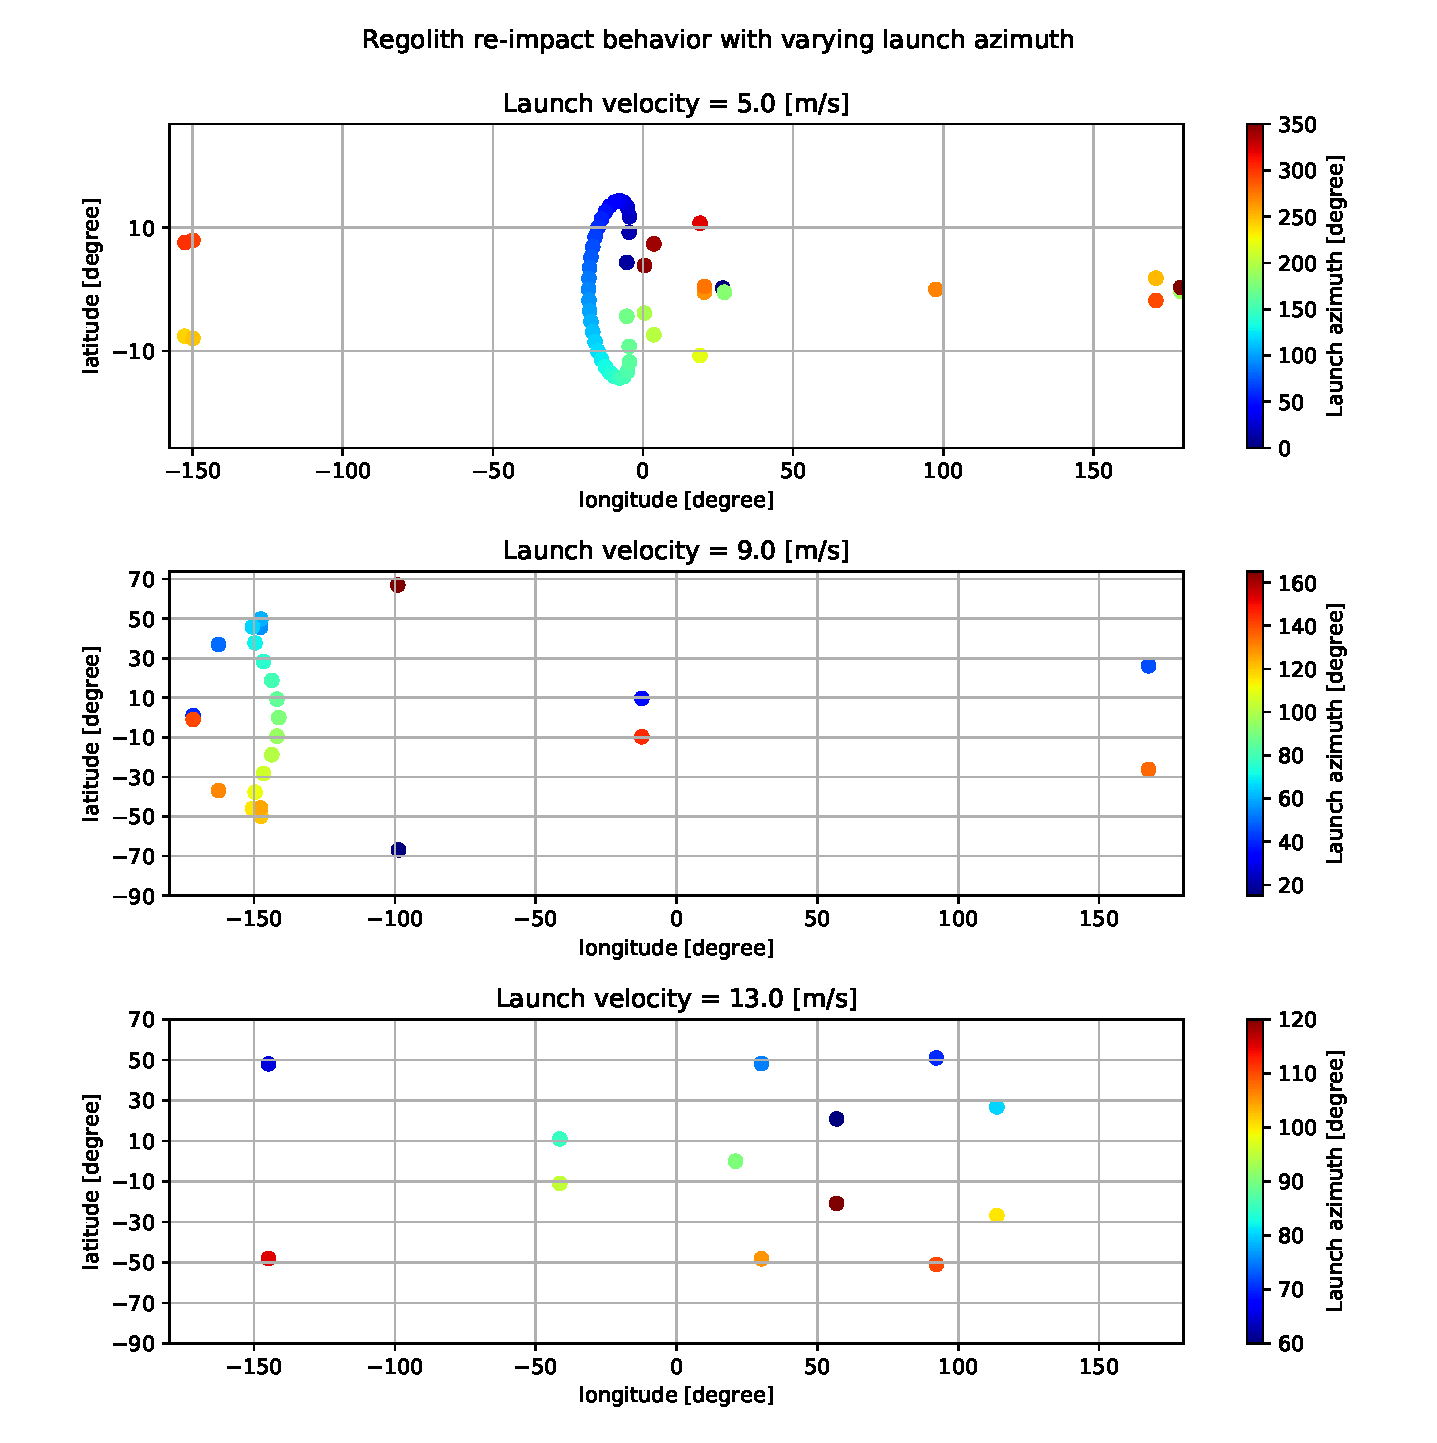
\includegraphics[angle=90, width=\textwidth, height=0.5\textheight, keepaspectratio=true]{longest_edge_perturbations/3.2Density_1cmSize/compare_with_noSP/three_velocity_crash_map_noSP.pdf}
    \label{fig:three_velocity_crashmap_comparison_noSP}
}

\subfloat[]{
    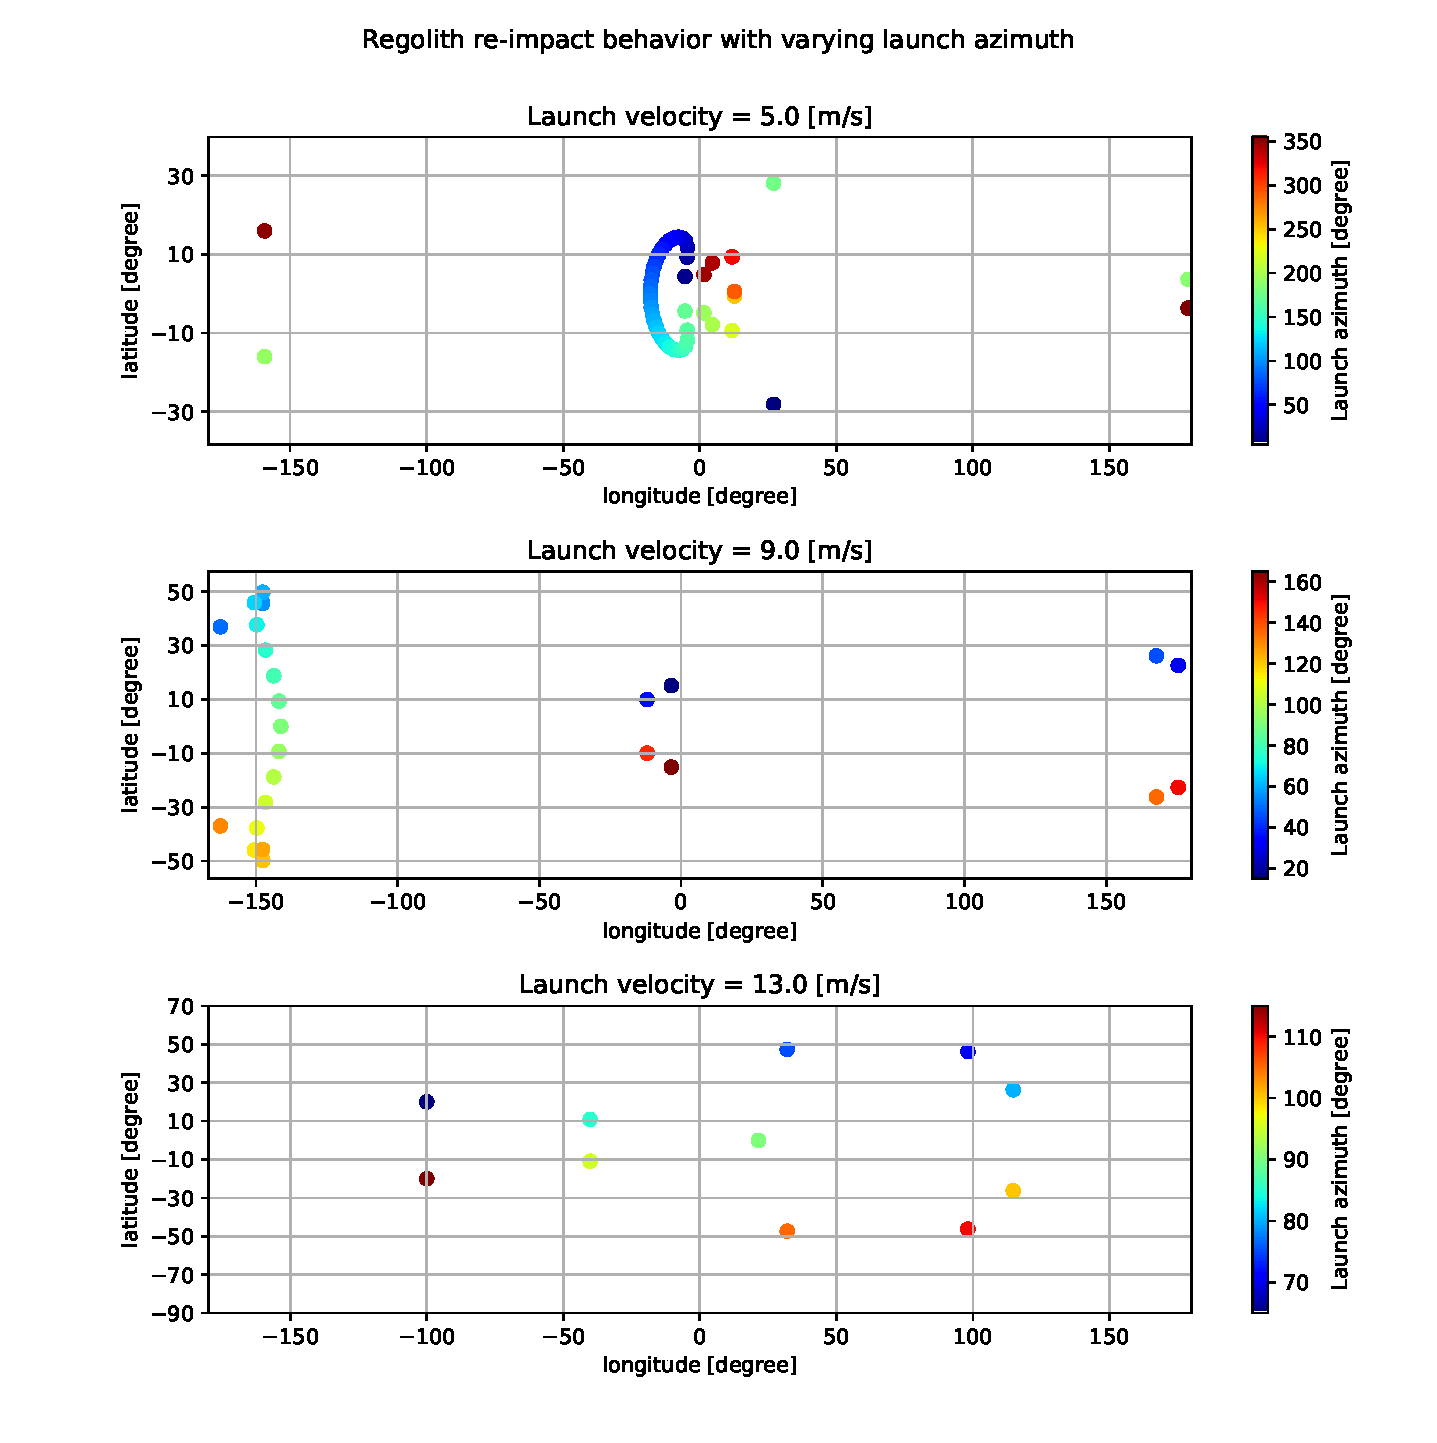
\includegraphics[angle=90, width=\textwidth, height=0.5\textheight, keepaspectratio=true]{longest_edge_perturbations/3.2Density_1cmSize/compare_with_noSP/three_velocity_crash_map_phase45.pdf}
    \label{fig:three_velocity_crashmap_comparison_sp}
}
\caption{Re-impact locations for three specific velocities, where for each velocity, the launch azimuth varies with a resolution of \SI{5}{\degree}. Out of the two figures, \protect\subref{fig:three_velocity_crashmap_comparison_noSP} shows the results for the unperturbed scenario and \protect\subref{fig:three_velocity_crashmap_comparison_sp} shows the results for the case with the perturbations. For the latter, the initial Solar phase angle is \SI{45}{\degree} and particle code is LoGSP-1.}
\label{fig:specific_velocity_crashMap_noSP_spanalysis}
\end{figure}
\FloatBarrier
%%%
%%%
\begin{figure}[htb]
\centering
\captionsetup{justification=centering}
\subfloat[]{
    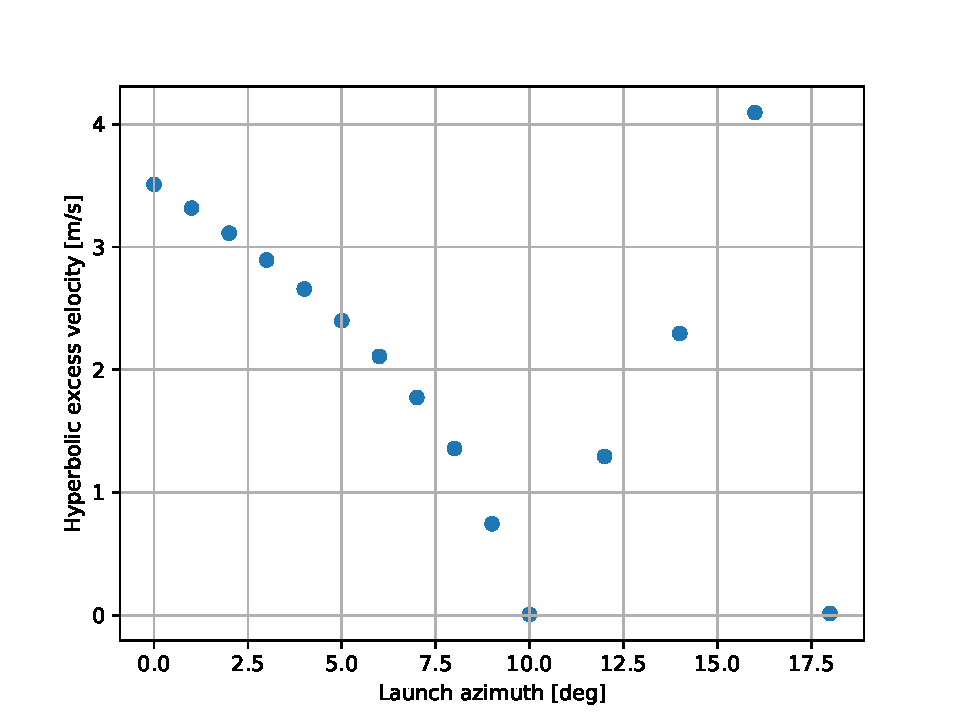
\includegraphics[angle=90, width=\textwidth, height=0.4\textheight, keepaspectratio=true]{longest_edge_perturbations/3.2Density_1cmSize/compare_with_noSP/escape_hev_9ms_phase45_1degAzimResolution.pdf}
    \label{fig:escape_hev_9ms_phase45}
}

\subfloat[]{
    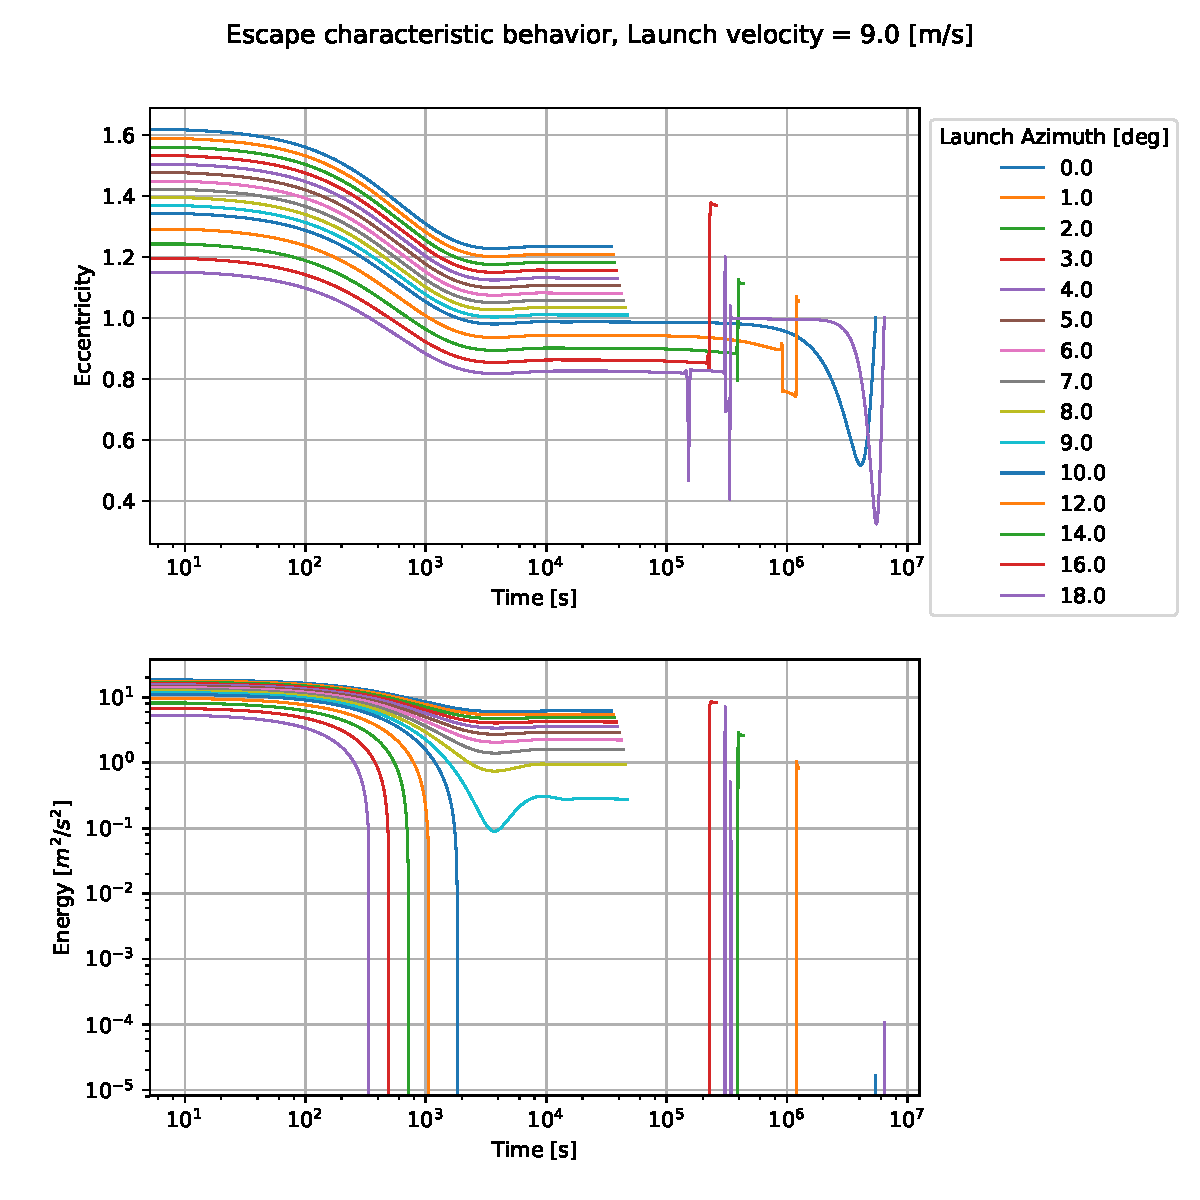
\includegraphics[angle=90, width=\textwidth, height=0.5\textheight, keepaspectratio=true]{longest_edge_perturbations/3.2Density_1cmSize/compare_with_noSP/escape_energy_ecc_9ms_phase45_1degAzimResolution.pdf}
    \label{fig:escape_energy_ecc_9ms_phase45}
}
\caption{Escape behavior for regolith launched with a velocity of \SI{9}{\metre\per\second}; launch azimuths shown here range from \SI{0}{\degree} to \SI{20}{\degree} in steps of \SI{1}{\degree}, which is sufficient to discuss the topic at hand. Out of the two figures, \protect\subref{fig:escape_hev_9ms_phase45} shows the \gls{HEV} data points and \protect\subref{fig:three_velocity_crashmap_comparison_sp} shows the energy and eccentricity curves for the corresponding cases. For the latter, the initial Solar phase angle is \SI{45}{\degree} and particle code is LoGSP-1.}
\label{fig:escape_9ms_noSP_spanalysis}
\end{figure}
\FloatBarrier
%%%

\subsection{Final Fate General Characteristics}
\label{subsec:final_fate_charac_general}
\Cref{fig:LoGSP_1_final_fate_histogram} gives a distribution of particles for each of the three different final fates for the regolith i.e. capture, re-impact, and escape, for different initial launch velocities and initial Solar phase angles. Irrespective of the initial Solar phase, initial launch velocities from 1.0 to \SI{3.0}{\metre\per\second} results in particles launched in all directions to eventually re-impact the asteroid's surface. Similarly, for initial launch velocities ranging from 14 to \SI{16.0}{\metre\per\second}, we see that the particles always manage to escape the gravitational attraction of the asteroid\footnote{There is one exception though, at \SI{14.0}{\metre\per\second} and for launch azimuth of \SI{90}{\degree} and Solar phase angle of \SI{315}{\degree}, the particle re-impacts}. Launch velocities from 4 to \SI{13.0}{\metre\per\second} show a mixed behavior and the final fate distribution trend does not vary drastically for different initial Solar phase angles. Looking at absolute numbers, for all Solar phase angles combined, about 54.9\% cases result in an escape situation, 44.8\% cases result in re-impact and a mere 0.2\% cases result in a capture scenario. Thus, the number of capture cases is extremely small relative to the other two final fates.
%
\newline\newline
%
For initial Solar phase of \SI{225.0}{\degree}, there are no cases of regolith being captured in orbit around the asteroid. All capture cases, arranged in order of increasing launch azimuth angle, are listed in \Cref{tab:LoGSP_1_capture}. It is interesting to note that all capture cases result from when the particle is launched in a direction which is against the direction of rotation of the asteroid.
%%%
\begin{table}[htb]
\centering
\captionsetup{justification=centering}
\caption{Initial conditions that resulted in temporary orbital capture of regolith around the asteroid. Particle code LoGSP-1.}
\label{tab:LoGSP_1_capture}
\begin{tabular}{|l|c|c|c|}
\hline
Index & \multicolumn{1}{l|}{Launch azimuth [deg]} & \multicolumn{1}{l|}{Launch velocity [m/s]} & \multicolumn{1}{l|}{Initial Solar phase angle [deg]} \\ \hline
\rowcolor[HTML]{FE996B}
1   & 5.0 & 5.0 & 315.0     \\ \hline
\rowcolor[HTML]{67FD9A}
2   & 10.0 & 9.0 & 135.0    \\ \hline
\rowcolor[HTML]{9698ED}
3   & 15.0 & 8.0 & 45.0     \\ \hline
\rowcolor[HTML]{FFCC67}
4   & 45.0 & 12.0 & 45.0    \\ \hline
\rowcolor[HTML]{96FFFB}
5   & 45.0 & 10.0 & 315.0   \\ \hline
\rowcolor[HTML]{FFCC67}
6   & 135.0 & 12.0 & 45.0   \\ \hline
\rowcolor[HTML]{96FFFB}
7   & 135.0 & 10.0 & 315.0  \\ \hline
\rowcolor[HTML]{9698ED}
8   & 165.0 & 8.0 & 45.0    \\ \hline
\rowcolor[HTML]{67FD9A}
9   & 170.0 & 9.0 & 135.0   \\ \hline
\rowcolor[HTML]{FE996B}
10  & 175.0 & 5.0 & 315.0   \\ \hline
% 11  & 185.0 & 5.0 & 135.0   \\ \hline
\end{tabular}
\end{table}
\FloatBarrier
%%%
The capture cases which represent symmetry in terms of the launch azimuth angle are highlighted with the same color in \Cref{tab:LoGSP_1_capture}. This symmetric behavior results from the combination of two factors. First, the Sun's motion relative to the asteroid is not in an inclined plane, and secondly, the particles are launched from the equatorial tip of the ellipsoid shaped asteroid, which is a point of symmetry on the ellipsoid. The capture cases are discussed in detail in \Cref{subsec:capture_orbit_analysis_as_is}.
%
\newline\newline
%
\Cref{fig:LoGSP_1_crashmap} depicts the surface distribution of regolith that re-impacts the surface when launched from the same location with different velocities and different initial Solar phase angles. The launch location is in the centre of the map, latitude and longitude \SI{0.0}{\degree}.
%%%
\begin{figure}[htb]
\centering
\captionsetup{justification=centering}
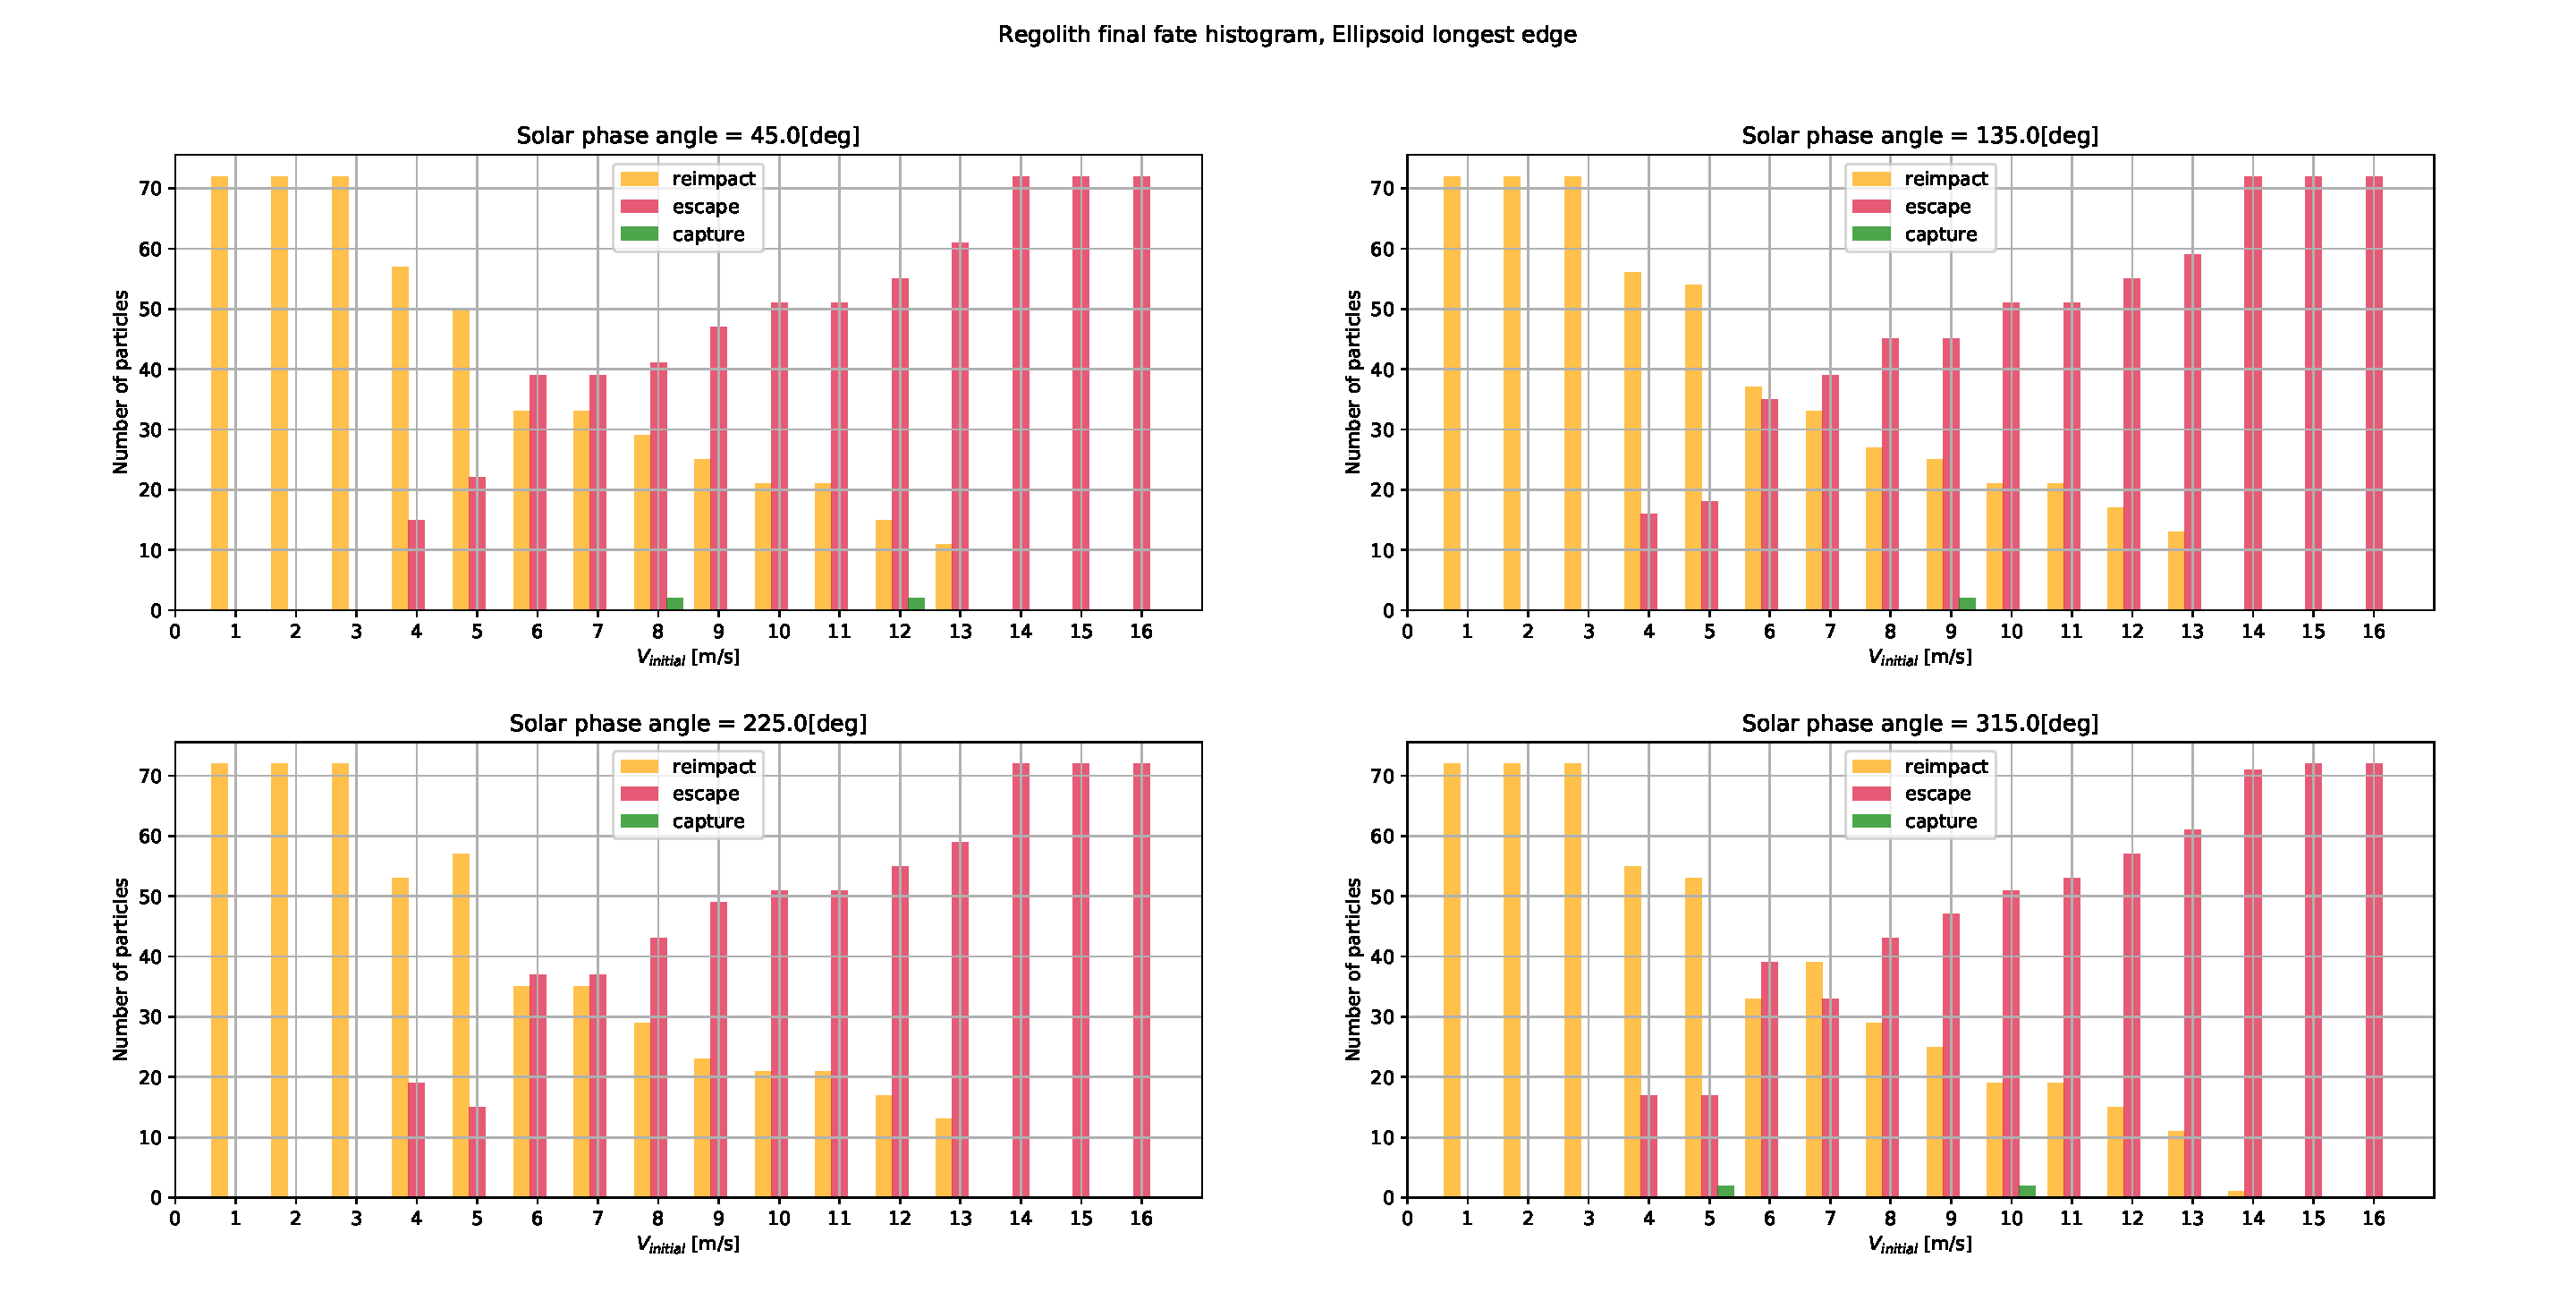
\includegraphics[angle=90, width=\textwidth, height=\textheight, keepaspectratio=true]{longest_edge_perturbations/3.2Density_1cmSize/final_fate_versus_launch_velocity_histogram_all_solar_phases.pdf}
\caption{Histogram showing the number of particles that re-impact, escape, or get captured around the asteroid, for different initial launch velocities. Particle code LoGSP-1.}
\label{fig:LoGSP_1_final_fate_histogram}
\end{figure}
\FloatBarrier
%%%
The re-impact locations remains unchanged, irrespective of the initial Solar phase angles, for all particles launched with the relatively lower velocities (1 to \SI{4}{\metre\per\second}). Again for the mid-range velocities, i.e. 5 to \SI{9}{\metre\per\second}, the re-impact locations for the particles that are launched in the direction opposite to the asteroid's rotation remains unchanged for different initial Solar phase angles. This can be observed in the arc shaped re-impact location patterns West of the launch location for those velocities. The distribution pattern, for all launch velocities and initial Solar phases, is also symmetric about the equator. Again, the reason for this is the same as mentioned earlier for the symmetry in capture cases in \Cref{tab:LoGSP_1_capture}. In general, keeping the launch direction and velocity constant, we see that the distribution of re-impact locations does not change drastically with varying initial Solar phase angles. This is much easily observed in a plot of the range from the launch site to the re-impact point versus launch azimuth for different velocities as shown in \Cref{fig:LoGSP_1_range_comparison}.
% %
% \newline\newline
% %
% We have not shown the range to re-impact point plots in \Cref{fig:LoGSP_1_range_comparison} for all launch velocities because the intention here is to show the qualitative behavior, which can be achieved by considering only a subset of the launch velocities that result in a re-impact scenario. The very first thing we observe is that as the launch velocity increases, the range of launch azimuth over which the regolith re-impacts the surface reduces because a higher velocity allows the regolith to enter a higher orbit (as it attains a relatively higher energy) and reduces the probability of a re-impact. Even as the velocity increases, we see that the azimuths that result in a re-impact are the ones in which the regolith is launched in a direction that is opposite to the asteroid's rotation direction. This makes sense since the regolith's energy would be reduced the most in this scenario compared to all other launch directions, thereby increasing the chances of a re-impact.
% %
% \newline\newline
% %
% Now the primary purpose of the plots in \Cref{fig:LoGSP_1_range_comparison} (combined with \Cref{fig:LoGSP_1_crashmap}) is to depict the qualitative effect of Solar perturbations, for varying initial Solar phase angles, on the re-impact behavior of regolith compared to the case when no Solar perturbations are considered. For launch velocities of 4.0, 7.0 and \SI{10.0}{\metre\per\second}, we see that the Solar perturbations do not affect the re-impact location for cases when the particle is launched in directions opposite to that of the asteroid's rotation. However, we do see few exceptions to the former statement, most noticeably in the case of \SI{7.0}{\metre\per\second}. But for the majority of cases where the re-impact location remains unchanged, we see from \Cref{fig:LoGSP_1_reimpact_time}, that these particles spend less than 3.0 hours in orbit which is not enough time for the Solar perturbations to act and have any significant impact on the dynamics of the particles. So in essence this is what is happening here - particles when launched in a direction that is opposite to that of the asteroid's rotation, even at relatively high velocities such as \SI{10.0}{\metre\per\second}, loose enough energy to stay in a relatively lower orbit (see \Cref{fig:LoGSP_1_maxAltitude_reimpactscenario}) where the gravitational force of the asteroid is significantly stronger than any of the Solar perturbations and as the particle spends a very short time in orbit before re-impact, the Solar perturbations do not get enough time to affect the particle's orbit and hence the particle re-impacts the same location as it would have when no Solar perturbations were considered in the simulation. For the lower launch velocities of 4.0 and \SI{7.0}{\metre\per\second}, the differences in re-impact locations are more pronounced when the regolith is launched in the same direction as that of the asteroid's rotation. Particles gain relatively higher energy in this case, enter a higher orbit and spend enough time there for the Solar perturbations to affect its motion. For the case of the launch velocity of \SI{13.0}{\metre\per\second} in \Cref{fig:LoGSP_1_range_comparison}, the velocity is high enough such that the particle does not loose enough energy when launched opposite to the asteroid's rotational direction and is able to enter a relatively higher orbit (see \Cref{fig:LoGSP_1_maxAltitude_reimpactscenario}) and stay there for a relatively longer time, as seen in \Cref{fig:LoGSP_1_reimpact_time}, which results in the Solar perturbations affecting the orbital motion and eventually the re-impact location of the regolith.
%%%
\begin{figure}[htb]
\centering
\captionsetup{justification=centering}
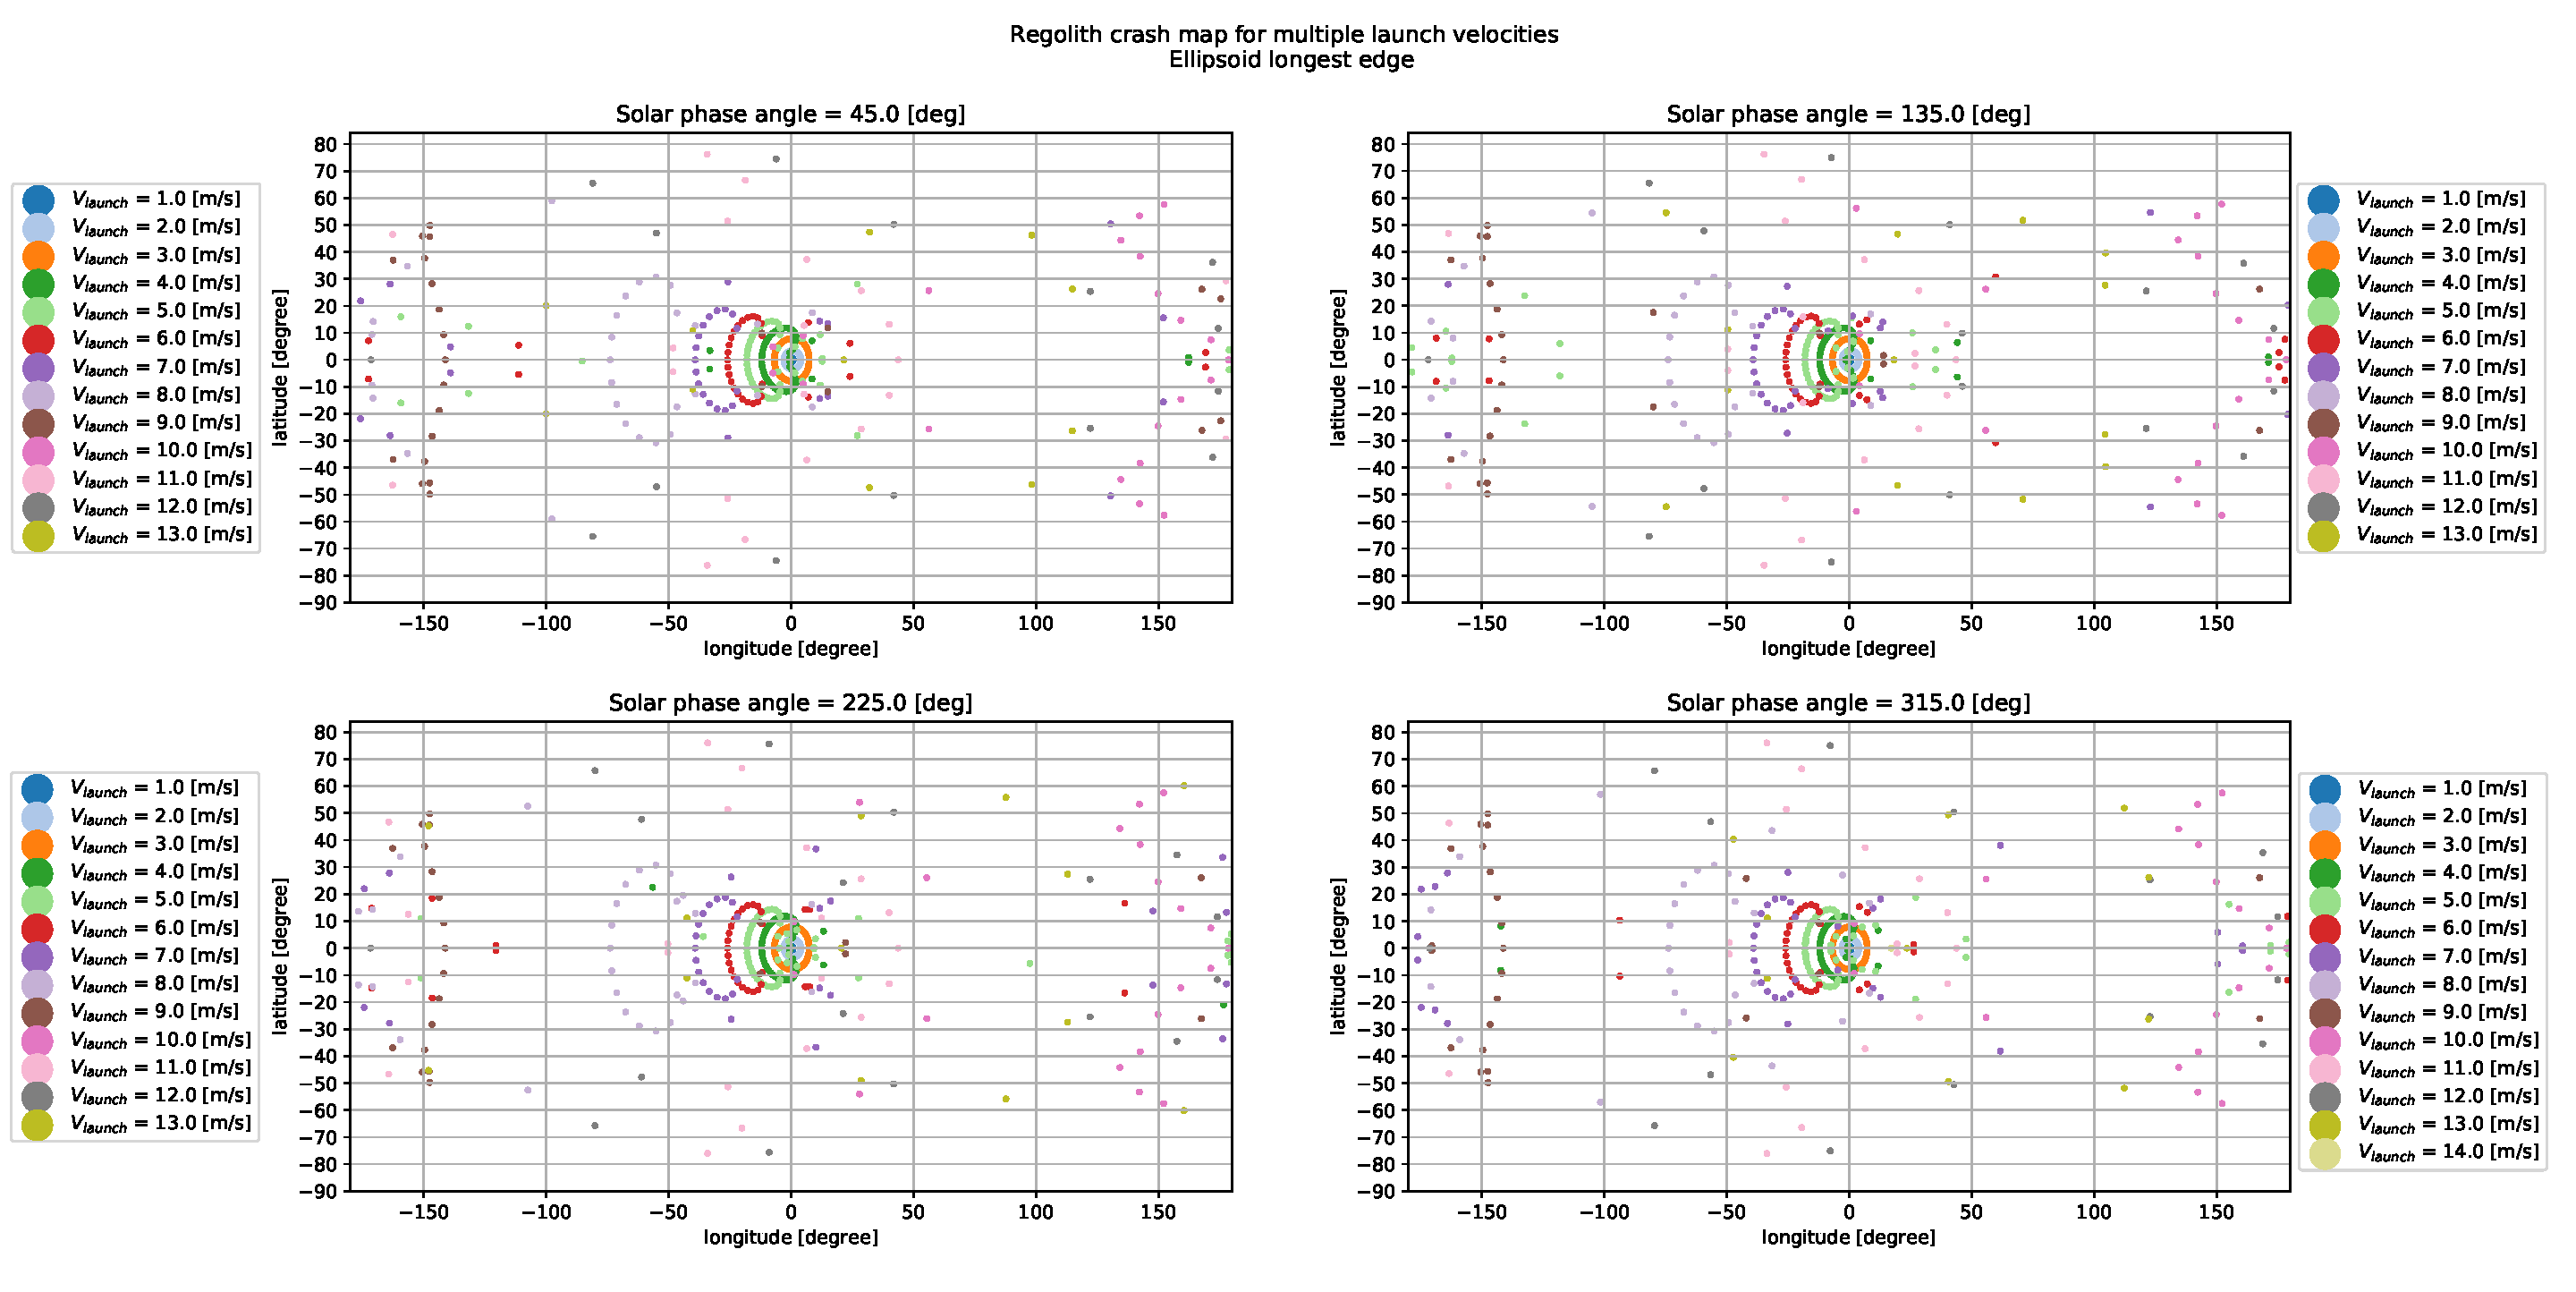
\includegraphics[angle=90, width=\textwidth, height=\textheight, keepaspectratio=true]{longest_edge_perturbations/3.2Density_1cmSize/crash_map_all_solar_phases.pdf}
\caption{Surface distribution of re-impacted regolith for different launch velocities. The launch location is \\ latitude: \SI{0}{\degree}, longitude: \SI{0.0}{\degree}. Particle code LoGSP-1.}
\label{fig:LoGSP_1_crashmap}
\end{figure}
\FloatBarrier
%%%

\subsection{Capture Orbit Analysis}
\label{subsec:capture_orbit_analysis_as_is}
We shall now look at the cases where the lofted regolith gets (temporarily) captured in orbit by the asteroid. The initial conditions for all capture cases, for the current particle size and density, were mentioned earlier in \Cref{tab:LoGSP_1_capture}. \Cref{fig:LoGSP_1_capture_orbital_range} depicts the progression in orbital range of the temporarily captured regolith. The straight lines in the plot are used to mark the different altitude regimes. These are the \gls{LAO}, \gls{MAO}, \gls{HAO}, \gls{UHAO}, and \gls{EHAO}. These altitude regime definitions are not from well defined standards, but instead were arbitrarily chosen as integer multiples of the longest semi-axis, $\alpha$, of the tri-axial ellipsoid shaped asteroid. The definition for these altitude regimes is given in \Cref{tab:altitude_regimes}.
%%%
\begin{table}[htb]
\centering
\captionsetup{justification=centering}
\caption{Altitude regimes and their definitions}
\label{tab:altitude_regimes}
\begin{tabular}{|c|c|}
\hline
\textbf{Altitude regime}        & \textbf{Definition}                    \\ \hline
\gls{LAO}                       & Asteroid surface to $2 \times \alpha$  \\ \hline
\gls{MAO}                       & $2 \times \alpha$ to $3 \times \alpha$ \\ \hline
\gls{HAO}                       & $3 \times \alpha$ to $5 \times \alpha$ \\ \hline
\gls{UHAO}                      & $5 \times \alpha$ to $7 \times \alpha$ \\ \hline
\gls{EHAO}                      & Above $7 \times \alpha$                \\ \hline
\end{tabular}
\end{table}
\FloatBarrier
%%%
The purpose of plotting data as shown in \Cref{fig:LoGSP_1_capture_orbital_range} was to look for any patterns or periodicity, if they existed, and to see if particles in temporary capture scenario remain closer to the asteroid or further away from it. The symmetry as explained for initial conditions mentioned in \Cref{tab:LoGSP_1_capture} can also be seen in \Cref{fig:LoGSP_1_capture_orbital_range}, for example, regolith launched with velocity of \SI{8.0}{\metre\per\second} and launch azimuth of \SI{15.0}{\degree} (shown by the purple curve in the top plot in \Cref{fig:LoGSP_1_capture_orbital_range}) shows the same behavior as that of regolith launched with the same velocity and \SI{165.0}{\degree} launch azimuth (shown by the green curve in the bottom plot in \Cref{fig:LoGSP_1_capture_orbital_range}). Another thing we see from the plot is that the captured regolith stay in the higher altitude regions for most part and only briefly do they fall within the \gls{MAO} and \gls{LAO} region. We shall now take a look at a few cases from \Cref{fig:LoGSP_1_capture_orbital_range} in a bit more detail to understand the effect of Solar perturbations by comparing these cases with their unperturbed counterparts.
%
\newline\newline
%
Of all the cases shown in \Cref{fig:LoGSP_1_capture_orbital_range} or \Cref{tab:LoGSP_1_capture}, the one with a launch velocity of \SI{10.0}{\metre\per\second} and launch azimuth of \SI{45.0}{\degree} results in a re-impact scenario when Solar perturbations are omitted, but the same initial conditions lead to a temporary capture orbit when perturbations were added for an initial Solar phase angle of \SI{315.0}{\degree}. Every other initial condition for the capture cases had otherwise resulted in an escape situation when simulations were conducted without the Solar perturbations. The 3D trajectory plot in two different views for the former case are shown in \Cref{fig:LoGSP_1_capture_case_5_3d_traj_inertialFrame_differnetViews} (see \Cref{fig:LoGSP_1_capture_case_5_3d_trajectory} also for the 3D trajectory representation in the \gls{ARF}). The 2D trajectory for the same is shown in \Cref{fig:LoGSP_1_capture_case_5_2d_traj_inertialFrame} in inertial frame and in \Cref{fig:LoGSP_1_capture_case_5_2d_traj_bodyFrame} in the \gls{ARF} or the body frame. The web-link or URL for the trajectory animation of the particle (in inertial frame and in XY-plane only) can be found in \Cref{fig:LoGSP_1_capture_case_5_2d_trajectory_animation}.
%%%
\begin{figure}[htb]
\centering
\captionsetup{justification=centering}

\includegraphics[scale=0.2]{longest_edge_perturbations/3.2Density_1cmSize/qrcode_10ms_45Azimuth_315SolarPhase.png}
\caption{2D trajectory animation (XY-Plane) of capture regolith for case number 5 in \Cref{tab:LoGSP_1_capture}. Particle code LoGSP-1. Scan the QR code to view the animation or use the following web-link: \url{https://youtu.be/oZDhDo5CIsk}}
\label{fig:LoGSP_1_capture_case_5_2d_trajectory_animation}
\end{figure}
\FloatBarrier
%%%
%%%
\begin{figure}[htb]
\centering
\captionsetup{justification=centering}
% another option for includegraphics - keepaspectratio
\subfloat[]{
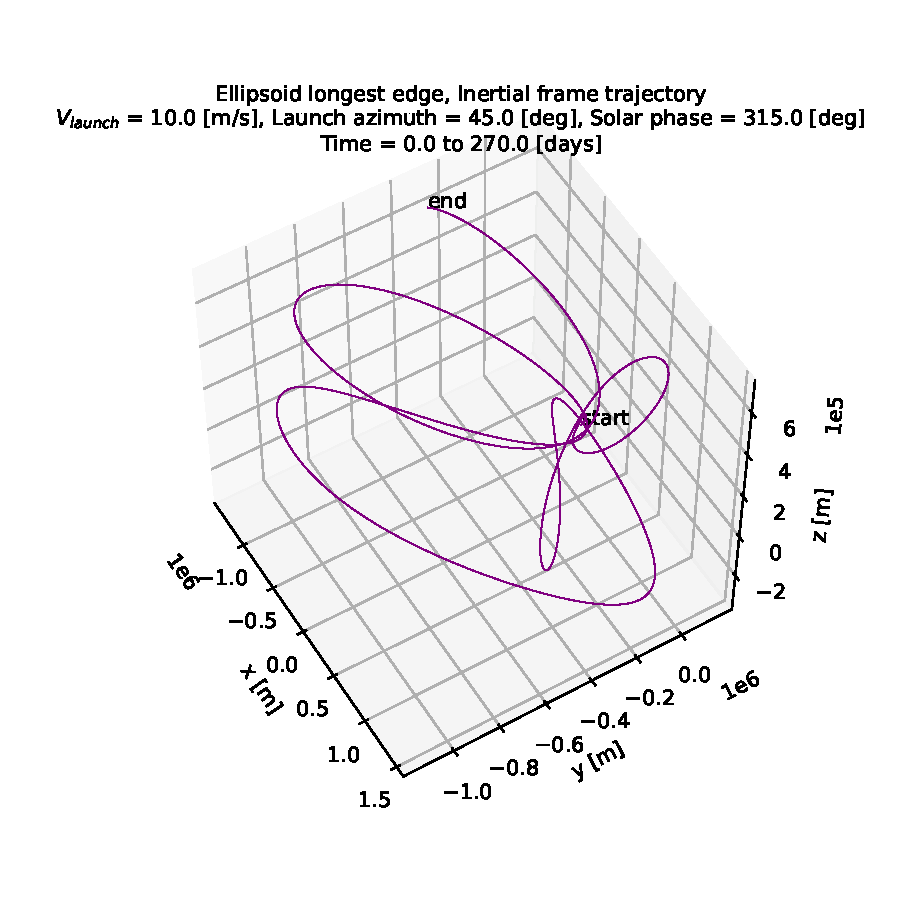
\includegraphics[width=0.5\textwidth, height=0.5\textheight, keepaspectratio=true]{longest_edge_perturbations/3.2Density_1cmSize/3dTrajectory_10ms_45Azimuth_315solarPhase_inertialFrame_View1.pdf}
}
\subfloat[]{
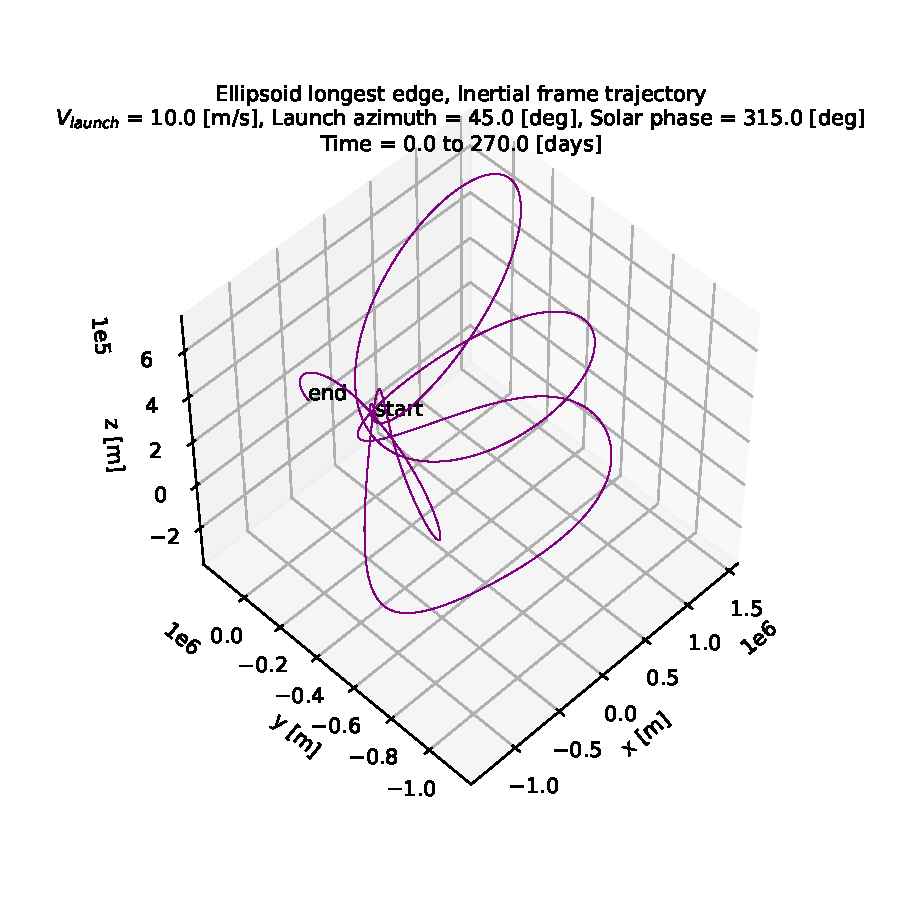
\includegraphics[width=0.5\textwidth, height=0.5\textheight, keepaspectratio=true]{longest_edge_perturbations/3.2Density_1cmSize/3dTrajectory_10ms_45Azimuth_315solarPhase_inertialFrame_View2.pdf}
}
\caption{3D inertial frame trajectory of capture regolith for case number 5 in \Cref{tab:LoGSP_1_capture} in two different viewing angles. Particle code LoGSP-1.}
\label{fig:LoGSP_1_capture_case_5_3d_traj_inertialFrame_differnetViews}
\end{figure}
\FloatBarrier
%%%
Note that in the trajectory animation in \Cref{fig:LoGSP_1_capture_case_5_2d_trajectory_animation} (and any other animation included henceforth) the particle is made to skip several data points in between along the trajectory when it is far away from the asteroid, just to reduce the length of the animation. So because of this, the particle appears to be moving faster when it is away from the asteroid but this is not true. For the exact velocity of the particle, the reader should look at the velocity magnitude indicator within the animation itself.
%
\newline\newline
%
The animation shows that the particle reverses its direction of motion twice in its entire course. To visualize how this is happening in 3D, look at \Cref{fig:LoGSP_1_capture_case_5_3d_traj_inertialFrame_differnetViews}. The reason for this can be understood by looking at the direction of the perturbing acceleration, the gravitational acceleration vectors, and the combined effect of all accelerations acting on the particle. The direction of \gls{SRP} and \gls{STBE} are shown in \Cref{fig:LoGSP_1_capture_case_5_2d_trajectory_srp_stbe_perturbationVectors} and that of the net effect of the two is shown in \Cref{fig:LoGSP_1_capture_case_5_2d_trajectory_totalPerturbationVectors}. In the trajectory simulator, the gravity model (triaxial ellipsoid model) computes the acceleration in the rotating frame. We calculated the direction of the gravitational acceleration in the \gls{AIF} in post-simulation analysis assuming a point-mass model by considering the fact that when the regolith is far away from the asteroid, its gravity field would appear as that of a point-mass gravity source. The gravitational acceleration vectors are shown in \Cref{fig:LoGSP_1_capture_case_5_2d_trajectory_gravityVector}. The net acceleration acting on the particle is then shown in \Cref{fig:LoGSP_1_capture_case_5_2d_totalAccelerationVector_inertialFrame}. All acceleration vectors are shown along those parts of the trajectory where the magnitude of \gls{SRP} acceleration is of the same order of magnitude as that of the gravitational acceleration. However, the magnitude of the \gls{STBE} acceleration is always one order of magnitude smaller than the gravitational acceleration for those very same points along the trajectory, but is still significant. We do not show the vectors for the entire trajectory for two reasons; first, when close to the asteroid the direction of these vectors would reduce the clarity of the plot and,  second, we want to discuss the effect of the perturbations when the particle is far away from the asteroid because then they are as significant as the gravitational force.
%
\newline\newline
%
In \Cref{fig:LoGSP_1_capture_case_5_2d_traj_inertialFrame}, the trajectory loops numbered 1 and 2 (XY-plane), is where the particle's direction of motion gets reversed. If we look at \Cref{fig:LoGSP_1_capture_case_5_2d_trajectory_srpVectors}, we see that the direction of the \gls{SRP} vector is consistent with how the particle changes its direction of motion. This, however, does not mean that the \gls{SRP} is the sole actor responsible for how the particle's motion eventually turns out to be (and we will see this in detail shortly). The direction of \gls{STBE}, as shown in \Cref{fig:LoGSP_1_capture_case_5_2d_trajectory_stbeVectors}, however, does not directly tell us on how the particle's motion would change as it progresses through its trajectory. \gls{STBE} is always an order of magnitude smaller than \gls{SRP} for the points shown in the two plots and its direction is not consistent with how the particle changes its direction of motion, but its contribution to the capture scenario is significant (we will see the effect of removing \gls{STBE} shortly). The direction of the net perturbing acceleration, shown in \Cref{fig:LoGSP_1_capture_case_5_2d_trajectory_totalPerturbationVectors}, shows us exactly how and where the motion of the particle is directed. Especially when we look at trajectory loops 1 and 2 in \Cref{fig:LoGSP_1_capture_case_5_2d_traj_inertialFrame}, we can see that the net perturbing vector is acting in the direction that is consistent with how the particle changes its orbital motion. Now looking at these plots that we just discussed, a question that arises is why did the particle remain in a temporary capture orbit, and for example not escape especially when the net perturbing acceleration was acting opposite to the direction of asteroid such as in trajectory loop number 3 in \Cref{fig:LoGSP_1_capture_case_5_2d_traj_inertialFrame}? The answer to this is found by looking at the direction of gravitational attraction in \Cref{fig:LoGSP_1_capture_case_5_2d_trajectory_gravityVector} and the total acceleration (i.e. the net effect of gravity and perturbations) acting on the particle in \Cref{fig:LoGSP_1_capture_case_5_2d_totalAccelerationVector_inertialFrame}. Although the gravitational acceleration has the same order of magnitude as that of the Solar perturbations when the particle is far away from the asteroid, we see that the net effect of the two is towards the asteroid and hence prevents the particle from escaping.
%%%
\begin{figure}[htb]
\centering
\captionsetup{justification=centering}
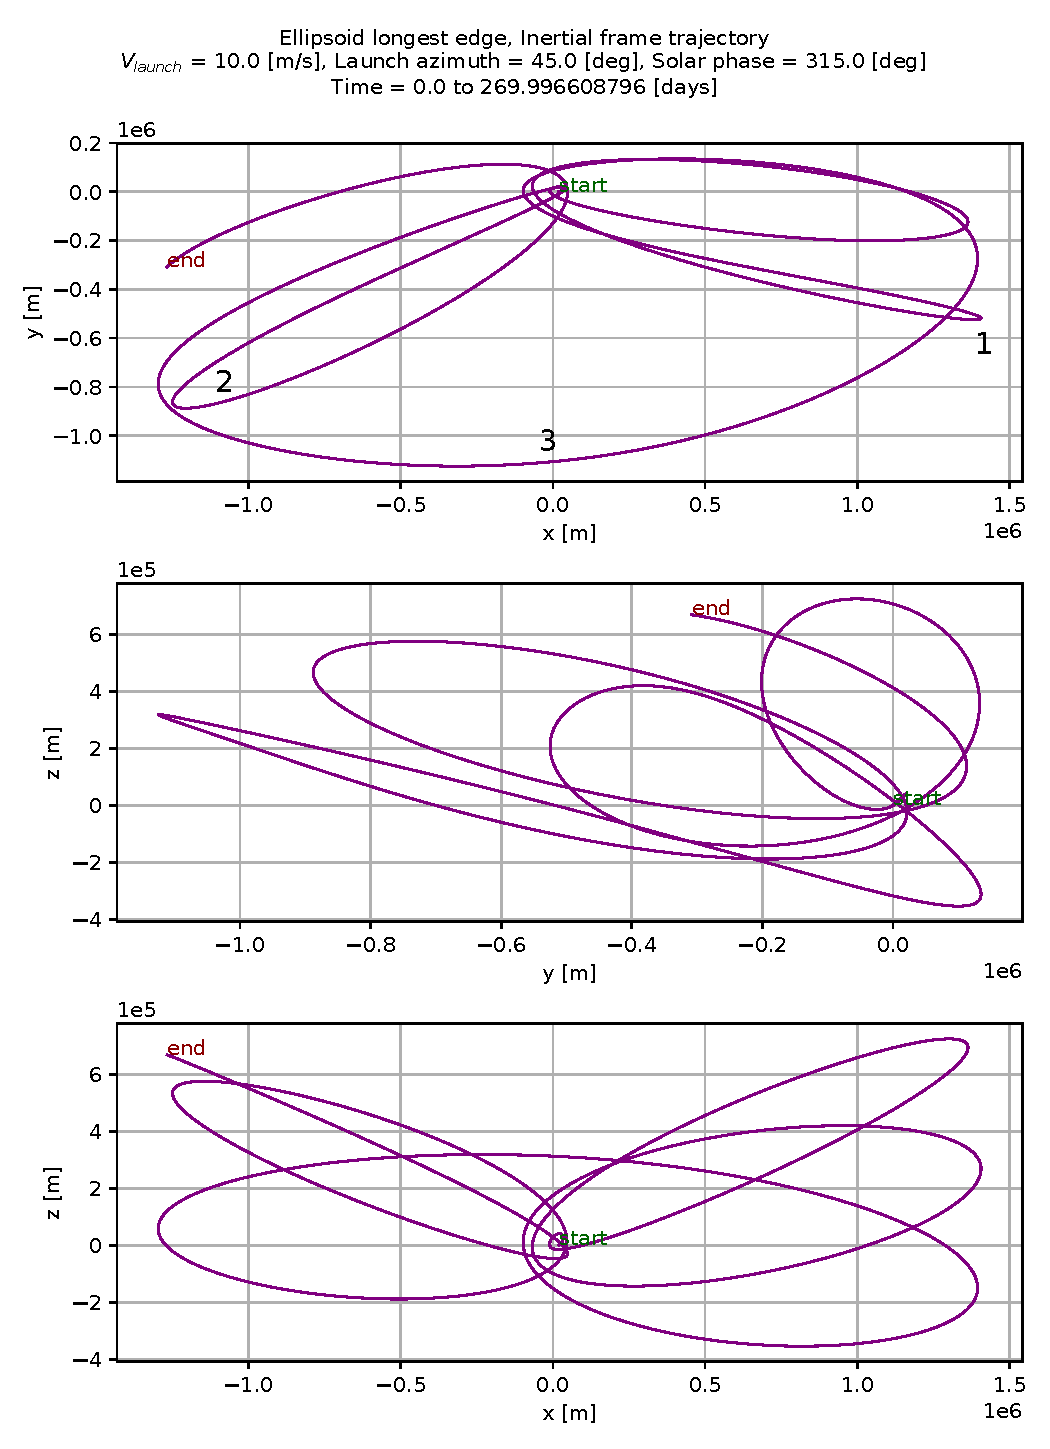
\includegraphics[angle=90, width=\linewidth, height=\textheight, keepaspectratio=true]{longest_edge_perturbations/3.2Density_1cmSize/10ms_45Azimuth_315SolarPhase/2d_trajectory_inertialFrame_edit.pdf}
\caption{2D inertial frame trajectory of capture regolith for case number 5 in \Cref{tab:LoGSP_1_capture}. Particle code LoGSP-1.}
\label{fig:LoGSP_1_capture_case_5_2d_traj_inertialFrame}
\end{figure}
\FloatBarrier
%%%
%%%
\begin{figure}[htb]
\centering
\captionsetup{justification=centering}
\subfloat[]
{
    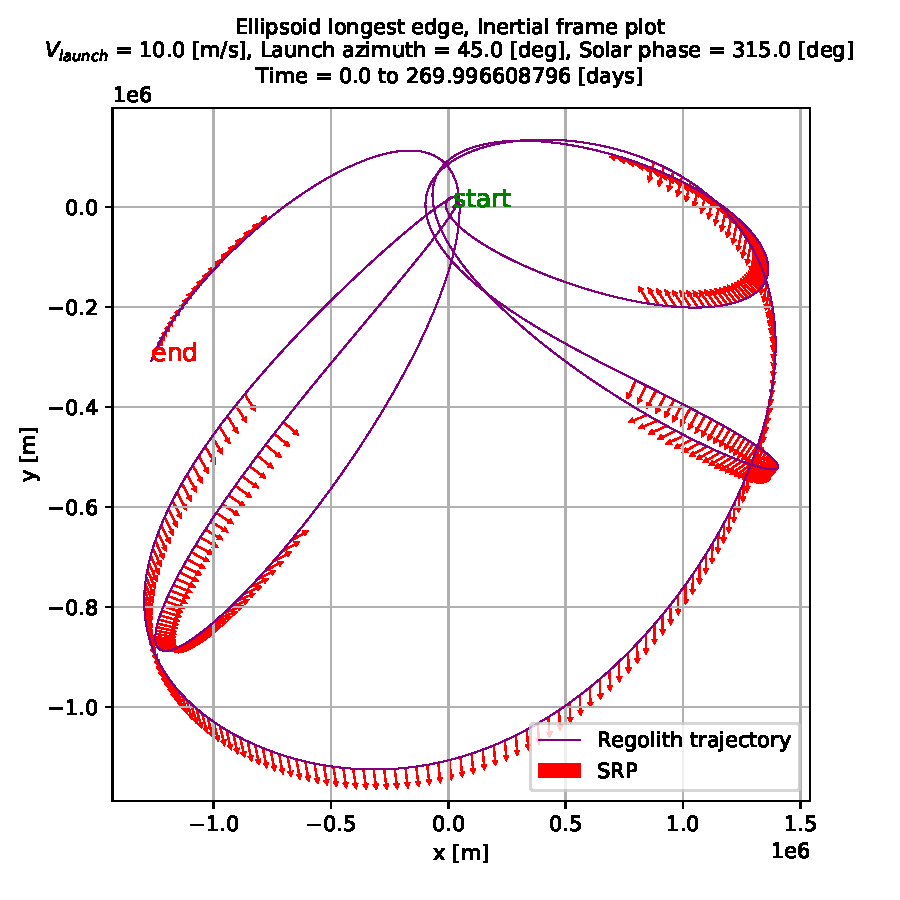
\includegraphics[width=0.5\linewidth, height=0.45\textheight, keepaspectratio=true]{longest_edge_perturbations/3.2Density_1cmSize/10ms_45Azimuth_315SolarPhase/srp_inertialFrame.pdf}
    \label{fig:LoGSP_1_capture_case_5_2d_trajectory_srpVectors}
}
\subfloat[]
{
    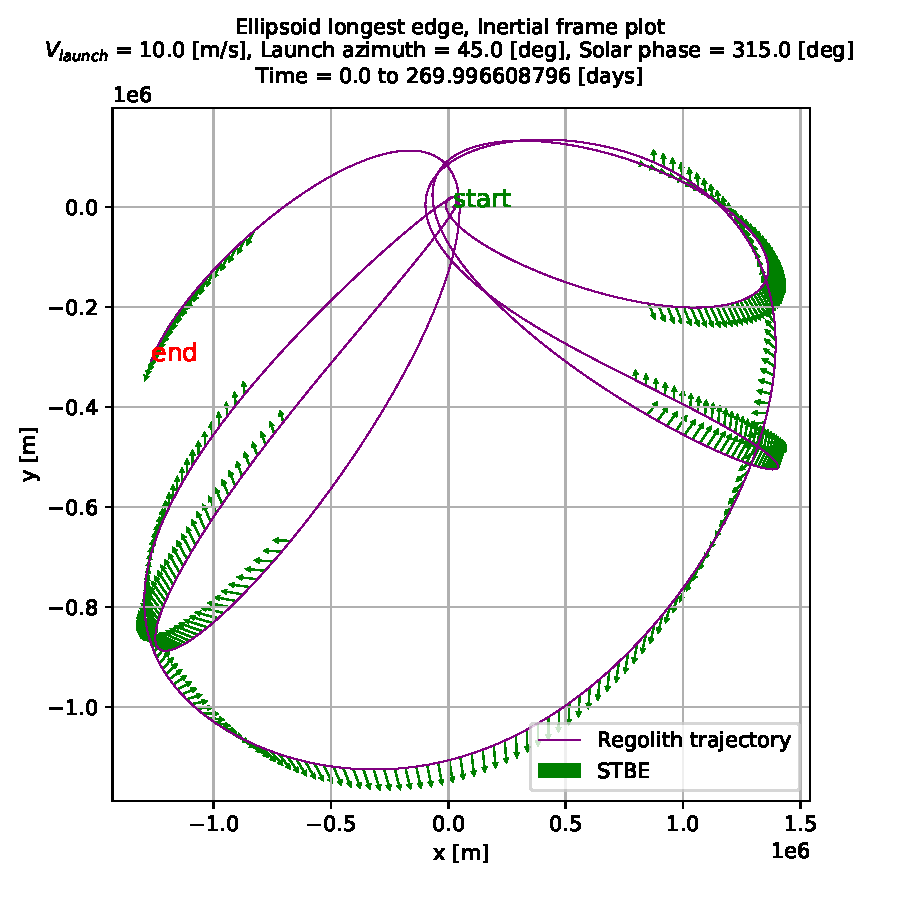
\includegraphics[width=0.5\linewidth, height=0.45\textheight, keepaspectratio=true]{longest_edge_perturbations/3.2Density_1cmSize/10ms_45Azimuth_315SolarPhase/stbe_inertialFrame.pdf}
    \label{fig:LoGSP_1_capture_case_5_2d_trajectory_stbeVectors}
}
\caption{2D trajectory of capture regolith for case number 5 in \Cref{tab:LoGSP_1_capture} with direction of \gls{SRP} and \gls{STBE} perturbation vectors. Note that the vectors are shown only for those parts of the trajectory where the \gls{SRP} magnitude is of the same order as that of the asteroid's gravitational acceleration. For those very same points along the trajectory, the magnitude of the \gls{STBE} is always one order of magnitude smaller than the gravitational acceleration. Particle code LoGSP-1.}
\label{fig:LoGSP_1_capture_case_5_2d_trajectory_srp_stbe_perturbationVectors}
\end{figure}
\FloatBarrier
%%%
%%%
\begin{figure}[htb]
\centering
\captionsetup{justification=centering}
\subfloat[]{
    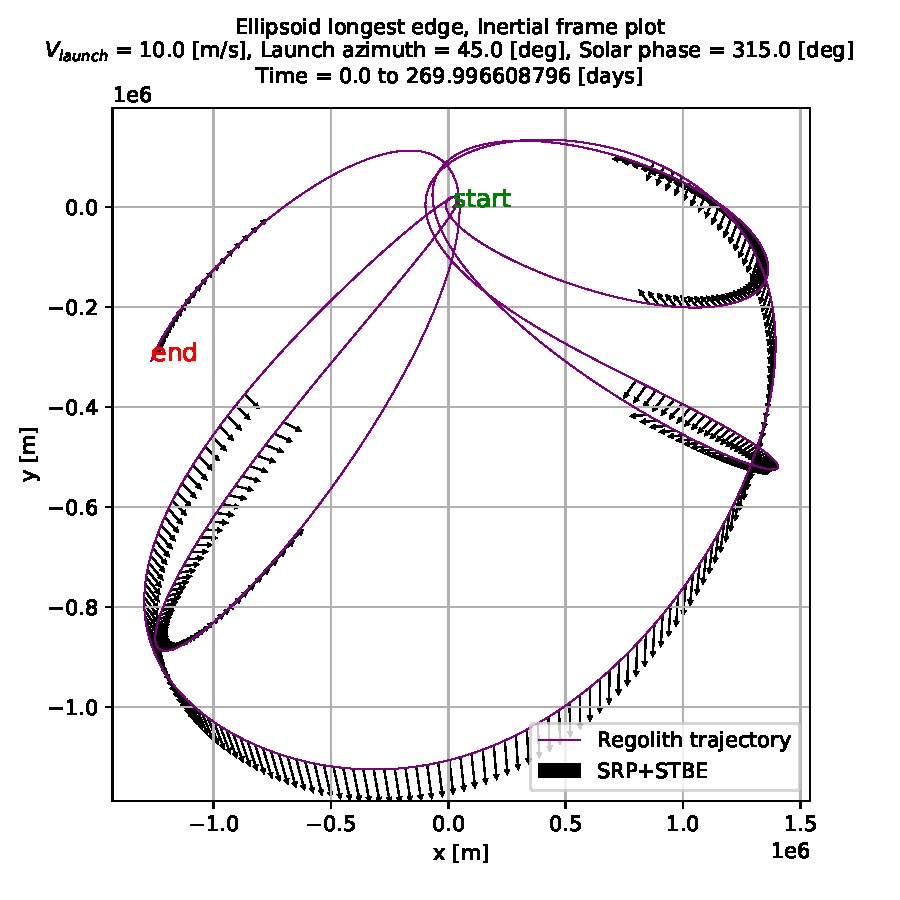
\includegraphics[width=0.5\linewidth, height=0.45\textheight, keepaspectratio=true]{longest_edge_perturbations/3.2Density_1cmSize/10ms_45Azimuth_315SolarPhase/totalPerturbation_inertialFrame.pdf}
    \label{fig:LoGSP_1_capture_case_5_2d_trajectory_totalPerturbationVectors}
}
\subfloat[]
{
    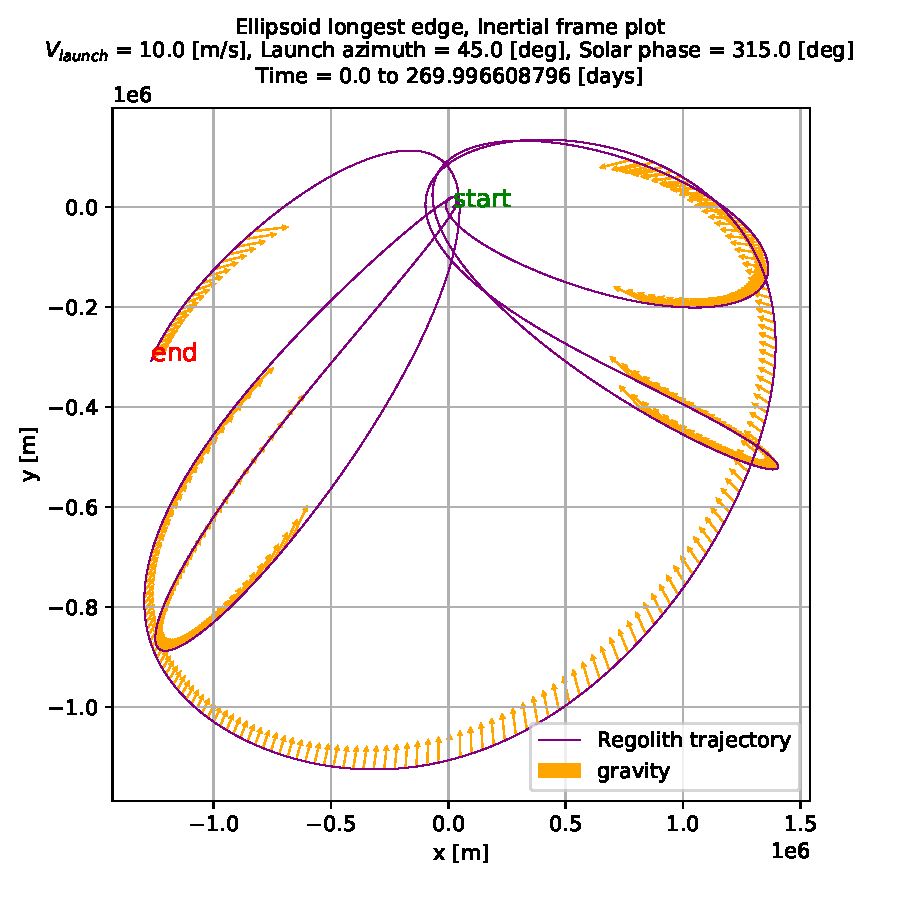
\includegraphics[width=0.5\linewidth, height=0.45\textheight, keepaspectratio=true]{longest_edge_perturbations/3.2Density_1cmSize/10ms_45Azimuth_315SolarPhase/gravity_inertialFrame.pdf}
    \label{fig:LoGSP_1_capture_case_5_2d_trajectory_gravityVector}
}
\caption{2D trajectory of capture regolith for case number 5 in \Cref{tab:LoGSP_1_capture} with direction of the sum total of \gls{SRP} and \gls{STBE} perturbation vectors, and the direction of the gravitational acceleration vector for the same data points. Note that the vectors are shown only for those parts of the trajectory where the \gls{SRP} magnitude is of the same order as that of the asteroid's gravitational acceleration. For those very same points along the trajectory, the magnitude of the \gls{STBE} is always one order of magnitude smaller than the gravitational acceleration. Particle code LoGSP-1.}
\end{figure}
\FloatBarrier
%%%
%%%
\begin{figure}[htb]
\centering
\captionsetup{justification=centering}
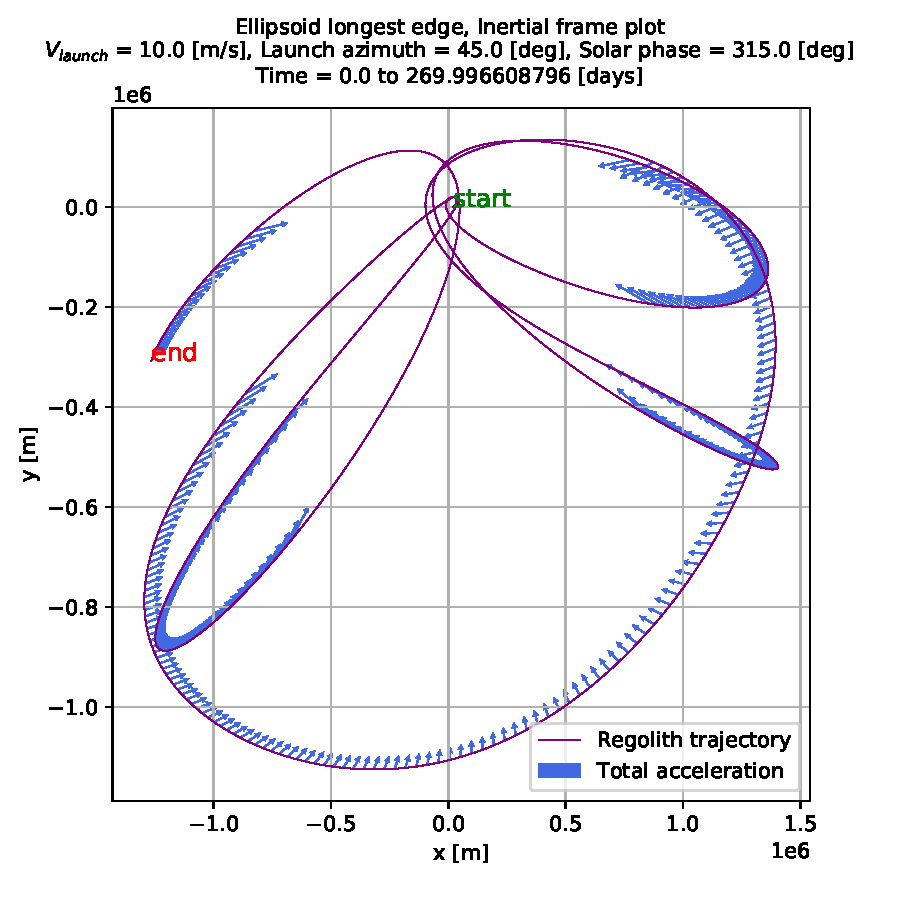
\includegraphics[width=\linewidth, height=0.4\textheight, keepaspectratio=true]{longest_edge_perturbations/3.2Density_1cmSize/10ms_45Azimuth_315SolarPhase/totalAcceleration.pdf}
\caption{2D trajectory of capture regolith for case number 5 in \Cref{tab:LoGSP_1_capture} with direction of the net acceleration vector. Note that the vectors are shown only for those parts of the trajectory where the \gls{SRP} magnitude is of the same order as that of the asteroid's gravitational acceleration. For those very same points along the trajectory, the magnitude of the \gls{STBE} is always one order of magnitude smaller than the gravitational acceleration. Particle code LoGSP-1.}
\label{fig:LoGSP_1_capture_case_5_2d_totalAccelerationVector_inertialFrame}
\end{figure}
\FloatBarrier
%%%
Both \gls{SRP} and \gls{STBE} together are necessary in getting the capture trajectory shown in \Cref{fig:LoGSP_1_capture_case_5_2d_traj_inertialFrame}. If either one of them is removed from the simulation, for the same launch conditions and initial Solar phase angle, then the results are completely different and we do not get a capture orbit. Note that the definition of capture orbit in this context implies that the particle stays in an orbit around the asteroid for the complete duration of 270 days, i.e., the maximum time for which the simulation is run.

\subsubsection{Effects of omitting Solar Third Body Effect (STBE)}
When only \gls{STBE} is removed, we get a trajectory where the particle eventually escapes the asteroid. This is shown in \Cref{fig:LoGSP_1_capture_case_5_2d_inertialTrajectory_noSTBE}. The trajectory is completely different from the one in \Cref{fig:LoGSP_1_capture_case_5_2d_traj_inertialFrame}, even though the only difference between the two simulations is the omission of the \gls{STBE} perturbation. \Cref{fig:LoGSP_1_capture_case_5_2d_SRP_and_gravity_vector_noSTBE_inertialFrame} shows the direction of the perturbing acceleration due to \gls{SRP} and the gravitational acceleration for those points along the trajectory where both have the same order of magnitude. The direction for the net acceleration acting on the particle is shown in \Cref{fig:LoGSP_1_capture_case_5_2d_totalAcceleration_vector_noSTBE_inertialFrame}. The trajectory of the particle starts out the same way in both \Cref{fig:LoGSP_1_capture_case_5_2d_inertialTrajectory_noSTBE} and \Cref{fig:LoGSP_1_capture_case_5_2d_traj_inertialFrame}, however due to the lack of the \gls{STBE} perturbation, the trajectories soon start to differ from each other. Upon comparing \Cref{fig:LoGSP_1_capture_case_5_2d_totalAccelerationVector_inertialFrame} and \Cref{fig:LoGSP_1_capture_case_5_2d_totalAcceleration_vector_noSTBE_inertialFrame} we can infer that the trajectories differ because with the lack of \gls{STBE}, the direction of the net acceleration vector differs for the two trajectories which eventually directs how the particle motion would progress. Now if we look at \Cref{fig:LoGSP_1_capture_case_5_2d_SRP_and_gravity_vector_noSTBE_inertialFrame}, towards the end of the trajectory, the direction of the gravitational vector gradually changes, all the while with the \gls{SRP} vector pointing away from the asteroid. The net effect of this situation can be seen in \Cref{fig:LoGSP_1_capture_case_5_2d_totalAcceleration_vector_noSTBE_inertialFrame}; we see that the net acceleration vector starts pointing away from the asteroid towards the end segment of the trajectory and thus this is when the particle escapes.
%%%
\begin{figure}[htb]
\centering
\captionsetup{justification=centering}
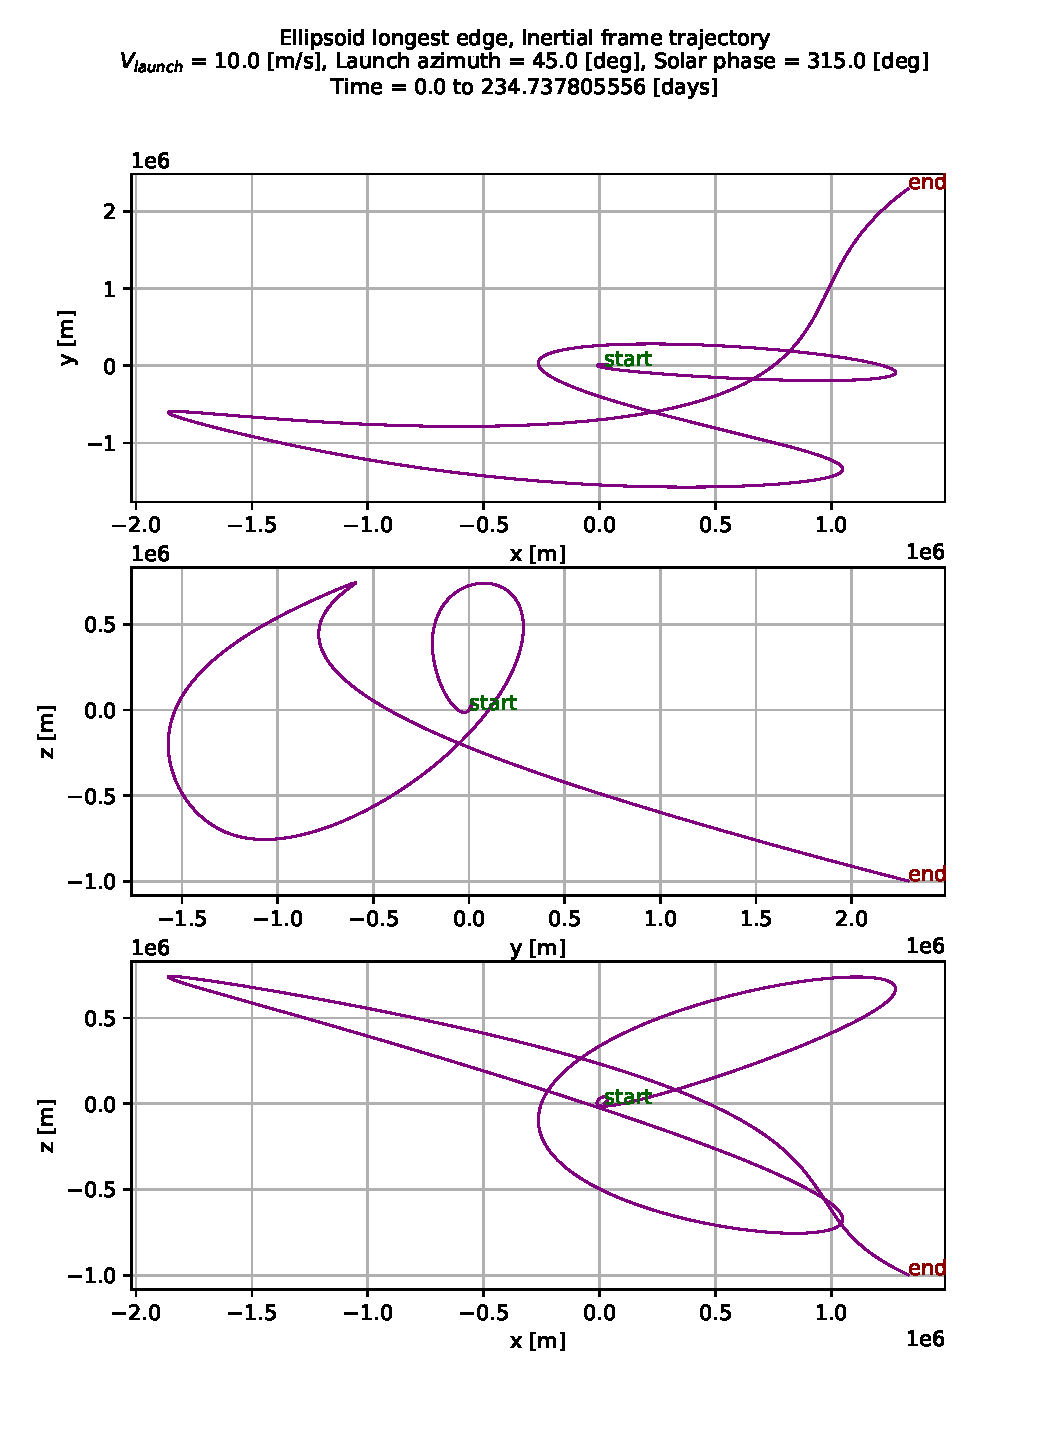
\includegraphics[angle=90, width=\linewidth, height=\textheight, keepaspectratio=true]{longest_edge_perturbations/3.2Density_1cmSize/10ms_45Azimuth_315SolarPhase/noSTBE_2d_trajectory_inertialFrame.pdf}
\caption{2D trajectory of particle for same initial conditions as that of capture case 5 in \Cref{tab:LoGSP_1_capture} except that only \gls{SRP} was included in this simulation. Particle code LoGSP-1.}
\label{fig:LoGSP_1_capture_case_5_2d_inertialTrajectory_noSTBE}
\end{figure}
\FloatBarrier
%%%
%%%
\begin{figure}[htb]
\centering
\captionsetup{justification=centering}
\subfloat[]{
    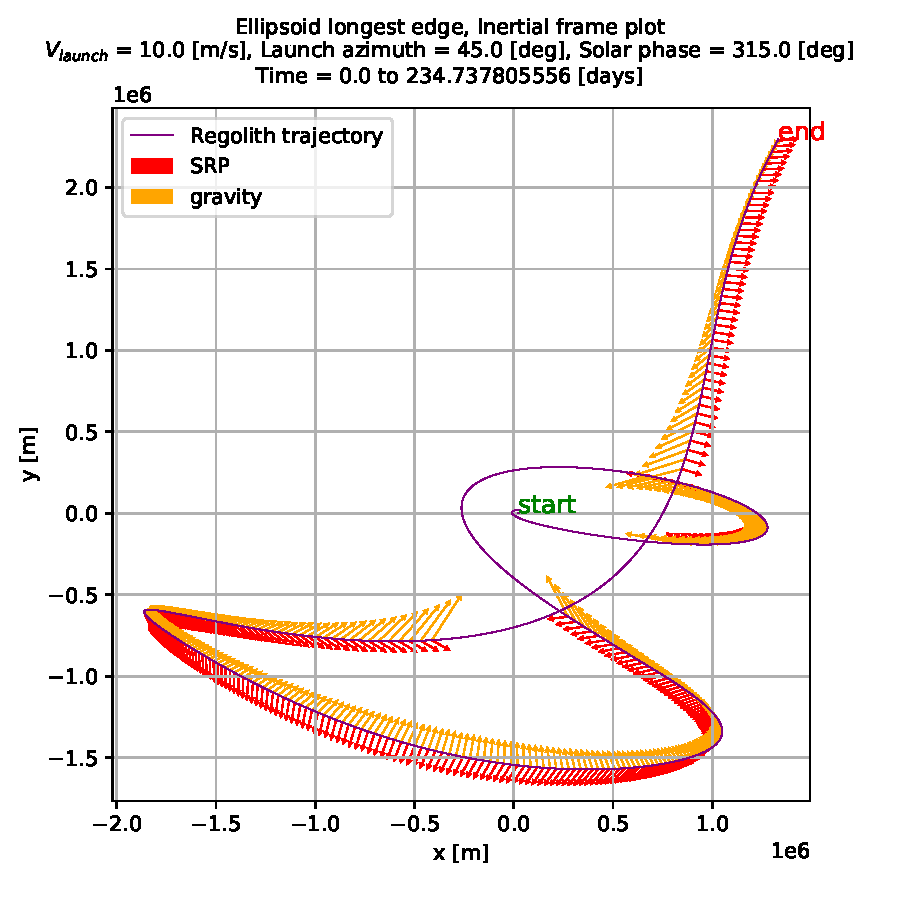
\includegraphics[width=0.5\linewidth, height=0.45\textheight, keepaspectratio=true]{longest_edge_perturbations/3.2Density_1cmSize/10ms_45Azimuth_315SolarPhase/noSTBE_srp_gravity_vectors_inertialFrame.pdf}
    \label{fig:LoGSP_1_capture_case_5_2d_SRP_and_gravity_vector_noSTBE_inertialFrame}
}
\subfloat[]{
    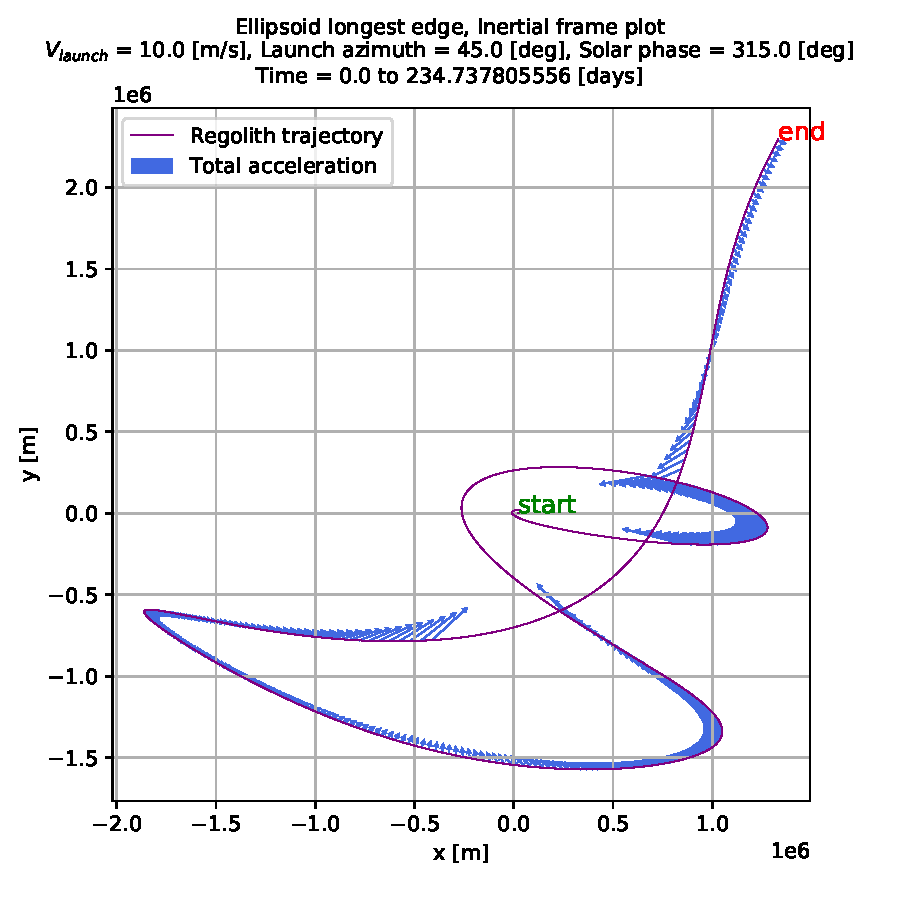
\includegraphics[width=0.5\linewidth, height=0.45\textheight, keepaspectratio=true]{longest_edge_perturbations/3.2Density_1cmSize/10ms_45Azimuth_315SolarPhase/noSTBE_total_acceleration_inertialFrame.pdf}
    \label{fig:LoGSP_1_capture_case_5_2d_totalAcceleration_vector_noSTBE_inertialFrame}
}
\caption{Inertial frame XY-plane trajectory for same launch conditions as that of capture case 5 in \Cref{tab:LoGSP_1_capture}: \protect\subref{fig:LoGSP_1_capture_case_5_2d_SRP_and_gravity_vector_noSTBE_inertialFrame} showing direction of \gls{SRP} acceleration and gravitational acceleration and \protect\subref{fig:LoGSP_1_capture_case_5_2d_totalAcceleration_vector_noSTBE_inertialFrame} showing direction of the net acceleration acting on the particle. Vectors are shown only for those parts of trajectory where acceleration due to \gls{SRP} and gravity have the same order of magnitude. Note that \gls{STBE} perturbation was not part of the simulation here. Particle code LoGSP-1.}
\end{figure}
\FloatBarrier
%%%

\subsubsection{Effects of omitting Solar Radiation Pressure (SRP)}
When we keep \gls{STBE} but remove \gls{SRP} from our simulations, the trajectory again leads to an escape situation, only this time much faster. The 2D inertial frame trajectory is shown in \Cref{fig:LoGSP_1_capture_case_5_2d_inertialTrajectory_noSRP}. The trajectory shows similarity only for a brief moment immediately after launch (notice the small loop after 'start') with the capture case in \Cref{fig:LoGSP_1_capture_case_5_2d_traj_inertialFrame}, but soon after the particle is on a trajectory that never comes back around the asteroid. The reason for this is clear and simple if one looks at the direction of acceleration due to gravity and \gls{STBE} in \Cref{fig:LoGSP_1_capture_case_5_2d_STBE_and_gravity_vector_noSRP_inertialFrame} and their net effect in \Cref{fig:LoGSP_1_capture_case_5_2d_totalAcceleration_vector_noSRP_inertialFrame}. Initially, from the point when we show these vectors, we know that the magnitude of \gls{STBE} acceleration is one order of magnitude smaller than the gravitational acceleration (see \Cref{fig:LoGSP_1_capture_case_5_2d_acceleration_magnitudes_noSRP}) and even then the direction of the net acceleration vector is such that the trajectory can not loop around the asteroid. The \gls{STBE} magnitude increases soon enough to the same order as that of gravitational acceleration and the net acceleration vector direction never points towards the asteroid which eventually causes the particle to escape. However, the point where the magnitude curves of \gls{STBE} and gravitational acceleration cross is not the point where the escape occurs as is evident from the plot for total energy and eccentricity in \Cref{fig:LoGSP_1_capture_case_5_eccentricity_energy_noSRP}.
%
\newline\newline
%
From this analysis, we can say that effect of removing \gls{SRP} from simulations had a much more drastic effect than removing just the \gls{STBE}. Both cases lead to an escape situation and the combined effect of both the perturbations leads to a capture orbit, for the same launch conditions and initial Solar phase angle. The behavior of the trajectory, in all cases, can be easily understood by looking at the direction of the net acceleration vector, especially when the particle is far away from the asteroid because it tells us exactly, how by adding perturbations, the motion of the particle is affected and not just in terms of its final fate but even in terms of changing its orbital direction.

\subsubsection{Capture Trajectory: Another Example}
\Cref{fig:LoGSP_1_capture_case_8_3d_traj_inertialFrame_differnetViews} shows the 3D trajectory for completely different launch conditions (see capture case 8 in \Cref{tab:LoGSP_1_capture}). The 3D trajectory as viewed in the \gls{ARF} is shown in \Cref{fig:LoGSP_1_capture_case_8_3d_trajectory}. The 2D trajectory projections for the same, in inertial and \gls{ARF}, are shown in \Cref{fig:LoGSP_1_capture_case_8_2d_traj_inertialFrame} and \Cref{fig:LoGSP_1_capture_case_8_2d_traj_bodyFrame} respectively. Just like in the previous case, we see from the animation (see \Cref{fig:LoGSP_1_capture_case_8_2d_trajectory_animation}) and the 3D trajectory for current launch conditions, that the particle direction of motion is reversed twice in its course. These two locations are marked by numbers 1 and 2 in \Cref{fig:LoGSP_1_capture_case_8_2d_traj_inertialFrame}. At location number 1 we see that the motion changes from anti-clockwise to clockwise direction in the XY-plane. The case for location number 2 is exactly the opposite. If we look at \Cref{fig:LoGSP_1_capture_case_8_2d_trajectory_totalPerturbationVectors}, the change in direction of motion is consistent with the direction in which the net perturbing force is acting. Ultimately, when we look at the net acceleration acting on the particle in \Cref{fig:LoGSP_1_capture_case_8_2d_totalAccelerationVector}, we can understand how exactly the particle would orbit around the asteroid. The net force, gravitational and perturbations combined, act in a direction such that the particle is forced to change its orbital motion direction at the two locations previously explained. The acceleration vectors in \Cref{fig:LoGSP_1_capture_case_8_2d_trajectory_perturbationVectors,fig:LoGSP_1_capture_case_8_2d_trajectory_totalPerturbations_and_gravity_vectors,fig:LoGSP_1_capture_case_8_2d_totalAccelerationVector} are plotted for points along the trajectory where the magnitude of acceleration due to \gls{SRP} is of the same order of magnitude as the gravitational acceleration. Again, the magnitude of \gls{STBE} is one order of magnitude smaller than the gravitational acceleration for the same data points along the trajectory.
%%%
\begin{figure}[htb]
\centering
\captionsetup{justification=centering}
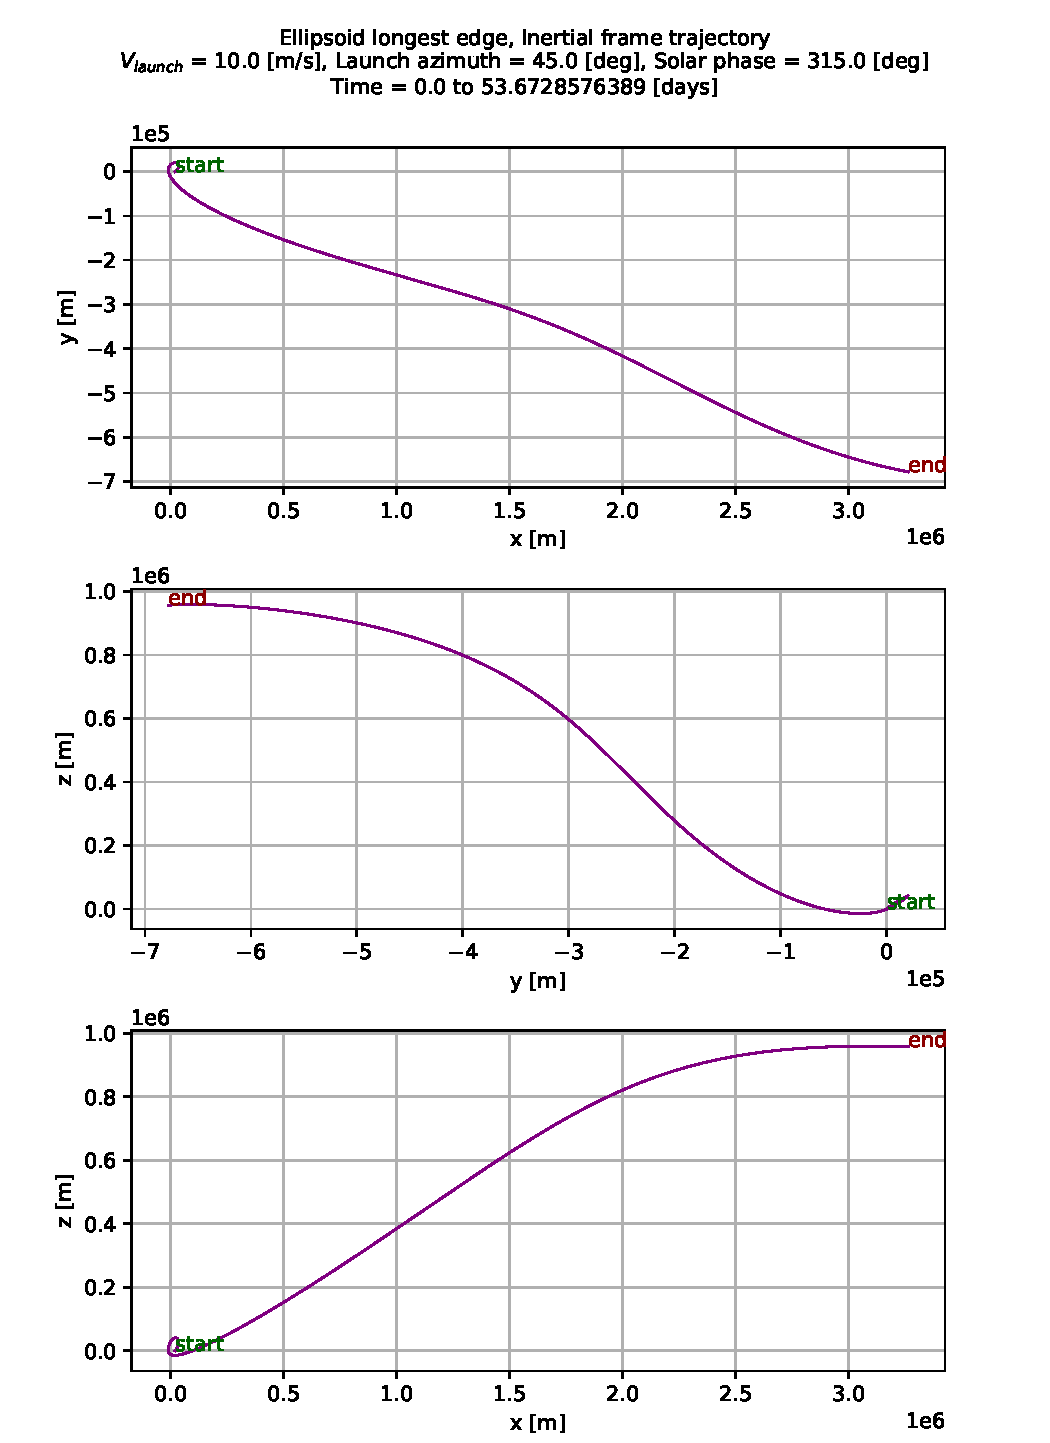
\includegraphics[angle=90, width=0.9\linewidth, height=\textheight, keepaspectratio=true]{longest_edge_perturbations/3.2Density_1cmSize/10ms_45Azimuth_315SolarPhase/noSRP_2d_trajectory_inertialFrame.pdf}
\caption{2D trajectory of particle for same initial conditions as that of capture case 5 in \Cref{tab:LoGSP_1_capture} except that only \gls{STBE} was included in this simulation. Particle code LoGSP-1.}
\label{fig:LoGSP_1_capture_case_5_2d_inertialTrajectory_noSRP}
\end{figure}
\FloatBarrier
%%%
%%%
\begin{figure}[htb]
\centering
\captionsetup{justification=centering}
\subfloat[]{
    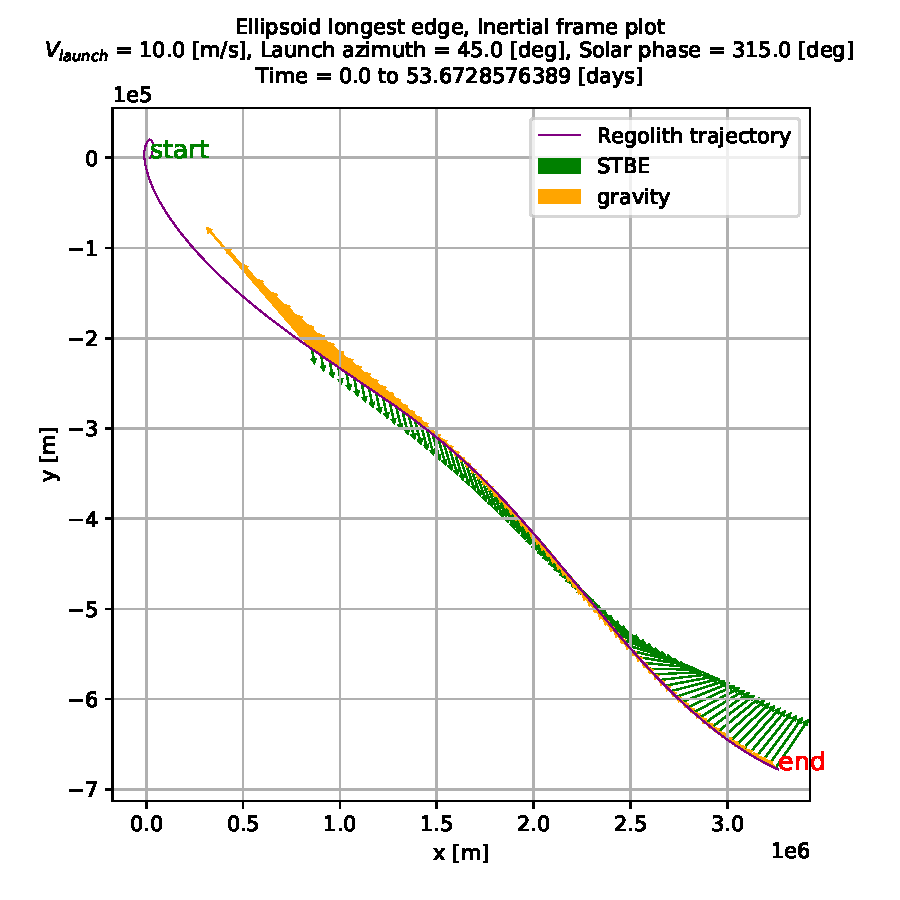
\includegraphics[width=0.5\linewidth, height=0.3\textheight, keepaspectratio=true]{longest_edge_perturbations/3.2Density_1cmSize/10ms_45Azimuth_315SolarPhase/noSRP_stbe_gravity_vectors_inertialFrame.pdf}
    \label{fig:LoGSP_1_capture_case_5_2d_STBE_and_gravity_vector_noSRP_inertialFrame}
}
\subfloat[]{
    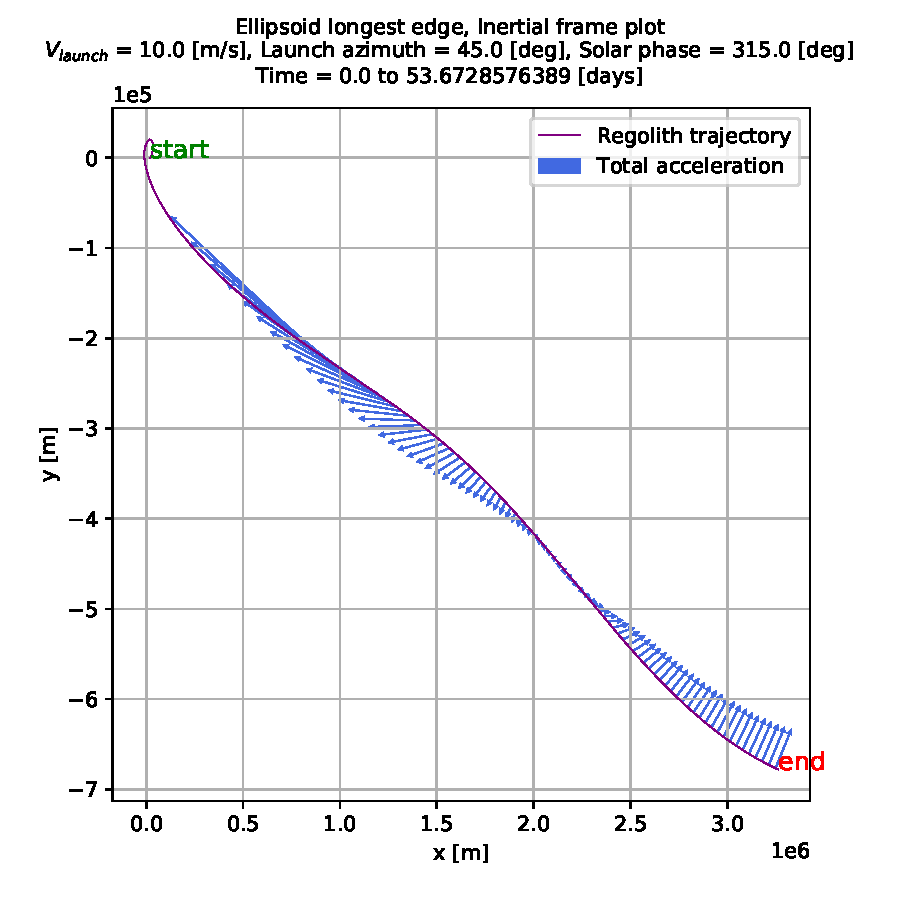
\includegraphics[width=0.5\linewidth, height=0.3\textheight, keepaspectratio=true]{longest_edge_perturbations/3.2Density_1cmSize/10ms_45Azimuth_315SolarPhase/noSRP_total_acceleration_inertialFrame.pdf}
    \label{fig:LoGSP_1_capture_case_5_2d_totalAcceleration_vector_noSRP_inertialFrame}
}
\caption{Inertial frame XY-plane trajectory for same launch conditions as that of capture case 5 in \Cref{tab:LoGSP_1_capture}: \protect\subref{fig:LoGSP_1_capture_case_5_2d_STBE_and_gravity_vector_noSRP_inertialFrame} showing direction of \gls{STBE} acceleration and gravitational acceleration and \protect\subref{fig:LoGSP_1_capture_case_5_2d_totalAcceleration_vector_noSRP_inertialFrame} showing direction of the net acceleration acting on the particle. Vectors are shown only for those parts of trajectory where acceleration due to \gls{STBE} is equal to gravitational acceleration or smaller than it by one order of magnitude. Note that \gls{SRP} perturbation was not part of the simulation here. Particle code LoGSP-1.}
\label{fig:LoGSP_1_capture_case_5_2d_noSRP_accelerationVectorPlot_inertialFrame}
\end{figure}
\FloatBarrier
%%%
%%%
\begin{figure}[htb]
\centering
\captionsetup{justification=centering}
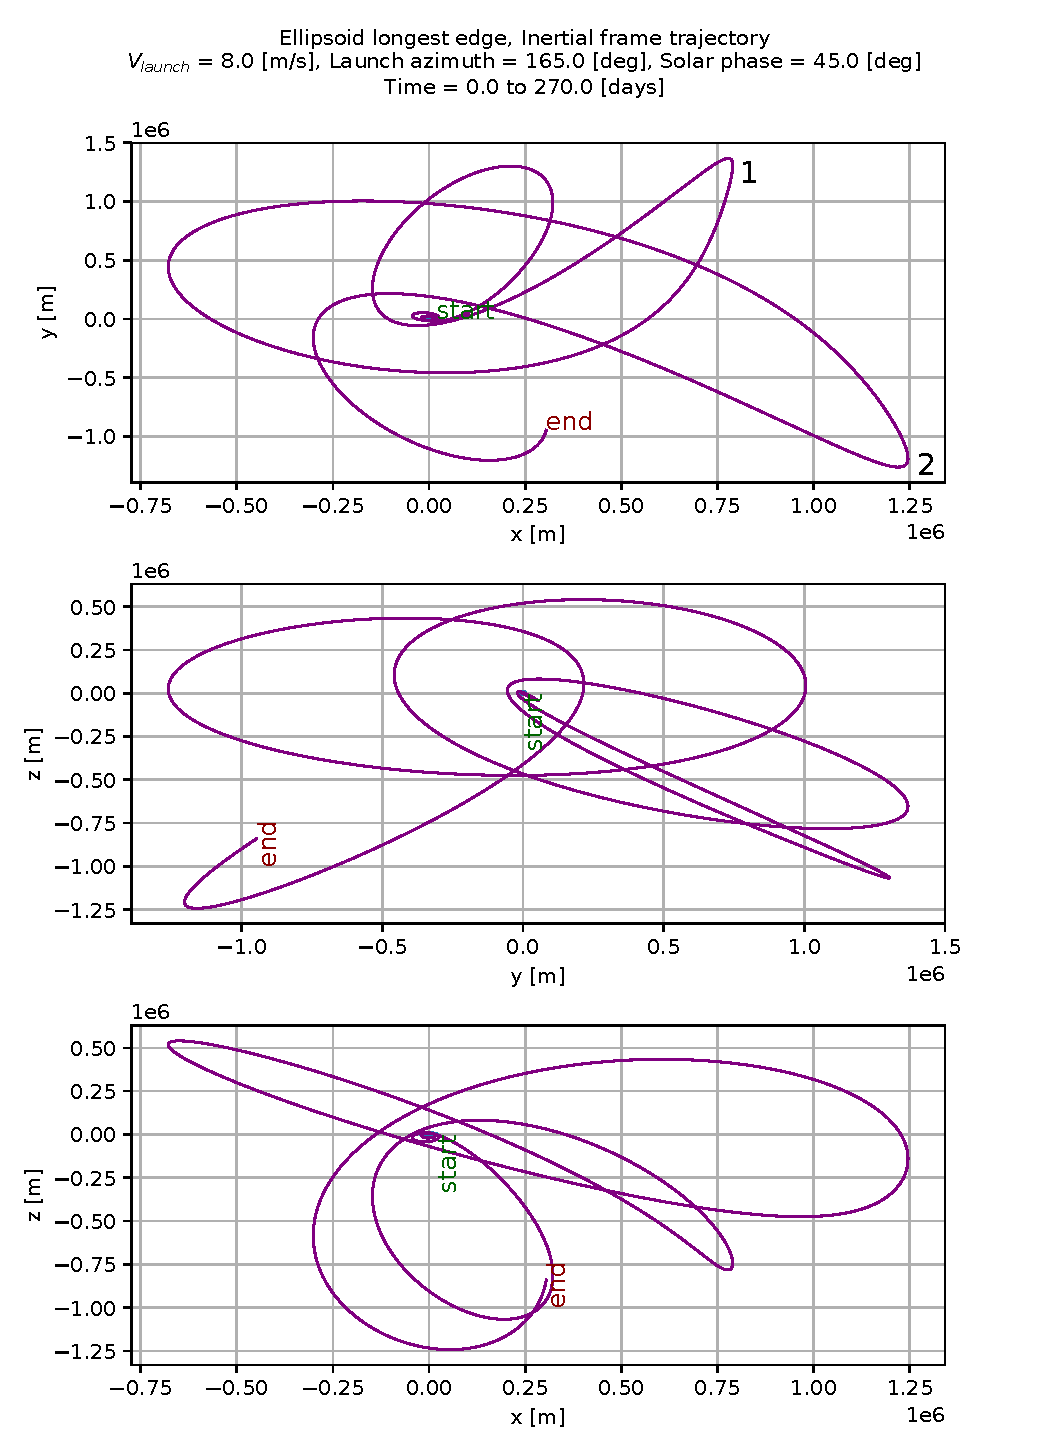
\includegraphics[angle=90, width=\textwidth, height=\textheight, keepaspectratio=true]{longest_edge_perturbations/3.2Density_1cmSize/2dTrajectory_8ms_165Azimuth_45solarPhase_inertialFrame_edit.pdf}
\caption{2D inertial frame trajectory of capture regolith for case number 8 in \Cref{tab:LoGSP_1_capture}. Particle code LoGSP-1.}
\label{fig:LoGSP_1_capture_case_8_2d_traj_inertialFrame}
\end{figure}
\FloatBarrier
%%%
%%%
\begin{figure}[!h]
\centering
\captionsetup{justification=centering}
\subfloat[]{
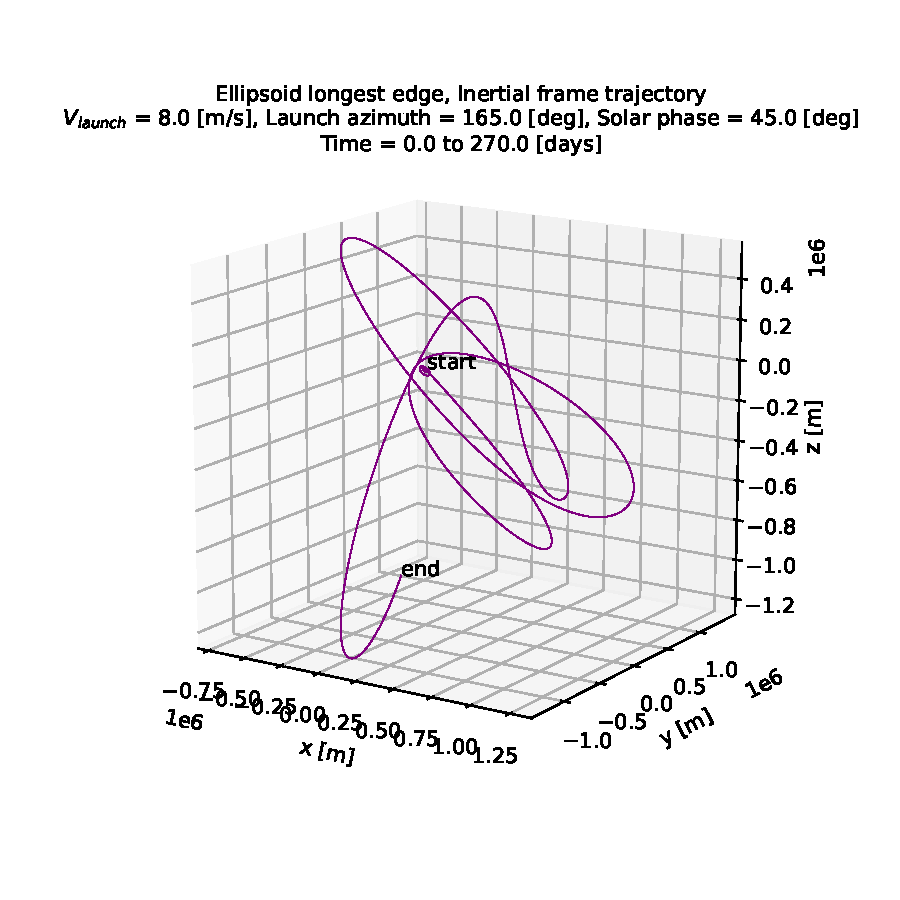
\includegraphics[width=0.5\textwidth, height=0.5\textheight, keepaspectratio=true]{longest_edge_perturbations/3.2Density_1cmSize/3dTrajectory_8ms_165Azimuth_45solarPhase_inertialFrame_View1.pdf}
}
\subfloat[]{
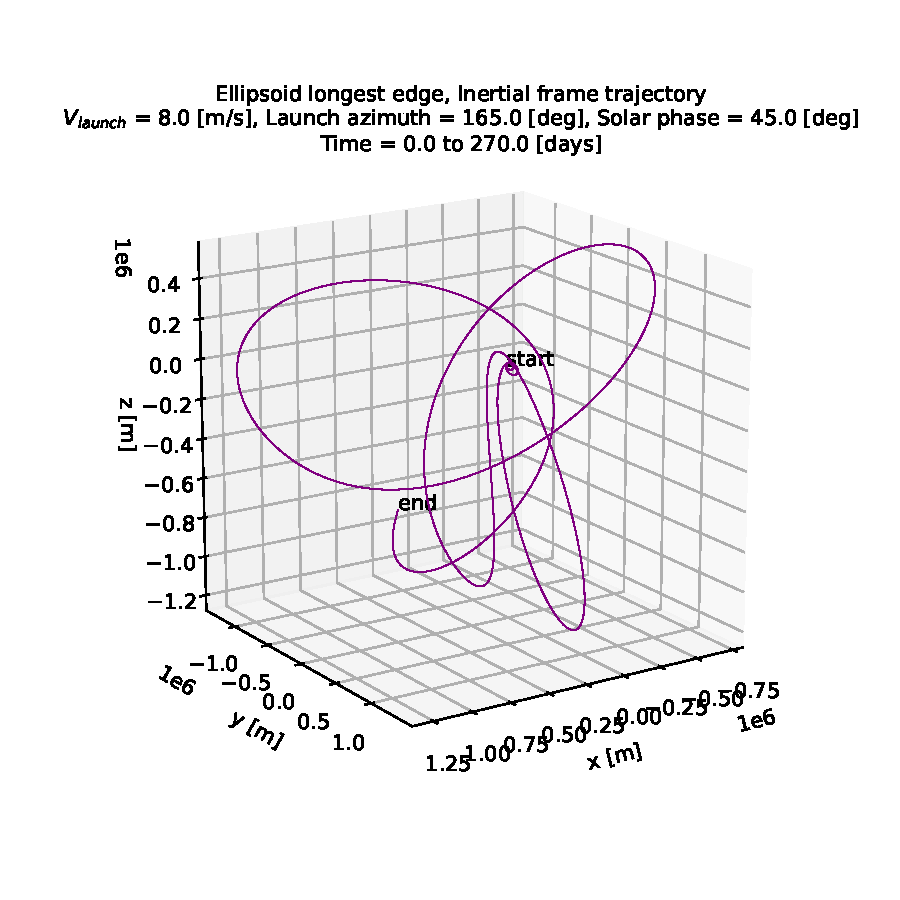
\includegraphics[width=0.5\textwidth, height=0.5\textheight, keepaspectratio=true]{longest_edge_perturbations/3.2Density_1cmSize/3dTrajectory_8ms_165Azimuth_45solarPhase_inertialFrame_View2.pdf}
}
\caption{3D inertial frame trajectory of capture regolith for case number 8 in \Cref{tab:LoGSP_1_capture} from two different viewing angles. Particle code LoGSP-1.}
\label{fig:LoGSP_1_capture_case_8_3d_traj_inertialFrame_differnetViews}
\end{figure}
\FloatBarrier
%%%
%%%
\begin{figure}[htb]
\centering
\captionsetup{justification=centering}
% another option for includegraphics - keepaspectratio
\subfloat[]{
    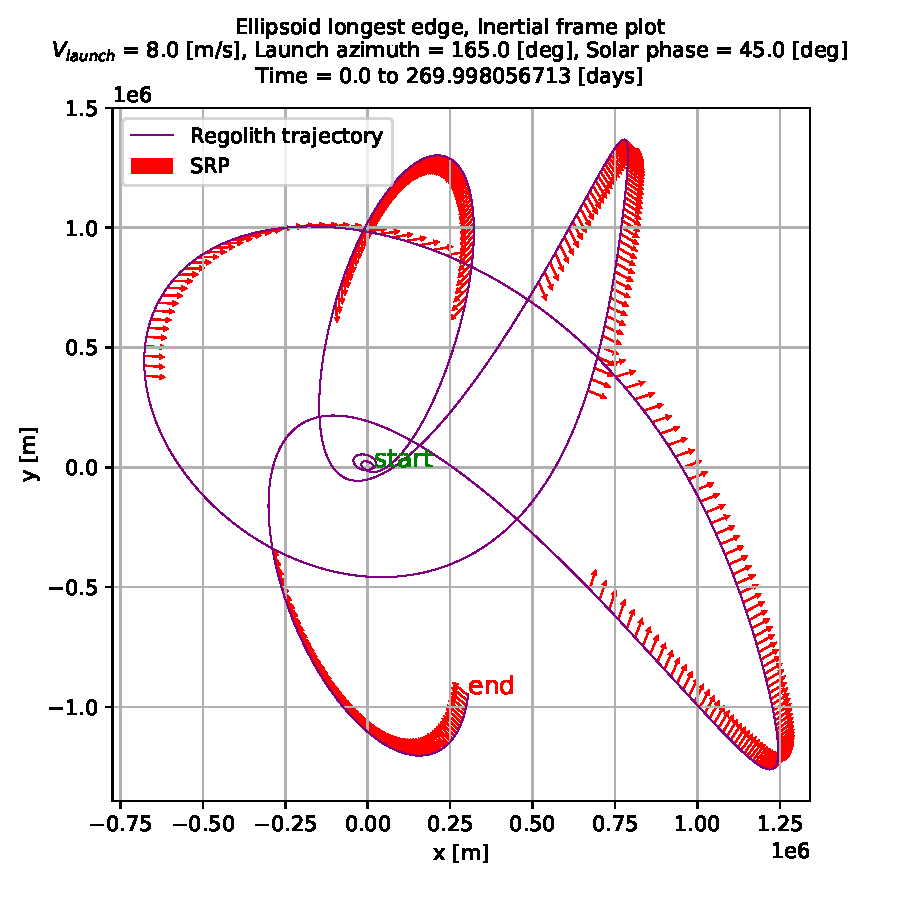
\includegraphics[width=0.5\linewidth, height=0.45\textheight, keepaspectratio=true]{longest_edge_perturbations/3.2Density_1cmSize/8ms_165Azimuth_45SolarPhase/srp_vectors.pdf}
    \label{fig:LoGSP_1_capture_case_8_2d_trajectory_srp_vectors}
}
\subfloat[]{
    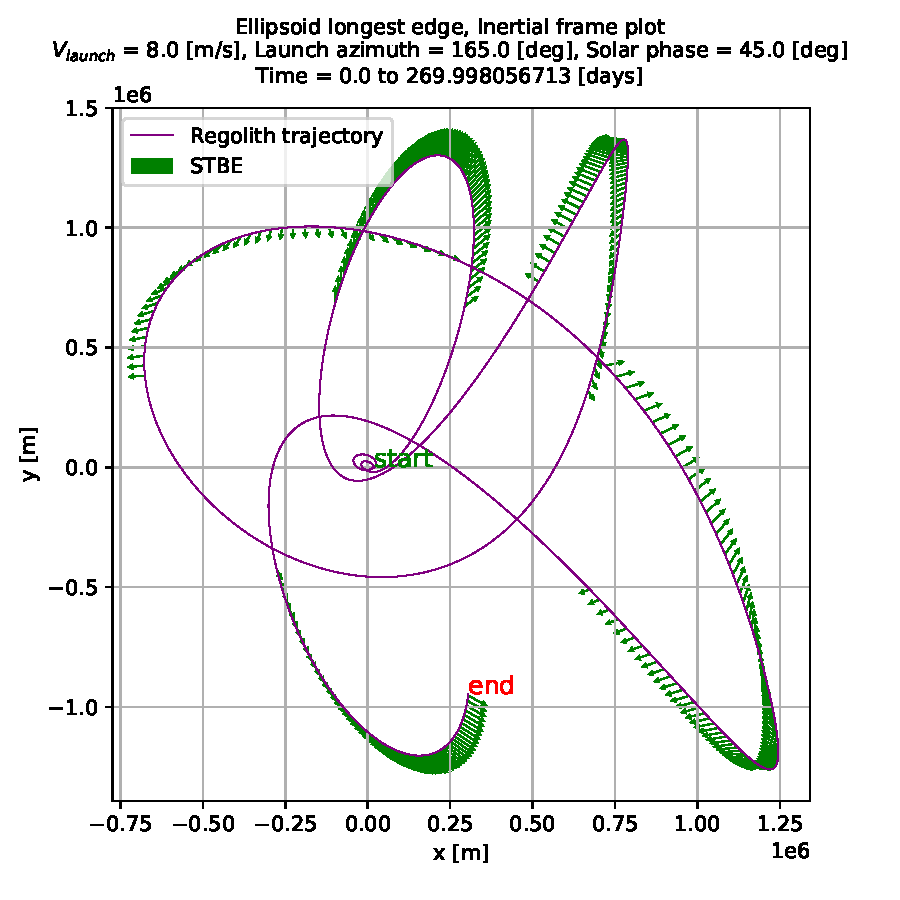
\includegraphics[width=0.5\linewidth, height=0.45\textheight, keepaspectratio=true]{longest_edge_perturbations/3.2Density_1cmSize/8ms_165Azimuth_45SolarPhase/stbe_vectors.pdf}
    \label{fig:LoGSP_1_capture_case_8_2d_trajectory_stbe_vectors}
}
\caption{2D trajectory of capture regolith for case number 8 in \Cref{tab:LoGSP_1_capture} with direction of \gls{SRP} and \gls{STBE} perturbation vectors. Note that the vectors are shown only for those parts of the trajectory where the \gls{SRP} magnitude is of the same order as that of the asteroid's gravitational acceleration. For those very same points along the trajectory, the magnitude of the \gls{STBE} is always one order of magnitude smaller than the gravitational acceleration. Particle code LoGSP-1.}
\label{fig:LoGSP_1_capture_case_8_2d_trajectory_perturbationVectors}
\end{figure}
\FloatBarrier
%%%
%%%
\begin{figure}[htb]
\centering
\captionsetup{justification=centering}
\subfloat[]{
    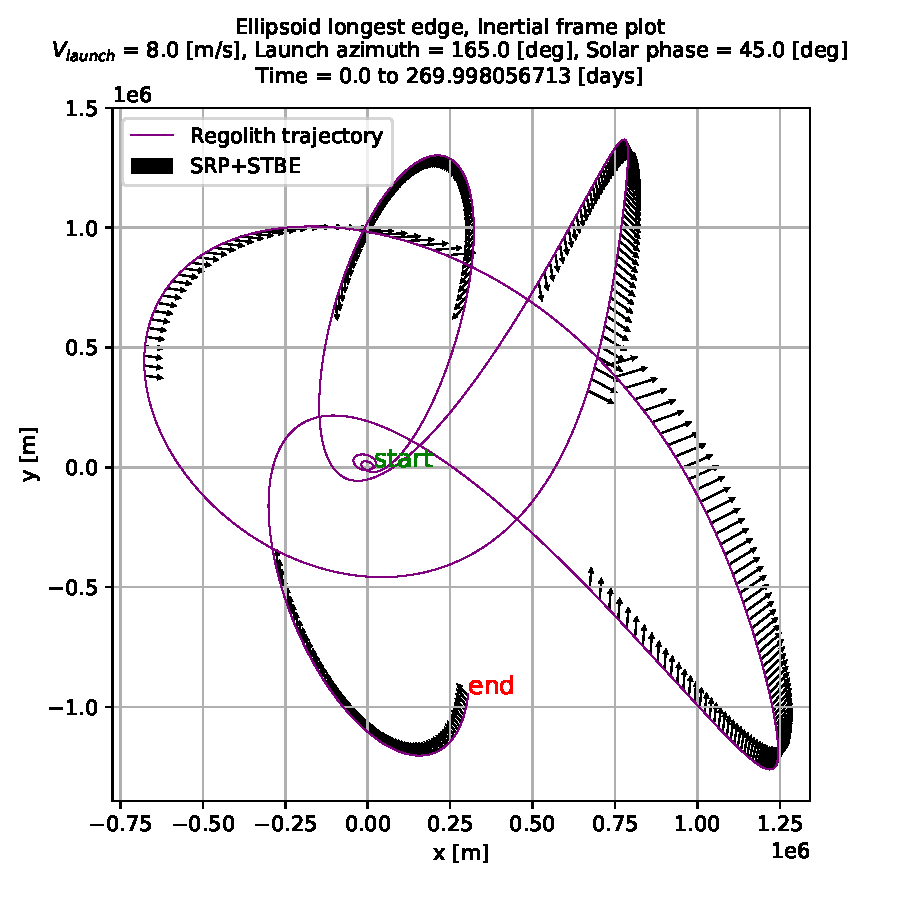
\includegraphics[width=0.5\linewidth, height=0.45\textheight, keepaspectratio=true]{longest_edge_perturbations/3.2Density_1cmSize/8ms_165Azimuth_45SolarPhase/netPerturbations_vectors.pdf}
    \label{fig:LoGSP_1_capture_case_8_2d_trajectory_totalPerturbationVectors}
}
\subfloat[]
{
    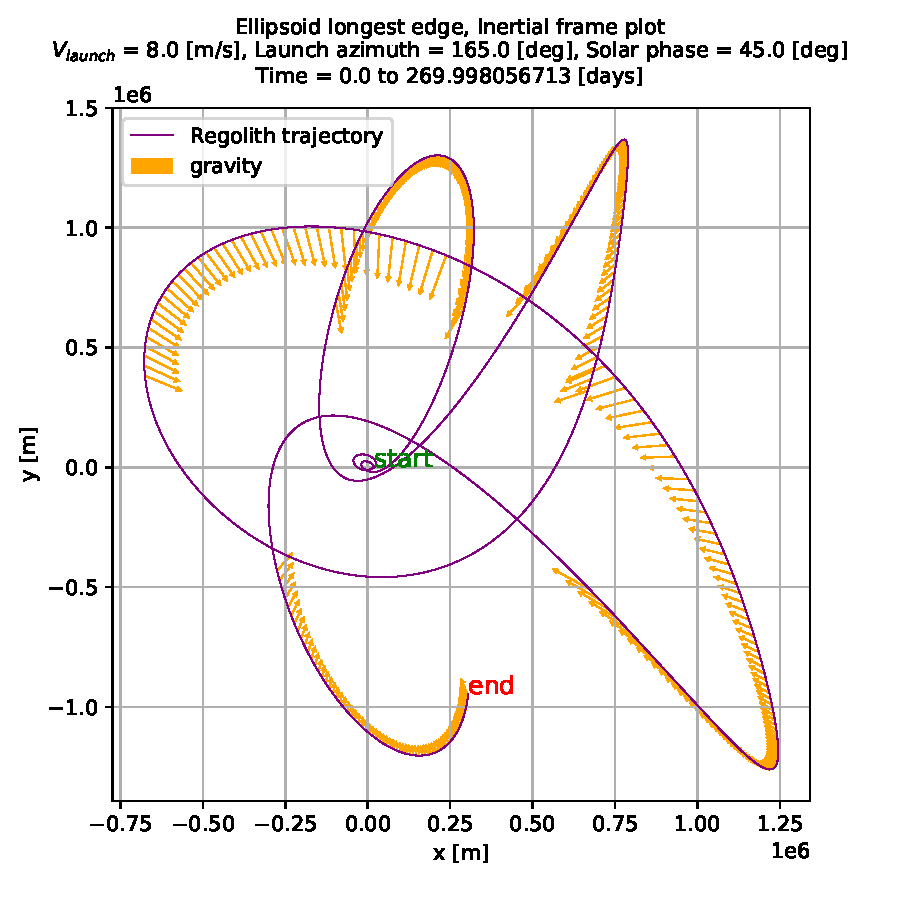
\includegraphics[width=0.5\linewidth, height=0.45\textheight, keepaspectratio=true]{longest_edge_perturbations/3.2Density_1cmSize/8ms_165Azimuth_45SolarPhase/gravity_vectors.pdf}
    \label{fig:LoGSP_1_capture_case_8_2d_trajectory_gravityVector}
}
\caption{2D trajectory of capture regolith for case number 8 in \Cref{tab:LoGSP_1_capture} with direction of the sum total of \gls{SRP} and \gls{STBE} perturbation vectors, and the direction of the gravitational acceleration vector for the same data points. Note that the vectors are shown only for those parts of the trajectory where the \gls{SRP} magnitude is of the same order as that of the asteroid's gravitational acceleration. For those very same points along the trajectory, the magnitude of the \gls{STBE} is always one order of magnitude smaller than the gravitational acceleration. Particle code LoGSP-1.}
\label{fig:LoGSP_1_capture_case_8_2d_trajectory_totalPerturbations_and_gravity_vectors}
\end{figure}
\FloatBarrier
%%%
%%%
\begin{figure}[htb]
\centering
\captionsetup{justification=centering}
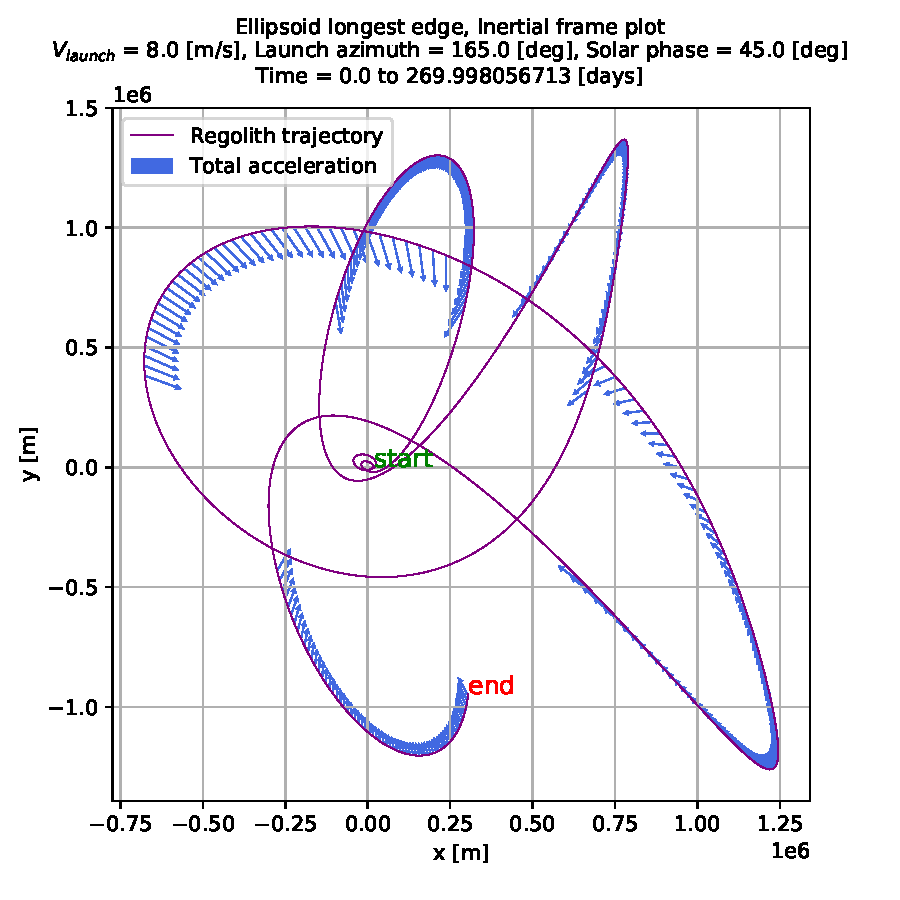
\includegraphics[width=\linewidth, height=0.45\textheight, keepaspectratio=true]{longest_edge_perturbations/3.2Density_1cmSize/8ms_165Azimuth_45SolarPhase/netAcceleration_vectors.pdf}
\caption{2D trajectory of capture regolith for case number 8 in \Cref{tab:LoGSP_1_capture} with direction of the net acceleration vector. Note that the vectors are shown only for those parts of the trajectory where the \gls{SRP} magnitude is of the same order as that of the asteroid's gravitational acceleration. For those very same points along the trajectory, the magnitude of the \gls{STBE} is always one order of magnitude smaller than the gravitational acceleration. Particle code LoGSP-1.}
\label{fig:LoGSP_1_capture_case_8_2d_totalAccelerationVector}
\end{figure}
\FloatBarrier
%%%
%%%
\begin{figure}[htb]
\centering
\captionsetup{justification=centering}
% another option for includegraphics - keepaspectratio

\includegraphics[scale=0.25]{longest_edge_perturbations/3.2Density_1cmSize/qrcode_8ms_165Azimuth_45SolarPhase.png}
\caption{2D trajectory animation (XY-Plane) of capture regolith for case number 8 in \Cref{tab:LoGSP_1_capture}. Particle code LoGSP-1. Scan the QR code to view the animation or use the following web-link: \url{https://youtu.be/CceYRlNvAiM}}
\label{fig:LoGSP_1_capture_case_8_2d_trajectory_animation}
\end{figure}
\FloatBarrier
%%%

\subsubsection{Formation of capture orbits}
We saw in the analysis of capture case number 5 for particle LoGSP-1 that both \gls{SRP} and \gls{STBE} were necessary for getting that specific capture trajectory and removal of either of the perturbations resulted in a different final fate for the same particle. The next analysis that we present now, will tell us about how a capture scenario occurs, relative to a situation when all perturbations are removed, for the same initial launch conditions in both cases. We do the analysis for capture case number 8 from \Cref{tab:LoGSP_1_capture}. \Cref{fig:LoGSP_1_capture_case_8_2d_trajectory_comparative_inertialFrame} shows two different trajectories for the particle launched with the same initial conditions. The one shown in dotted line is for the case when Solar perturbations were omitted from the simulation, which eventually results in the particle escaping the asteroid after 1.4 days. The one in the solid line shows the capture trajectory (actually a section of the entire capture trajectory as seen in \Cref{fig:LoGSP_1_capture_case_8_2d_traj_inertialFrame}) when Solar perturbations were included in the simulation. Note that we show the perturbed trajectory (capture case) for the same amount of time (1.4 days instead of 270.0 days) as taken by the unperturbed trajectory (escape case) to be able to do a one-to-one comparison. The arrows plotted along this trajectory indicate the direction of the net perturbing acceleration due to \gls{SRP} and \gls{STBE}. \Cref{fig:LoGSP_1_capture_case_8_2d_trajectory_comparative_animation} directs to an animation for both the unperturbed and perturbed trajectory.
%%%
\begin{figure}[htb]
\centering
\captionsetup{justification=centering}
% another option for includegraphics - keepaspectratio

\includegraphics[scale=0.25]{longest_edge_perturbations/3.2Density_1cmSize/qrcode_comparative_8ms_165Azimuth_45SolarPhase.png}
\caption{2D trajectory animation (XY-Plane) of capture regolith for case number 8 in \Cref{tab:LoGSP_1_capture}, compared with that of its unperturbed counterpart. Particle code LoGSP-1. Scan the QR code to view the animation or use the following web-link: \url{https://youtu.be/CdFKKR3UDJ0}}
\label{fig:LoGSP_1_capture_case_8_2d_trajectory_comparative_animation}
\end{figure}
\FloatBarrier
%%%
From the animation we can see that even as the particle has just been lofted from the surface of the asteroid, there are very subtle and minute differences in the range to the particle and its velocity, between the perturbed and unperturbed trajectory. The first visible difference between the two trajectories becomes noticeable at point \textit{"A"} in \Cref{fig:LoGSP_1_capture_case_8_2d_trajectory_comparative_inertialFrame}. It is easy to deduce the change in the perturbed trajectory from the direction of the net perturbing acceleration up until this point. The same point \textit{"A"} is also marked in \Cref{fig:LoGSP_1_capture_case_8_comparative_total_energy}. It is from this point that we can see noticeable difference between the two trajectories as well as in their corresponding energies. A snippet from the trajectory animation, corresponding to the point \textit{"A"}, is shown in \Cref{fig:LoGSP_1_capture_case_8_2d_comparative_animation_snippet} which highlights the differences in range and velocity of the particles in the two trajectories. Note that in \Cref{fig:LoGSP_1_capture_case_8_2d_comparative_animation_snippet}, the difference in the velocity between the perturbed and unperturbed cases is relatively small, compared to almost \SI{1}{\kilo\metre} of a difference in range of the particles. The latter is significant since the particles have dimensions in the order of \si{\centi\metre}. From point \textit{"A"} onwards these differences continue to grow and only get larger as the trajectory proceeds.
%
\newline\newline
%
Similarly, at point \textit{"B"} in \Cref{fig:LoGSP_1_capture_case_8_2d_trajectory_comparative_inertialFrame}, we see a much larger difference between the two trajectories. In \Cref{fig:LoGSP_1_capture_case_8_comparative_total_energy}, we see that around point \textit{"B"} both trajectories have a positive energy which quickly comes down to a negative value for the perturbed trajectory, hence keeping it bounded which results in a capture scenario. However, this does not happen for the unperturbed trajectory, leading to an escape scenario. The difference in the state of the two particles at point \textit{"B"} is relatively larger and can be seen in \Cref{fig:LoGSP_1_capture_case_8_2d_comparative_animation_phasingExample}. The differences in the two trajectories, computed in the asteroid centric rotating frame, is shown in \Cref{fig:LoGSP_1_capture_case_8_2d_trajectory_comparative_bodyFrame}. The plot on the bottom shows the trajectory for 1.4 days (i.e. until escape for the unperturbed trajectory) as viewed in the rotating frame, and the plot on the right zooms into a small part of this trajectory to show how Solar perturbations are responsible for changing the course of the particle. It is seen with a bit more clarity on how the net perturbation vector pulls the trajectory away from the trace of the unperturbed one.
%
\newline\newline
%
So what we are seeing here is, that due to the inclusion of perturbations from the Sun, the motion of the particle changed with respect to its unperturbed counterpart. This change was not drastic in terms of the initial shape of the trajectory as seen in \Cref{fig:LoGSP_1_capture_case_8_2d_trajectory_comparative_inertialFrame}. But the change was just enough for the particle to have a different phase with respect to the asteroid, relative to the unperturbed trajectory as seen in \Cref{fig:LoGSP_1_capture_case_8_comparative_animation_snapshots}. By phase, we refer to the location of the particle with respect to a given rotational state of the asteroid. So if two particles are at different locations, at any given epoch and for the same rotational state of the asteroid, they will have different magnitudes of forces acting on them which would ultimately lead to different final outcomes.
%%%
\begin{figure}[htb]
\centering
\captionsetup{justification=centering}
\subfloat[]{
    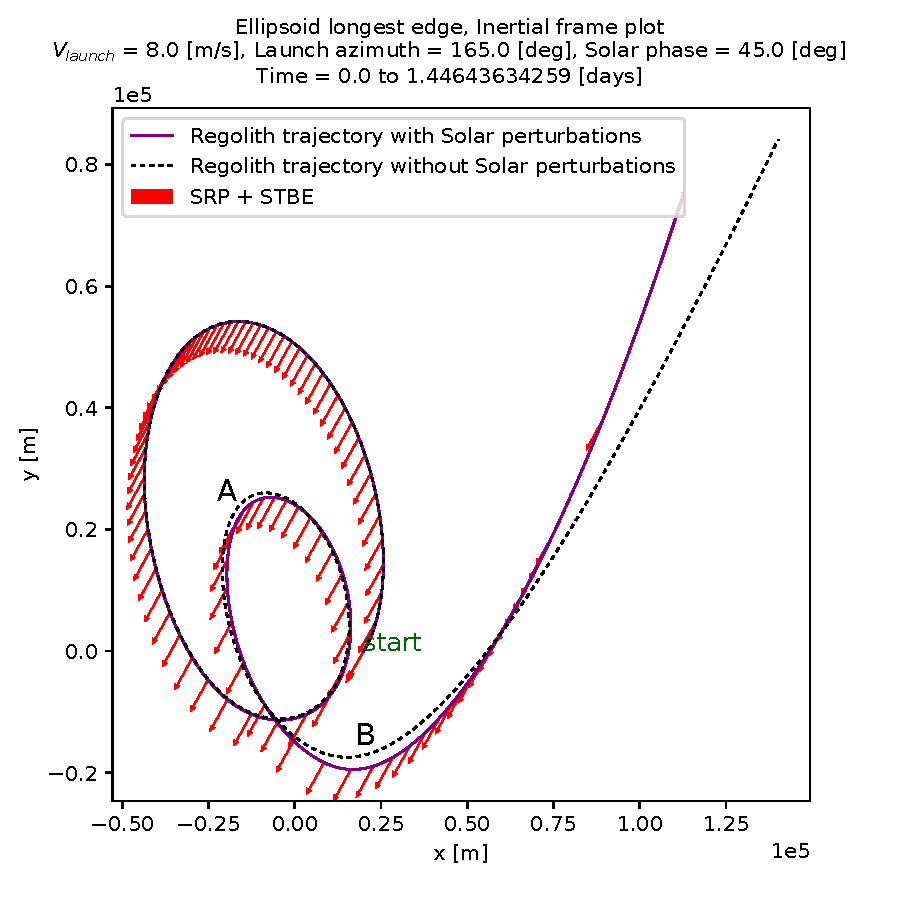
\includegraphics[width=\textwidth, height=0.45\textheight, keepaspectratio=true]{longest_edge_perturbations/3.2Density_1cmSize/8ms_165Azimuth_45SolarPhase/comparative_analysis_allPerturbations_inertialFrame_edit.pdf}
    \label{fig:LoGSP_1_capture_case_8_2d_trajectory_comparative_inertialFrame}
    % \caption{Inertial frame 2D trajectory (XY-plane) of capture regolith for case number 8 in \Cref{tab:LoGSP_1_capture} with direction of the net perturbation vector, compared with the trajectory of a particle launched with the same initial conditions but in absence of all Solar perturbations. Vectors are shown after a constant interval of 100 data points. Particle code LoGSP-1.}
}

\subfloat[]{
    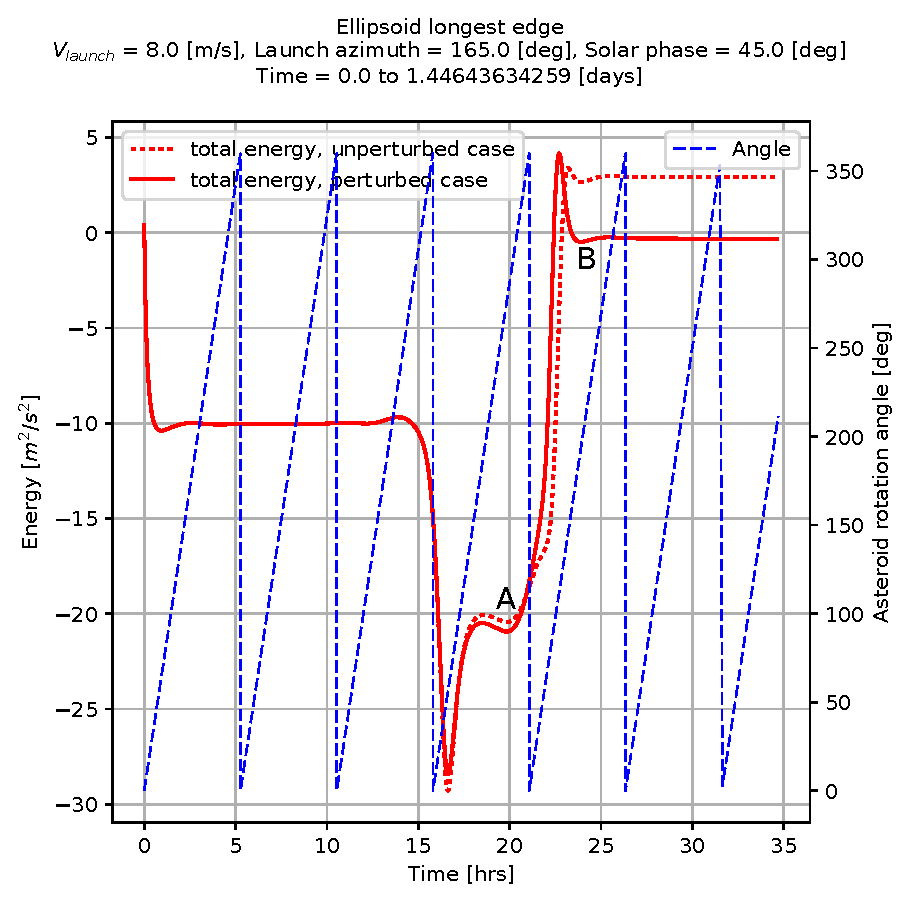
\includegraphics[width=\textwidth, height=0.45\textheight, keepaspectratio=true]{longest_edge_perturbations/3.2Density_1cmSize/8ms_165Azimuth_45SolarPhase/comparative_analysis_total_energy_edit.pdf}
    \label{fig:LoGSP_1_capture_case_8_comparative_total_energy}
    % \caption{Total energy plot for capture case number 8 in \Cref{tab:LoGSP_1_capture} compared with that of a particle launched with the same initial conditions but in absence of all Solar perturbations. Particle code LoGSP-1.}
}
\caption{Comparative analysis of capture case 8 in \Cref{tab:LoGSP_1_capture} with a particle trajectory where the initial conditions are same as the former but the simulation was done without Solar perturbations. \Cref{fig:LoGSP_1_capture_case_8_2d_trajectory_comparative_inertialFrame} compares the XY-plane trajectory and \Cref{fig:LoGSP_1_capture_case_8_comparative_total_energy} compares their total energy. Particle code LoGSP-1.}
\label{fig:LoGSP_1_capture_case_8_comparative analysis_trajectory_and_energy}
\end{figure}
\FloatBarrier
%%%
%%%
\begin{figure}[htb]
\centering
\captionsetup{justification=centering}
% another option for includegraphics - keepaspectratio
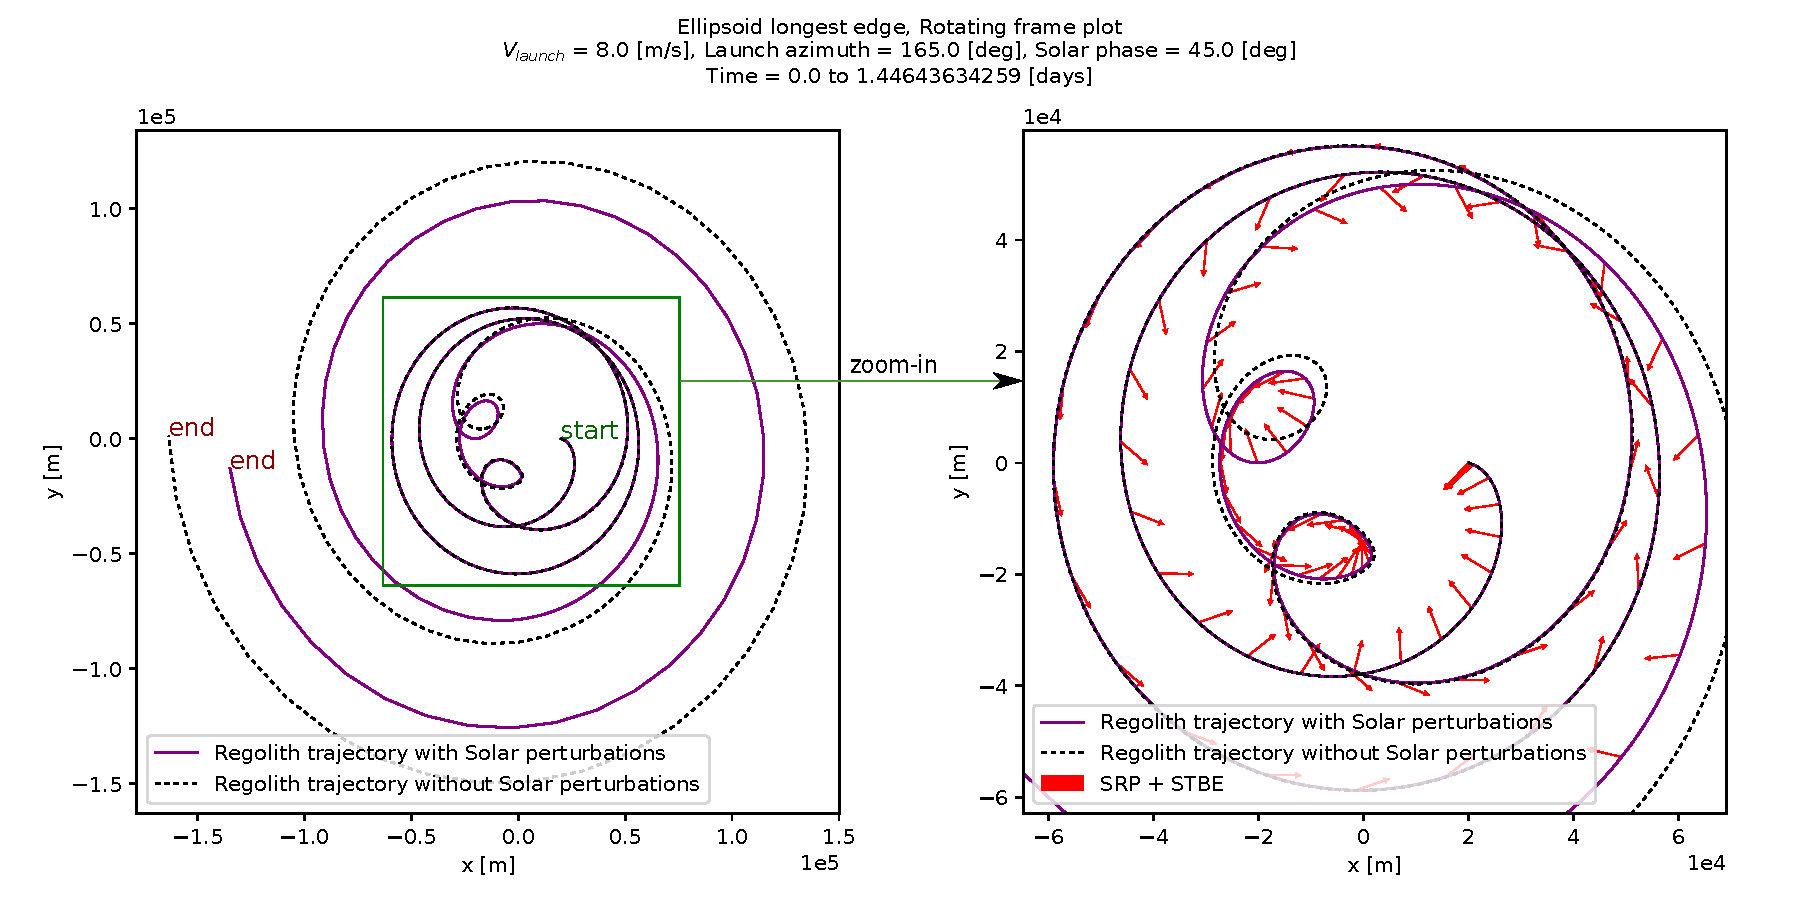
\includegraphics[angle=90, width=\textwidth, height=\textheight, keepaspectratio=true]{longest_edge_perturbations/3.2Density_1cmSize/8ms_165Azimuth_45SolarPhase/comparative_analysis_allPerturbations_rotatingFrame_edited.pdf}
\caption{Rotating frame 2D trajectory (XY-plane) of capture regolith for case number 8 in \Cref{tab:LoGSP_1_capture} with direction of the net perturbation vector, compared with the trajectory of a particle launched with the same initial conditions but in absence of Solar perturbations. Particle code LoGSP-1.}
\label{fig:LoGSP_1_capture_case_8_2d_trajectory_comparative_bodyFrame}
\end{figure}
\FloatBarrier
%%%
%%%
\begin{figure}[htb]
\centering
\captionsetup{justification=centering}
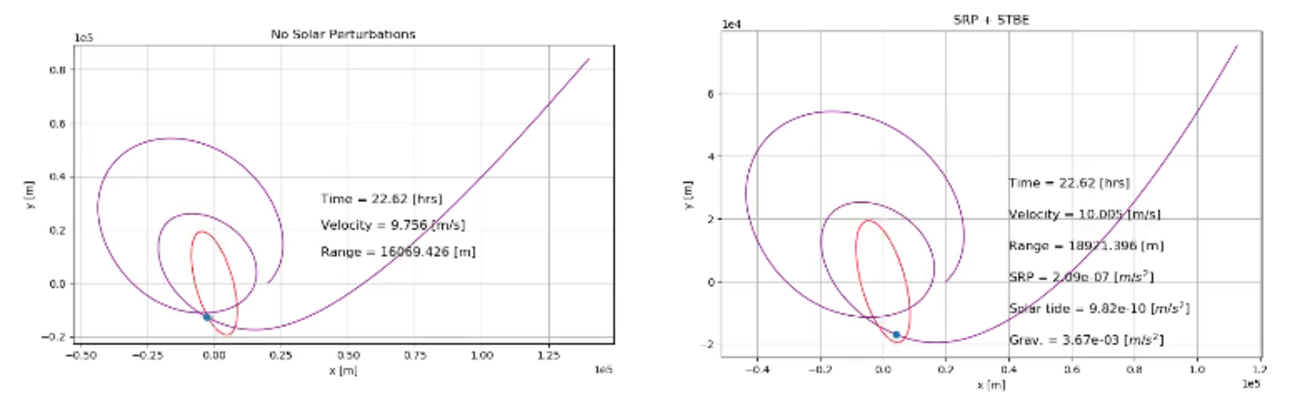
\includegraphics[angle=90, width=\textwidth, height=\textheight, keepaspectratio=true]{longest_edge_perturbations/3.2Density_1cmSize/8ms_165Azimuth_45SolarPhase/comparative_analysis_allPerturbations_phasing_animation_example.pdf}
\caption{Snapshot from animation of the perturbed trajectory of capture case 8 in \Cref{tab:LoGSP_1_capture} compared with that of its unperturbed counterpart. The unperturbed trajectory is still being accelerated at the given instant however the particle in the perturbed trajectory is being decelerated. Particle code LoGSP-1.}
\label{fig:LoGSP_1_capture_case_8_2d_trajectory_comparative_animation_phasing_snapshot}
\end{figure}
\FloatBarrier
%%%
If we look at the trajectory animation in \Cref{fig:LoGSP_1_capture_case_8_2d_trajectory_comparative_animation}, one would notice that at around point \textit{"B"}, the particle in the unperturbed trajectory is being accelerated by the gravitational pull of the asteroid while the particle in the perturbed trajectory is being slowed down. A snapshot of this scenario from the animation is shown in \Cref{fig:LoGSP_1_capture_case_8_2d_trajectory_comparative_animation_phasing_snapshot}. Although this situation does not happen for extended periods of time, but only while approaching point \textit{"B"}, we see that the particle in the unperturbed trajectory has a relatively higher velocity while moving forth of point \textit{"B"} and leaving the vicinity of the asteroid, relative to the particle in the perturbed trajectory. The latter thus stays in a capture orbit while the former has enough velocity to escape. A plot for this is shown in \Cref{fig:LoGSP_1_capture_case_8_comparative_inertial_velocity}.
%
\newline\newline
%
Note that in the capture case just discussed, the magnitude of the perturbing accelerations is much smaller than the gravitational acceleration. The effect of the perturbations on the particle's trajectory is not instantaneous and we can see that in the initial part of the trajectories up until point \textit{"A"} in \Cref{fig:LoGSP_1_capture_case_8_2d_trajectory_comparative_inertialFrame}. Until this point, acceleration due to gravity is in the order of $10^{-4}$, while accelerations due to \gls{SRP} and \gls{STBE} are in the orders of $10^{-7}$ and $10^{-9}$ respectively. Although the perturbing magnitudes are small, the particles in question are extremely small as well and so over time, the perturbing accelerations add up, leading to a significant change in the trajectory from the unperturbed one.
%%%
\begin{figure}[htb]
\centering
\captionsetup{justification=centering}
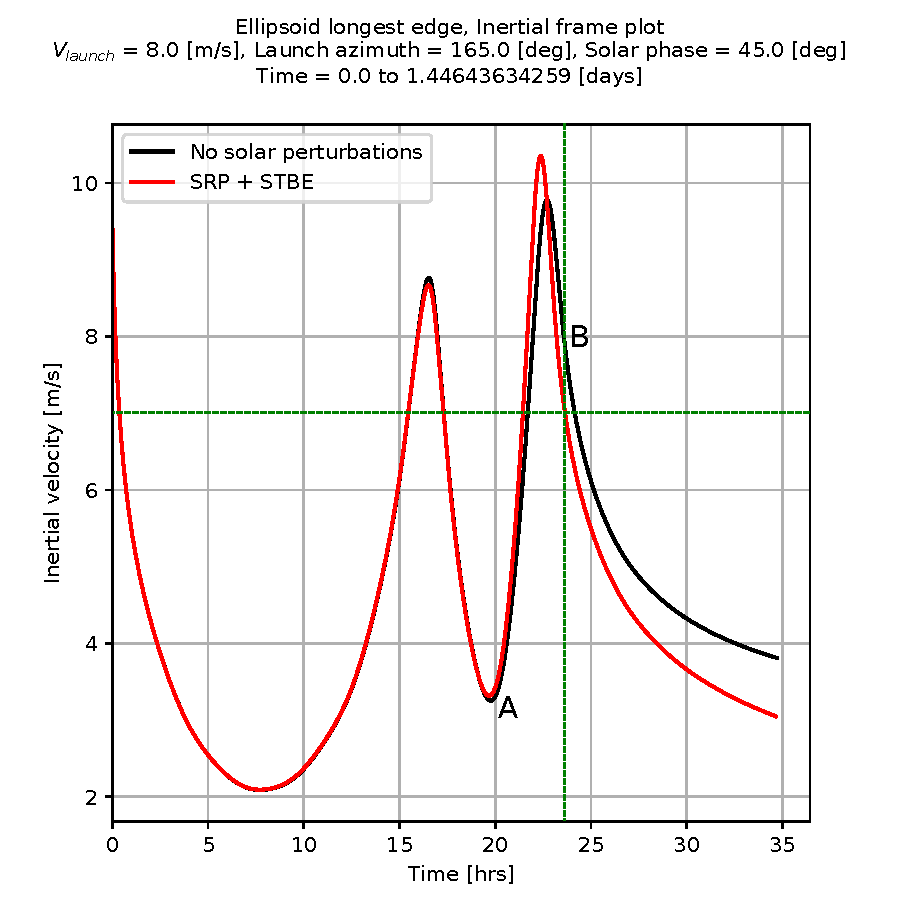
\includegraphics[width=\textwidth, height=0.5\textheight, keepaspectratio=true]{longest_edge_perturbations/3.2Density_1cmSize/8ms_165Azimuth_45SolarPhase/comparative_analysis_allPerturbations_inertialVelocity_edit.pdf}
\caption{Inertial velocity of the perturbed trajectory of capture case 8 in \Cref{tab:LoGSP_1_capture} compared with that of its unperturbed counterpart. The trajectories are shown for the time it takes for the particle in the unperturbed trajectory to escape. Particle code LoGSP-1.}
\label{fig:LoGSP_1_capture_case_8_comparative_inertial_velocity}
\end{figure}
\FloatBarrier
%%%
%%%
\begin{figure}[htb]
\centering
\captionsetup{justification=centering}
\subfloat[]{
    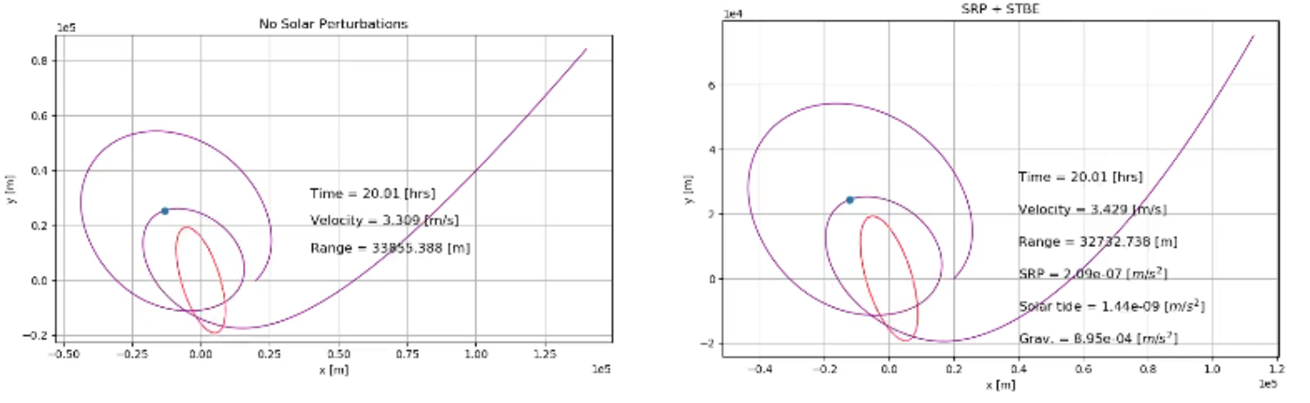
\includegraphics[angle=90, keepaspectratio]{longest_edge_perturbations/3.2Density_1cmSize/8ms_165Azimuth_45SolarPhase/comparative_analysis_animated_trajectory_snippet_initial_differences.pdf}
    \label{fig:LoGSP_1_capture_case_8_2d_comparative_animation_snippet}
}
\vline\vline
\subfloat[]{
    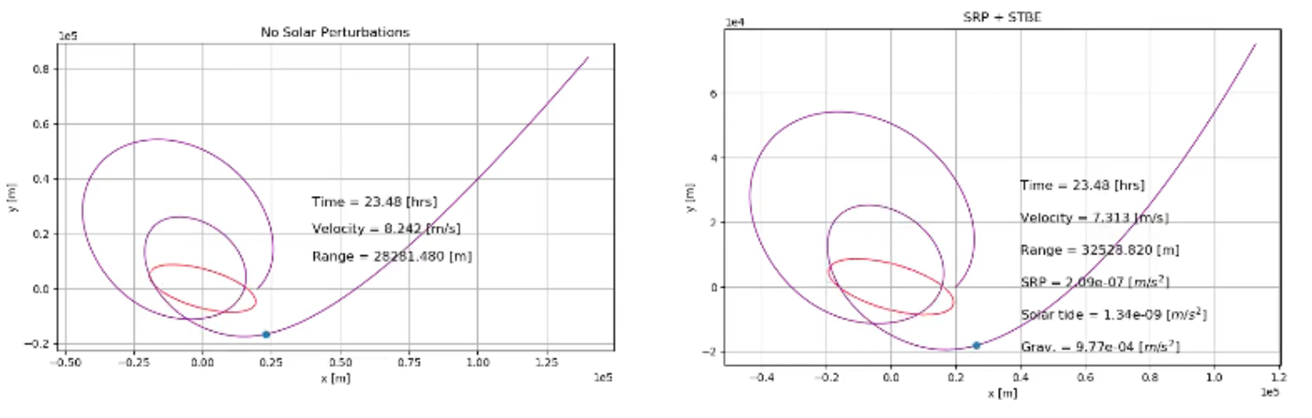
\includegraphics[angle=90, keepaspectratio]{longest_edge_perturbations/3.2Density_1cmSize/8ms_165Azimuth_45SolarPhase/comparative_analysis_animated_trajectory_snippet_escape_point.pdf}
    \label{fig:LoGSP_1_capture_case_8_2d_comparative_animation_phasingExample}
}
\caption{Animation snippets of the inertial frame 2D trajectory (XY-plane) of capture regolith for case number 8 in \Cref{tab:LoGSP_1_capture}. The bottom two plots are for the case when Solar perturbations were omitted from the simulation and the top two plots includes them. Note the differences in the range to the particle and its velocity for the same time stamp and rotational state of the asteroid. Particle code LoGSP-1.}
\label{fig:LoGSP_1_capture_case_8_comparative_animation_snapshots}
\end{figure}
\FloatBarrier
%%%
We see a similar effect when we look at capture case number 5 from \Cref{tab:LoGSP_1_capture}. The \gls{AIF} trajectory for it, both perturbed and unperturbed, are shown in \Cref{fig:LoGSP_1_capture_case_5_2d_trajectory_comparative_inertialFrame}. With Solar perturbations removed from the simulation, the initial conditions for this particle result in it getting launched on a highly elliptical orbit and eventually crashing onto the surface of the asteroid after 96 days. The particle, however, avoids this fate when Solar perturbations are included in the simulation. In \Cref{fig:LoGSP_1_capture_case_5_2d_trajectory_comparative_inertialFrame}, it can be clearly seen that the direction of the perturbing acceleration due to \gls{SRP} and \gls{STBE} is consistent with how the trajectory departs from its unperturbed counterpart. The trajectories are shown only for the time it takes for the particle in the unperturbed trajectory to re-impact the surface of the asteroid.
% We show this case to highlight the effect that perturbations have on a trajectory destined for re-impact, unlike the escape scenario discussed previously. We see drastic changes in the perturbed trajectory from the unperturbed one because when the particle is far away from the asteroid, the perturbing acceleration magnitude is of the same order as that of the gravitational acceleration.
% As a thought experiment, we see how the Solar phase angle at the time of launch is important in deciding the final fate of the regolith. We look at \Cref{fig:LoGSP_1_capture_case_5_2d_trajectory_comparative_srpEscape}, where the particle launch conditions are the same as that for the perturbed simulation in \Cref{fig:LoGSP_1_capture_case_5_2d_trajectory_comparative_inertialFrame} except that the initial Solar phase angle is 45.0 [deg] instead of 315.0 [deg]. The former results in an escape situation as the particle is just whisked away by the impeding \gls{SRP}.
%%%
\begin{figure}[htb]
\centering
\captionsetup{justification=centering}
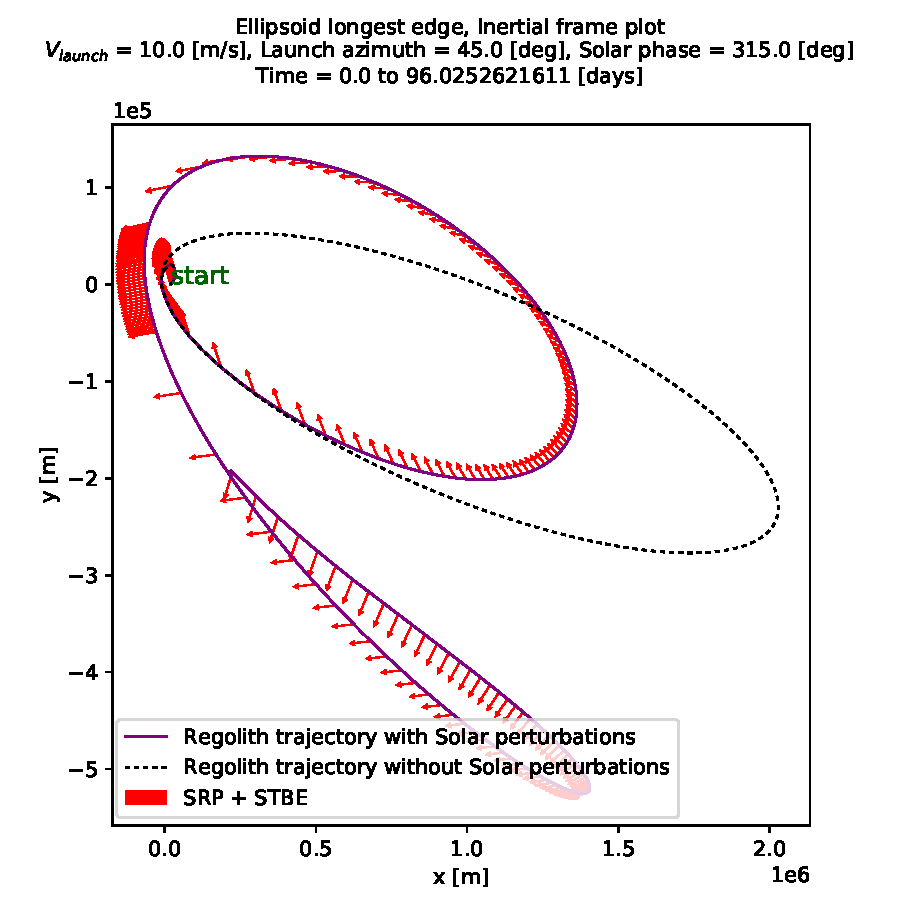
\includegraphics[width=\textwidth, height=0.5\textheight, keepaspectratio=true]{longest_edge_perturbations/3.2Density_1cmSize/singlePlot_comparative_PerturbationVector_10ms_45Azimuth_315SolarPhase_inertialFrame.pdf}
\caption{Inertial frame 2D trajectory (XY-plane) of capture regolith for case number 5 in \Cref{tab:LoGSP_1_capture} with direction of \gls{SRP} perturbation vector compared with the trajectory of a particle launched with the same initial conditions but in absence of Solar perturbations. Trajectories are shown for as long as it takes the unperturbed trajectory. Particle code LoGSP-1.}
\label{fig:LoGSP_1_capture_case_5_2d_trajectory_comparative_inertialFrame}
\end{figure}
\FloatBarrier
%%%
%%%
% \begin{figure}[htb]
% \centering
% \captionsetup{justification=centering}
% % another option for includegraphics - keepaspectratio
% 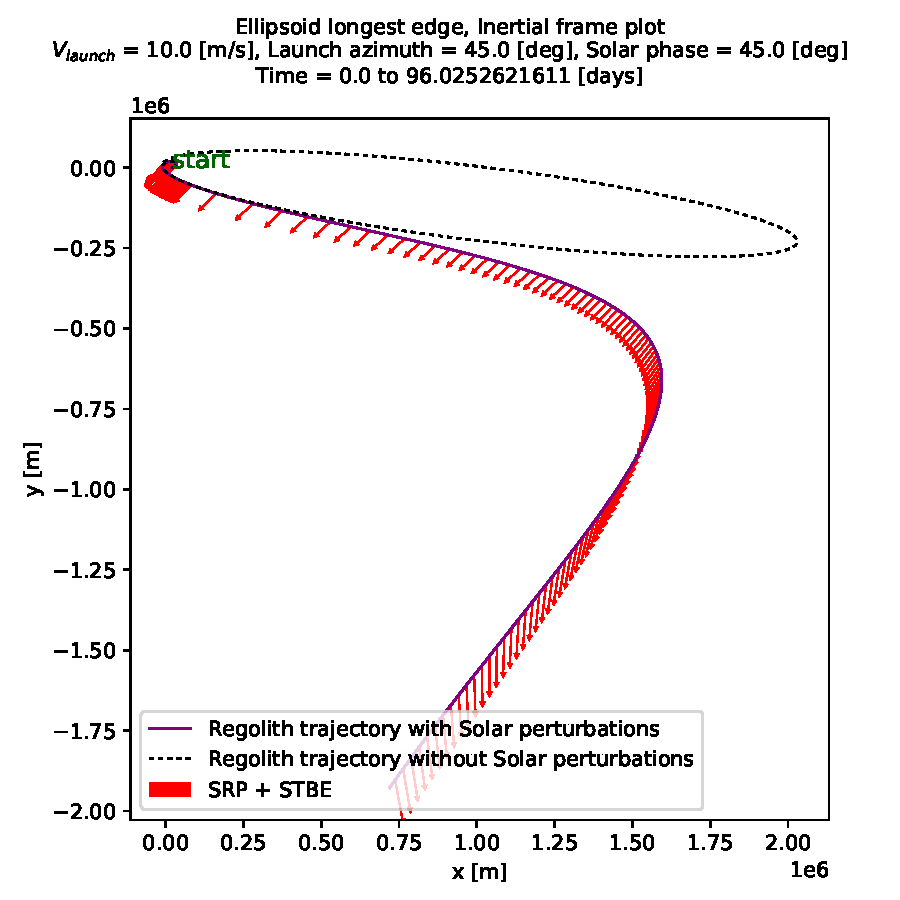
\includegraphics[width=\textwidth, height=0.5\textheight, keepaspectratio=true]{longest_edge_perturbations/3.2Density_1cmSize/srpEscape_comparative_10ms_45Azimuth_45SolarPhase_inertialFrame.pdf}
% \caption{Inertial frame 2D trajectory (XY-plane) of capture regolith for same launch velocity and launch azimuth as that of capture case number 5 in \Cref{tab:LoGSP_1_capture} but a different Solar phase angle of 45.0 [deg]. Particle code LoGSP-1.}
% \label{fig:LoGSP_1_capture_case_5_2d_trajectory_comparative_srpEscape}
% \end{figure}
% \FloatBarrier
%%%

\section{Final fate Behavior Of Different Regolith Types}
\label{sec:final_fate_general_all_launch_sites}
For simulations accounting Solar perturbations, the discussion so far has been about how perturbations affect particle motion and specifically the capture scenario, relative to a particle in an unperturbed simulation. We did this detailed analysis for a single particle type only, namely LoGSP-1 from \Cref{tab:area_to_mass_ratio}. We shall now look into the final fate behavior of all the regolith types mentioned in \Cref{tab:area_to_mass_ratio} to understand how particle motion is affected for different regolith densities and sizes. The simulations were conducted one-by-one for each regolith type, in the same manner as described earlier for particle LoGSP-1, but this time for three different launch sites.

\subsection{Regolith Loft From Longest Edge Of Asteroid}
\label{sec:general_char_longestEdge}
\Cref{fig:longestEdge_allParticles_reimpact_hist} shows the number of particles that resulted in re-impact after launch, for each particle type and initial Solar phase angle, against the launch velocity. Information about launch azimuth can not be derived from this plot. The overall trend\footnote{The trend over here is judged by looking at which grid cell the bars in the plot end up in.} remains the same across all plots for different initial Solar phases. There are small changes in the absolute numbers but they are significantly small and do not affect the qualitative property. From \Cref{fig:longestEdge_allParticles_reimpact_hist} we can infer that presence of Solar perturbations does not drastically affect the re-impact behavior of different regolith types.
%
\newline\newline
%
\Cref{fig:reimpact_traj_6ms_10Azim_multipleParticles_allSolarPhases} shows the xy-plane trajectories, an example that results in a re-impact scenario, for all regolith types mentioned in \Cref{tab:area_to_mass_ratio}. The particles have identical launch conditions for each initial Solar phase angle. What we witness from the plots is that for the same launch conditions that lead to a re-impact scenario, the trajectories remain almost similar and are not affected much by changes in regolith size and density. The similarity is also observed across different initial Solar phase angles. This implies that the perturbations are not significantly affecting the trajectories. We are looking at an isolated example here, but the fact that perturbations are not drastically affecting the re-impact trajectories is true to a very large extent and can be witnessed in the re-impact maps.
%
\newline\newline
%
Two re-impact maps are shown in \Cref{fig:longestEdge_crashmap_3.2_density_1cm_5cm_Radius,fig:longestEdge_crashmap_3.2_7.5_density_1cmRadius}. The former is for regoliths with the same density of \SI{3.2}{\gram\per\centi\metre\cubed} but particle radii 1 and \SI{5}{\centi\metre}; and the latter is for regoliths of the same particle radius of \SI{1}{\centi\metre} and densities 3.2 and \SI{7.5}{\gram\per\centi\metre\cubed}. What we see first-hand is that in the majority of cases, the re-impact locations for different regolith types are extremely similar. For the fewer cases where different particles have different re-impact locations, we see that the corresponding locations are very close to each other. This is also seen from the ending points on the trajectory plots in \Cref{fig:reimpact_traj_6ms_10Azim_45SolarPhase_multipleParticles,fig:reimpact_traj_6ms_10Azim_315SolarPhase_multipleParticles}. But from the majority, we can generalize that re-impact locations do not change significantly between different regolith types (used in this simulation and thesis) and/or with different initial Solar phase angles. Similar re-impact maps for regoliths with the density of \SI{7.5}{\gram\per\centi\metre\cubed} but particle radii 1 and \SI{5}{\centi\metre}; and for regoliths of the same particle radius of \SI{5}{\centi\metre} and densities 3.2 and \SI{7.5}{\gram\per\centi\metre\cubed}, are shown in \Cref{fig:longestEdge_crashmap_7.5_density_1cm_5cmRadius,fig:longestEdge_crashmap_3.2_7.5_density_5cmRadius} respectively.
% For even more rarer cases (wherein a common launch condition did not result in all particle types re-impacting), it was observed that the particles re-impacted at locations far away from each other.
%%%
\begin{figure}[htb]
\centering
\captionsetup{justification=centering}
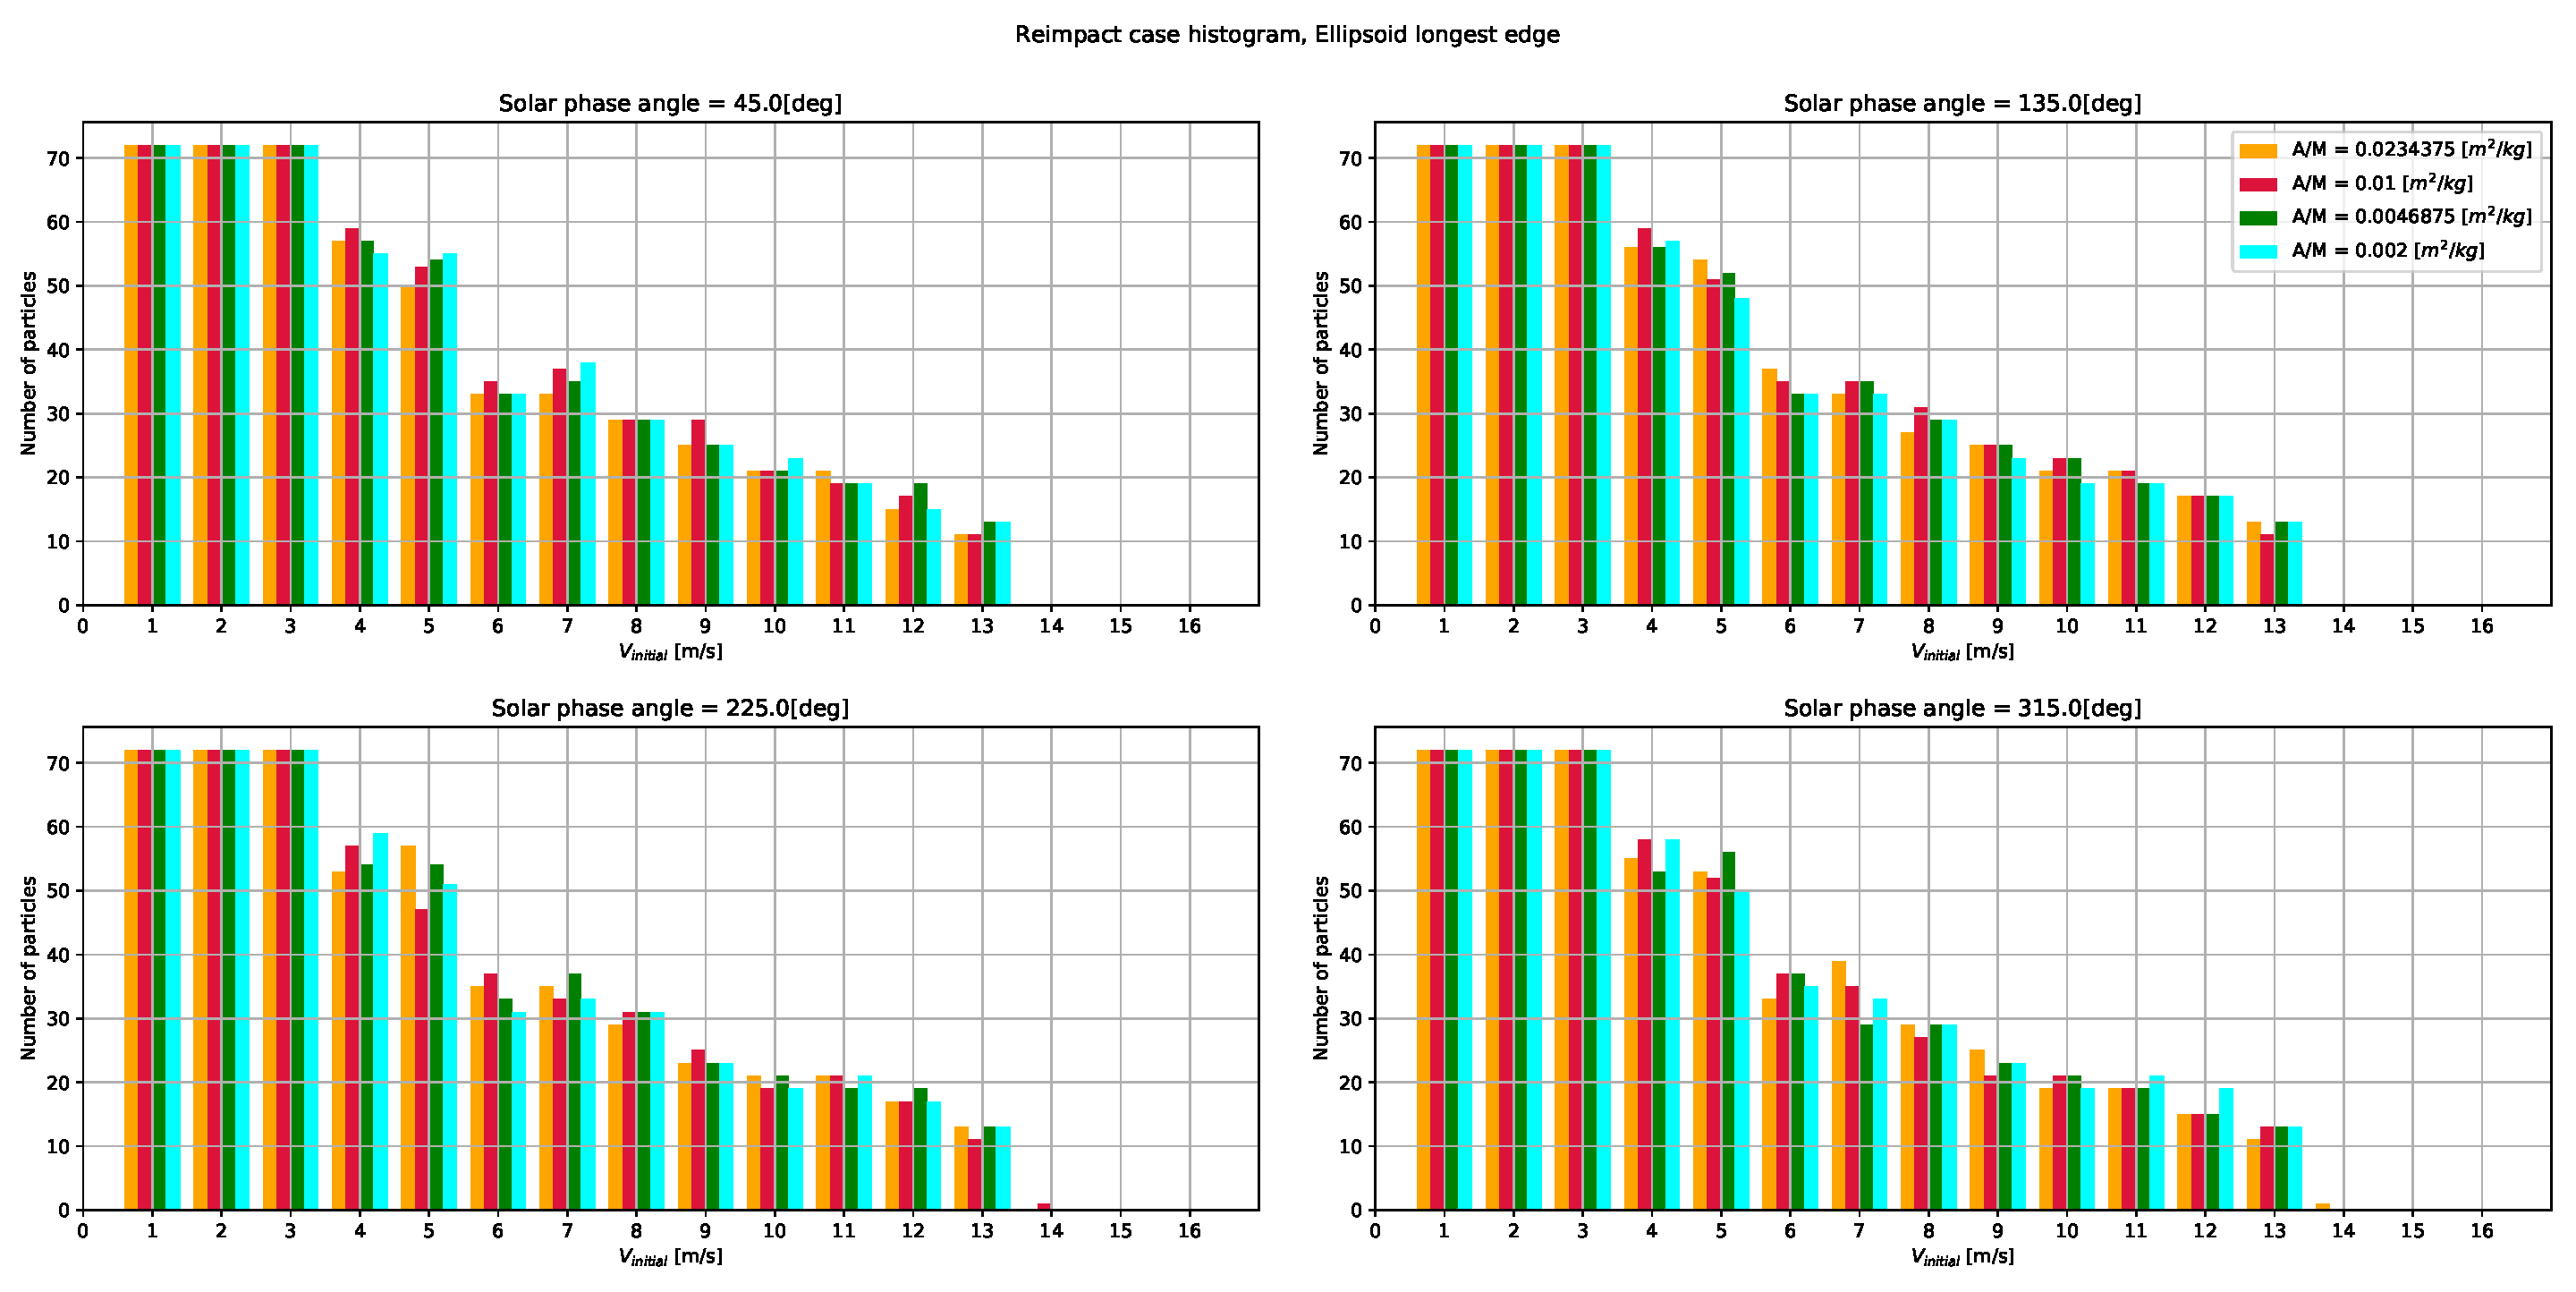
\includegraphics[angle=90, width=\textwidth, height=\textheight, keepaspectratio=true]{longest_edge_perturbations/multiple_regolith_types/allPhases_reimpactCases.pdf}
\caption{Number of re-impact cases for all regolith types launched from the longest edge of the asteroid. The densities and the particle size for the corresponding area-to-mass ratios can be found in \Cref{tab:area_to_mass_ratio}.}
\label{fig:longestEdge_allParticles_reimpact_hist}
\end{figure}
\FloatBarrier
%%%
%%%
\begin{figure}[htb]
\centering
\captionsetup{justification=centering}
\subfloat[]{
    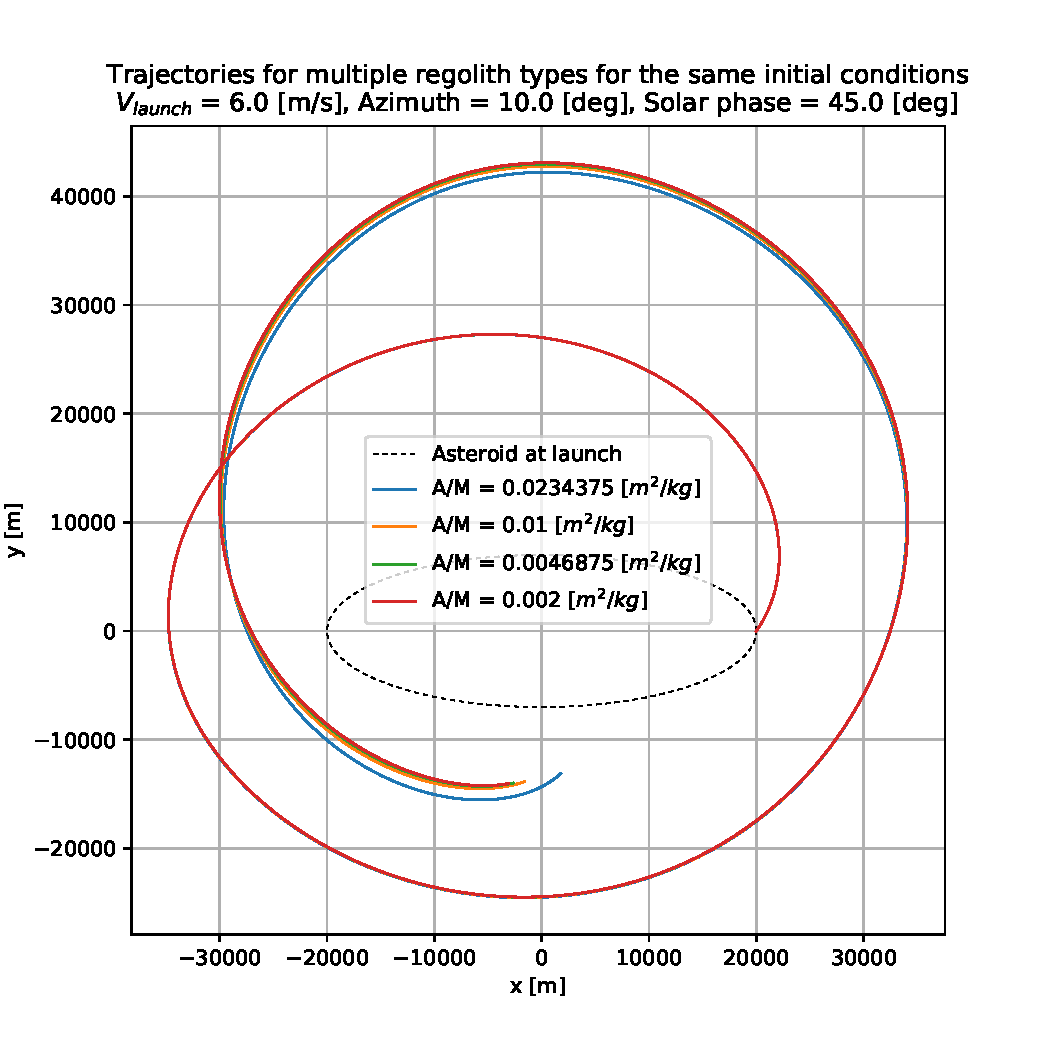
\includegraphics[width=0.5\textwidth, height=0.5\textheight, keepaspectratio=true]{longest_edge_perturbations/multiple_regolith_types/reimpact_traj_6ms_10Azim_45SolarPhase.pdf}
    \label{fig:reimpact_traj_6ms_10Azim_45SolarPhase_multipleParticles}
}
\subfloat[]{
    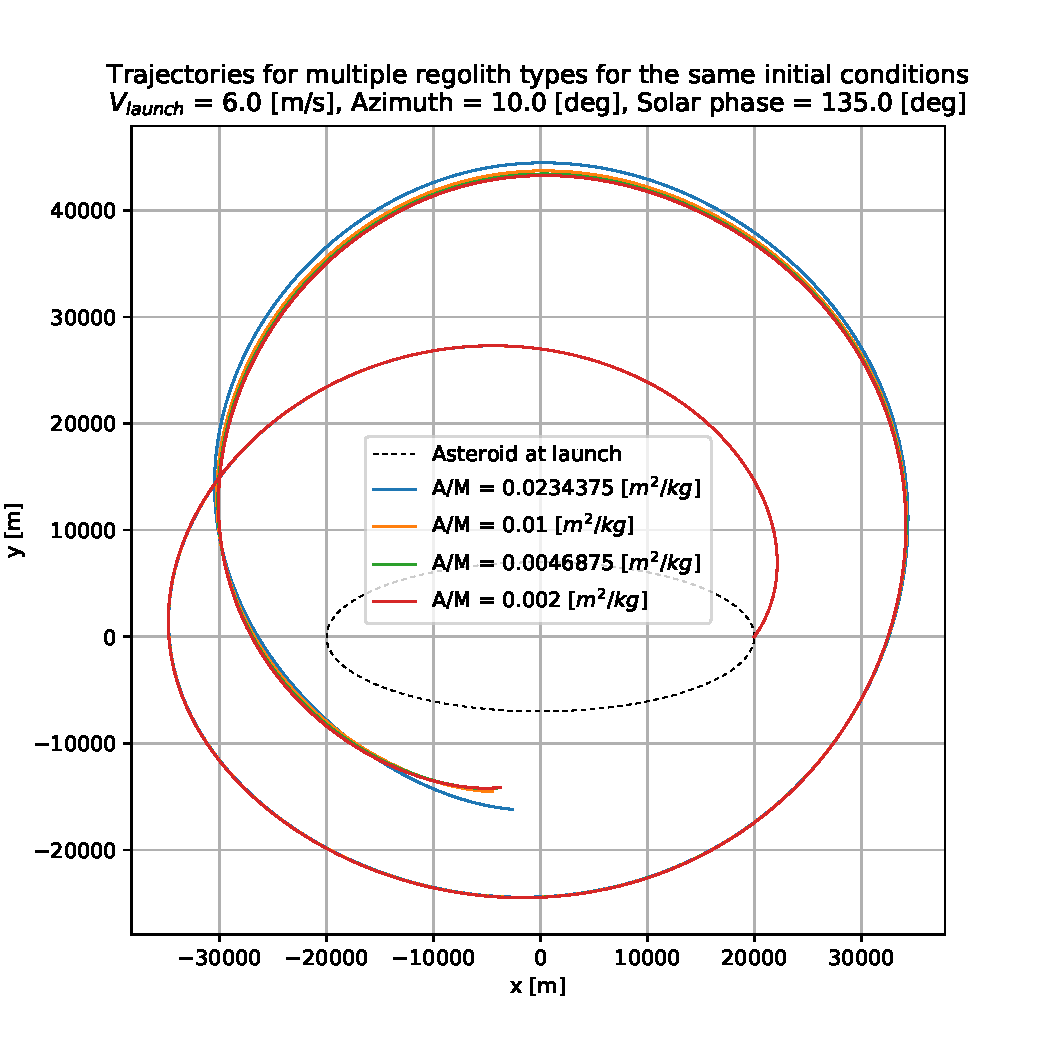
\includegraphics[width=0.5\textwidth, height=0.5\textheight, keepaspectratio=true]{longest_edge_perturbations/multiple_regolith_types/reimpact_traj_6ms_10Azim_135SolarPhase.pdf}
    \label{fig:reimpact_traj_6ms_10Azim_135SolarPhase_multipleParticles}
}

\subfloat[]{
    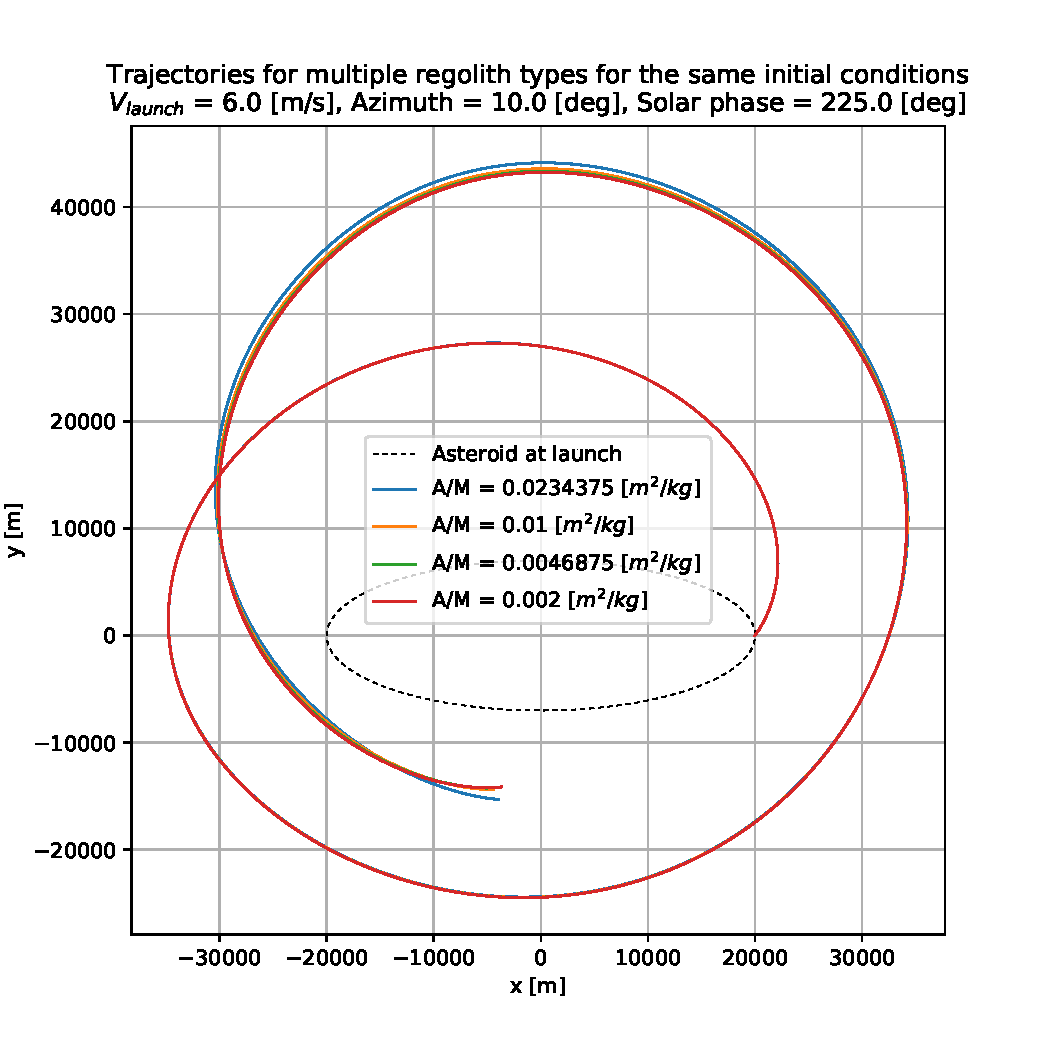
\includegraphics[width=0.5\textwidth, height=0.5\textheight, keepaspectratio=true]{longest_edge_perturbations/multiple_regolith_types/reimpact_traj_6ms_10Azim_225SolarPhase.pdf}
    \label{fig:reimpact_traj_6ms_10Azim_225SolarPhase_multipleParticles}
}
\subfloat[]{
    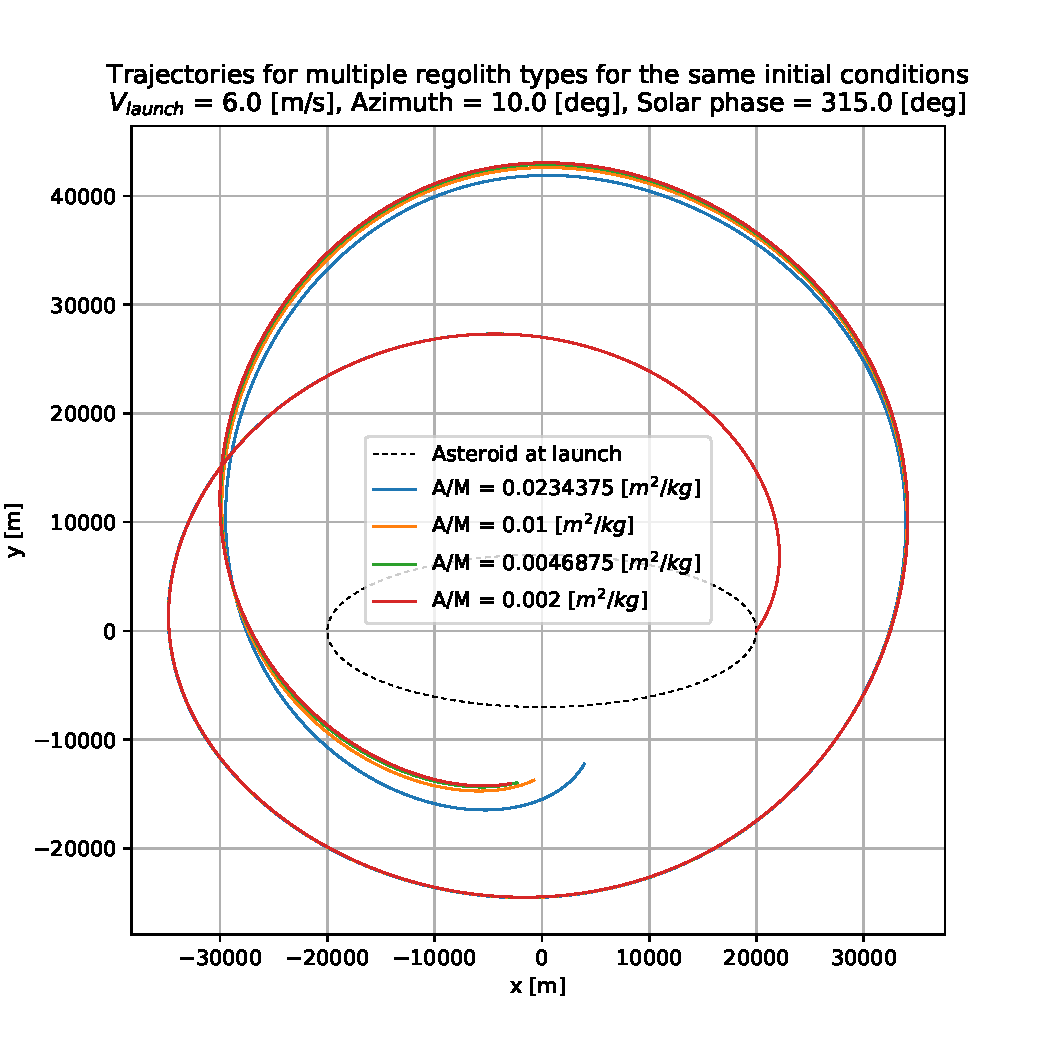
\includegraphics[width=0.5\textwidth, height=0.5\textheight, keepaspectratio=true]{longest_edge_perturbations/multiple_regolith_types/reimpact_traj_6ms_10Azim_315SolarPhase.pdf}
    \label{fig:reimpact_traj_6ms_10Azim_315SolarPhase_multipleParticles}
}
\caption{Re-impact trajectories for all regolith types mentioned in \Cref{tab:area_to_mass_ratio}. The trajectories are shown for different initial Solar phase values but for each, the launch conditions are identical for all particle types. The trajectories are expressed in the \gls{AIF} and the point where the trajectories abruptly end is where the re-impact occurs with the rotating asteroid.}
\label{fig:reimpact_traj_6ms_10Azim_multipleParticles_allSolarPhases}
\end{figure}
\FloatBarrier
%%%
%%%
\begin{figure}[htb]
\centering
\captionsetup{justification=centering}
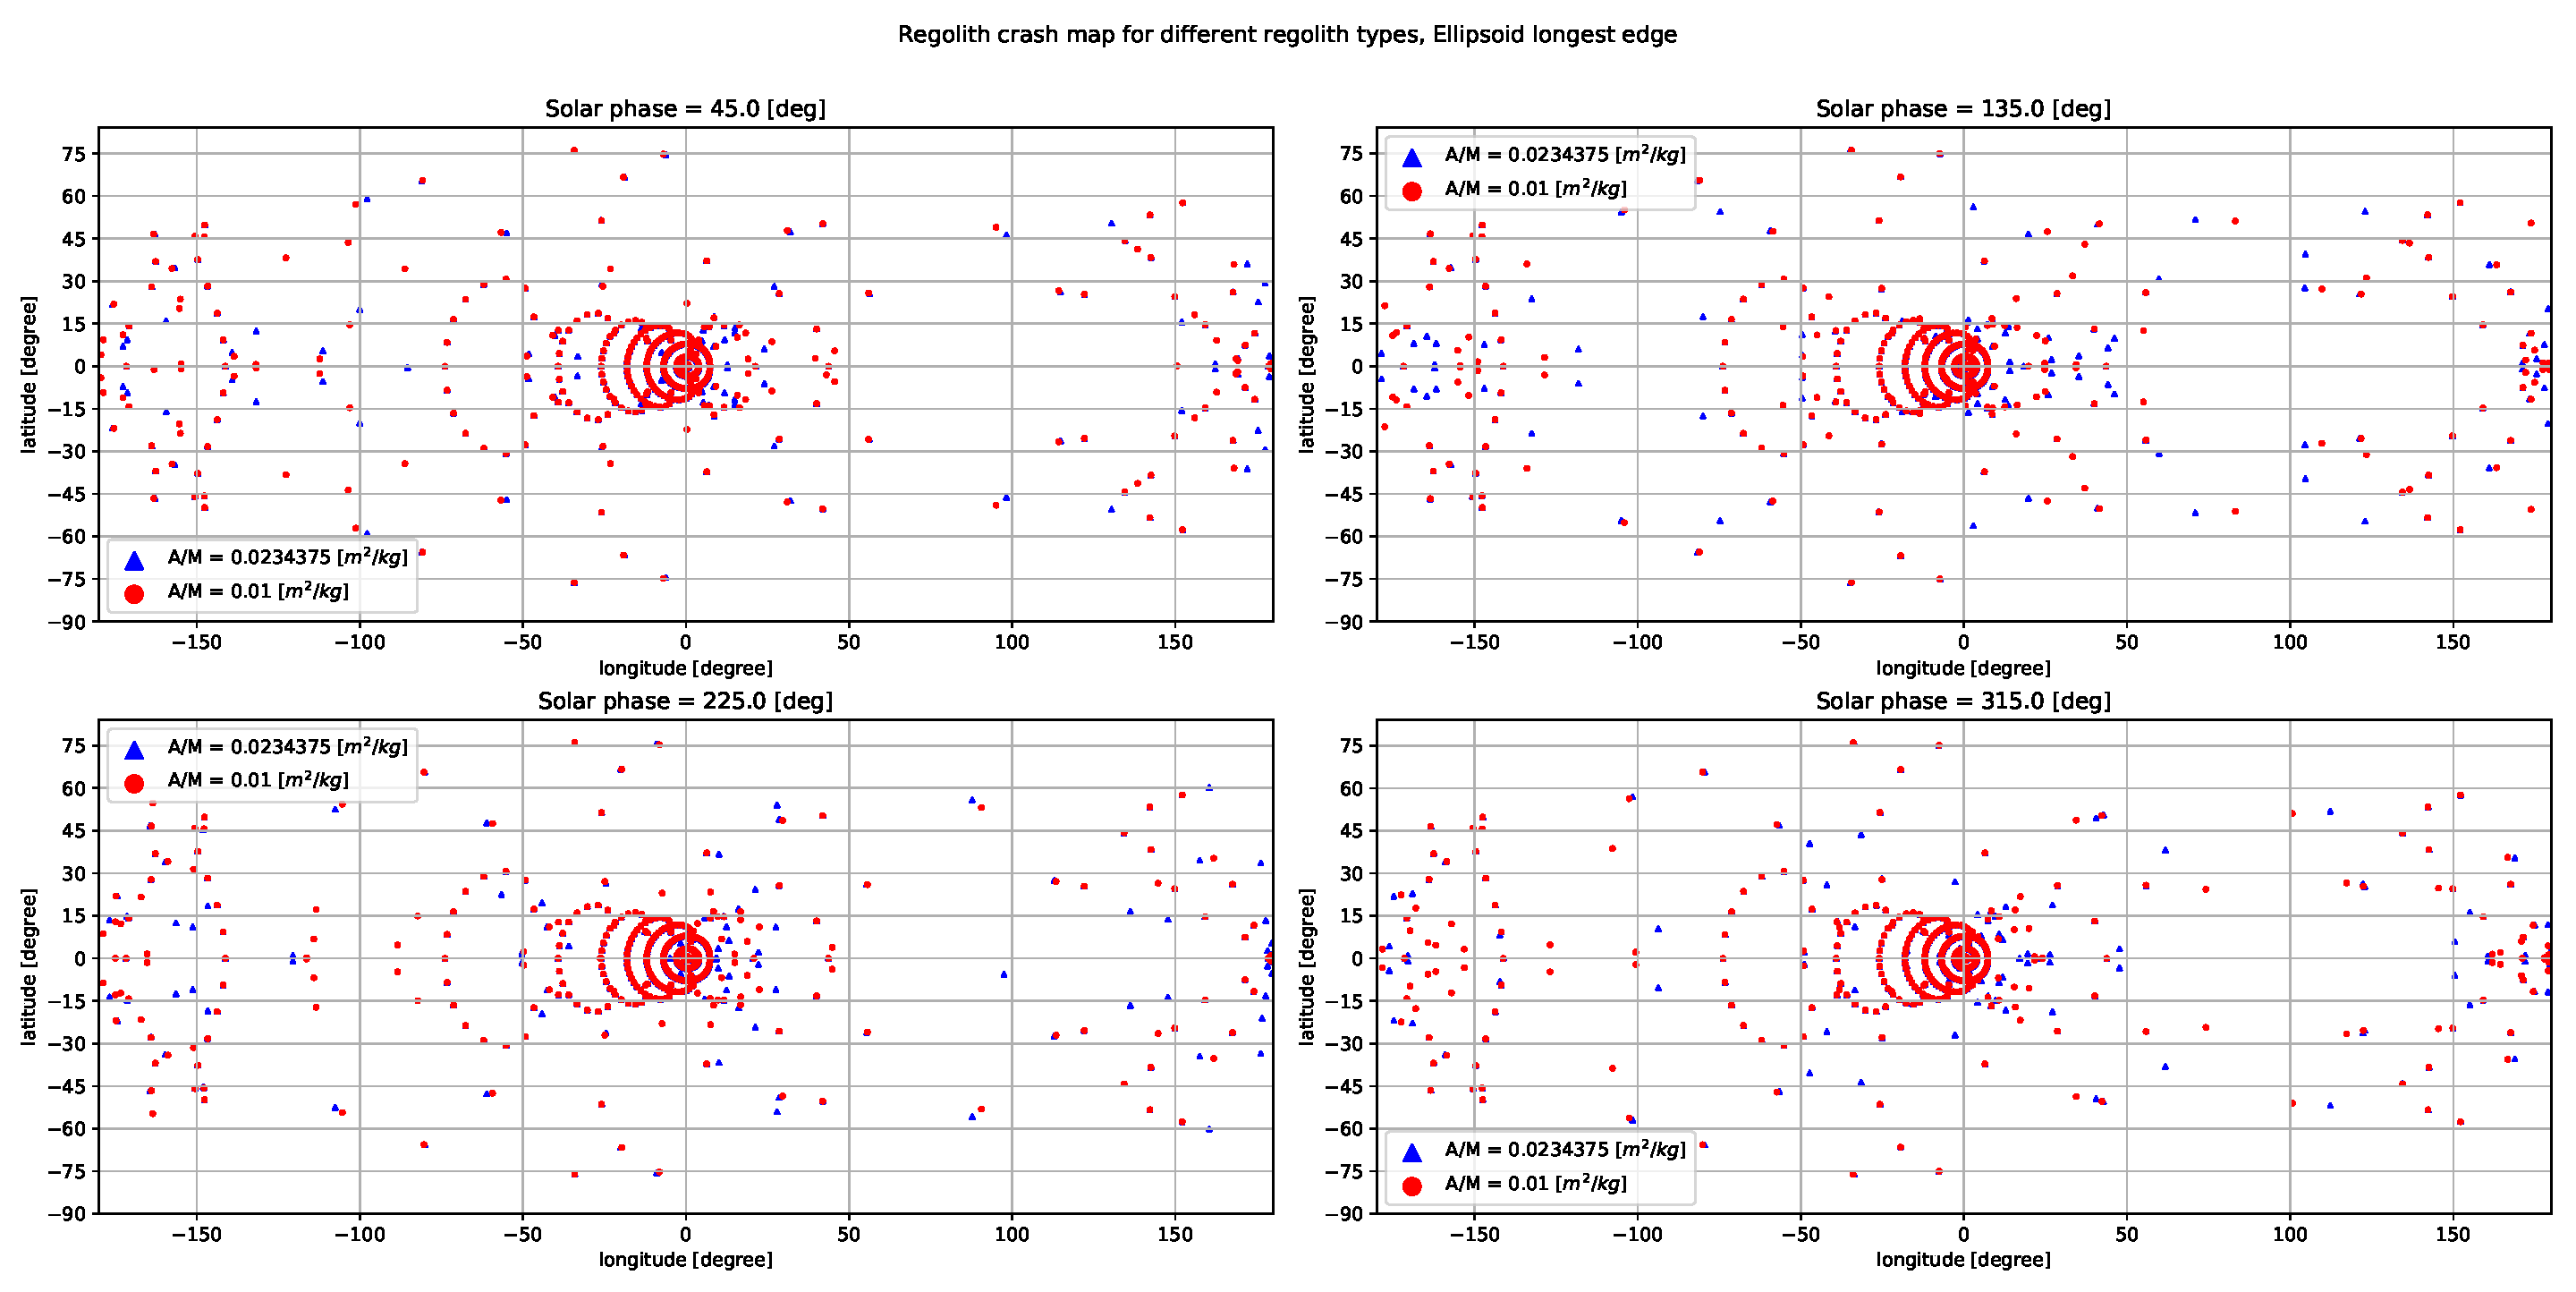
\includegraphics[angle=90, width=\textwidth, height=\textheight, keepaspectratio=true]{Results/Images/longest_edge_perturbations/multiple_regolith_types/allPhases_crashMap_3P2_7P5_density_1cm_Radius.pdf}
\caption{Re-impact locations for regoliths of different density but same size (i.e 1 cm). The densities and the particle size for the corresponding area-to-mass ratios can be found in \Cref{tab:area_to_mass_ratio}.}
\label{fig:longestEdge_crashmap_3.2_7.5_density_1cmRadius}
\end{figure}
\FloatBarrier
%%%
\Cref{fig:longestEdge_allParticles_escape_hist} shows the number of cases that lead to an escape situation for all regolith types and for different initial Solar phase angles. Just like that for the re-impact case, what we observe here is that the general trend of the number of cases does not vary much with different initial Solar phase angles. Although, fluctuations in exact numbers are visible. For extremely high velocities, \SI{15}{\metre\per\second} and beyond, the particles always escape and are not affected by the presence of the Solar perturbations.
%
\newline\newline
%
\Cref{fig:longestEdge_allParticles_escape_hev_solarPhase45} shows the variation in the \gls{HEV} with launch azimuth, for three different launch velocities and for an initial Solar phase angle of \SI{45}{\degree}. For the remaining Solar phases, the plots are similar and can be found in the appendix in \Cref{fig:longestEdge_allParticles_escape_hev_solarPhase135,fig:longestEdge_allParticles_escape_hev_solarPhase225,fig:longestEdge_allParticles_escape_hev_solarPhase315}. In the plot for velocity \SI{13}{\metre\per\second} we see that the escape behavior is identical for all particle types as the data points for each overlap one another. As previously discussed, for uniform and smooth distribution of \gls{HEV} data points, the particles are on an escape trajectory immediately after launch and do not require an assist from the rapid rotation of the asteroid. The latter is required, for example, in the case of \SI{5}{\metre\per\second} as observed from the uneven distribution of the \gls{HEV} data points. Thus for smaller velocities, the \gls{HEV} data points for different regolith types are not overlapping, suggesting that the perturbations have a significant effect on their trajectories. But as the velocities increase, the perturbations have lesser of an effect on the trajectories. Another way of saying this is that when the launch velocity is itself large, the particles are on a relatively quicker escape trajectory, which means that the perturbing acceleration does not surmount to a value that can cause significant changes. This is also observed in the trajectory plots for all the particles.
%
\newline\newline
%
\Cref{fig:escape_traj_allParticles_5ms_225Azim_45solarPhase} shows the trajectories for a launch velocity of \SI{5}{\metre\per\second}, launch azimuth of \SI{225}{\degree} and an initial Solar phase angle of \SI{45}{\degree}. \Cref{fig:escape_traj_allParticles_9ms_225Azim_45solarPhase} shows the trajectory for a launch velocity of \SI{9}{\metre\per\second} with all other initial conditions being the same. We see that for a higher velocity, all regolith types have the same escape behavior or trajectory and are hardly affected by the Solar perturbations. For the smaller velocity, we see that all particles are distinctly separated as they embark on the escape trajectory in the end. The difference is significantly large. A zoomed-in version of the trajectory plot for the case of \SI{5}{\metre\per\second} is shown in \Cref{fig:escape_traj_allParticles_5ms_225Azim_45solarPhase_zoomed}. For the example case depicted in \Cref{fig:escape_traj_allParticles_5ms_225Azim_45solarPhase}, and keeping in mind that the initial Solar phase angle is \SI{45}{\degree}, the differences in the trajectories start emerging slowly much earlier in the simulation (even before the first revolution is completed), with the highest area-to-mass ratio particle getting pushed outwards (due to a higher \gls{SRP} effect) relative to the one with the lowest area-to-mass ratio. As explained previously for the capture scenario, in this case too, we witness that different regolith types are subject to different phasing with respect to the asteroid. Thus as the particles approach the vicinity of the asteroid, the existing trajectory differences (or phase differences) get amplified by the rapid rotation of the asteroid, leading to four distinct escape routes.
%
\newline\newline
%
\Cref{fig:longestEdge_allParticles_capture_hist} shows the number of capture cases for all regolith types. The number of capture cases is extremely small relative to the number of escape and re-impact cases shown previously. We will look at the trajectory of an example capture case from \Cref{fig:longestEdge_allParticles_capture_hist}, i.e. particle LoGSP-4, at launch velocity \SI{6}{\metre\per\second}, launch azimuth of \SI{20}{\degree}, and initial Solar phase angle of \SI{45}{\degree}. For the same launch conditions, the trajectories for the remaining regolith types were also plotted, neither of which resulted in capture, and are shown in \Cref{fig:allRegolith_traj_6ms_20Azim_45solarPhase}. The reasons for separation of the trajectories for the different regolith types, in this situation, is the same as explained recently for the escape scenario. Due to Solar perturbations, the trajectory for each particle is shifted such that each has a different phase with respect to the rotating asteroid. The only difference here, is that all particles do not share the same fate as each other.
% A zoomed in version of the trajectory, highlighting the visible separation in the regolith trajectories is shown in \Cref{fig:allRegolith_traj_6ms_20Azim_45solarPhase_zoomed}.
%%%
\begin{figure}[htb]
\centering
\captionsetup{justification=centering}
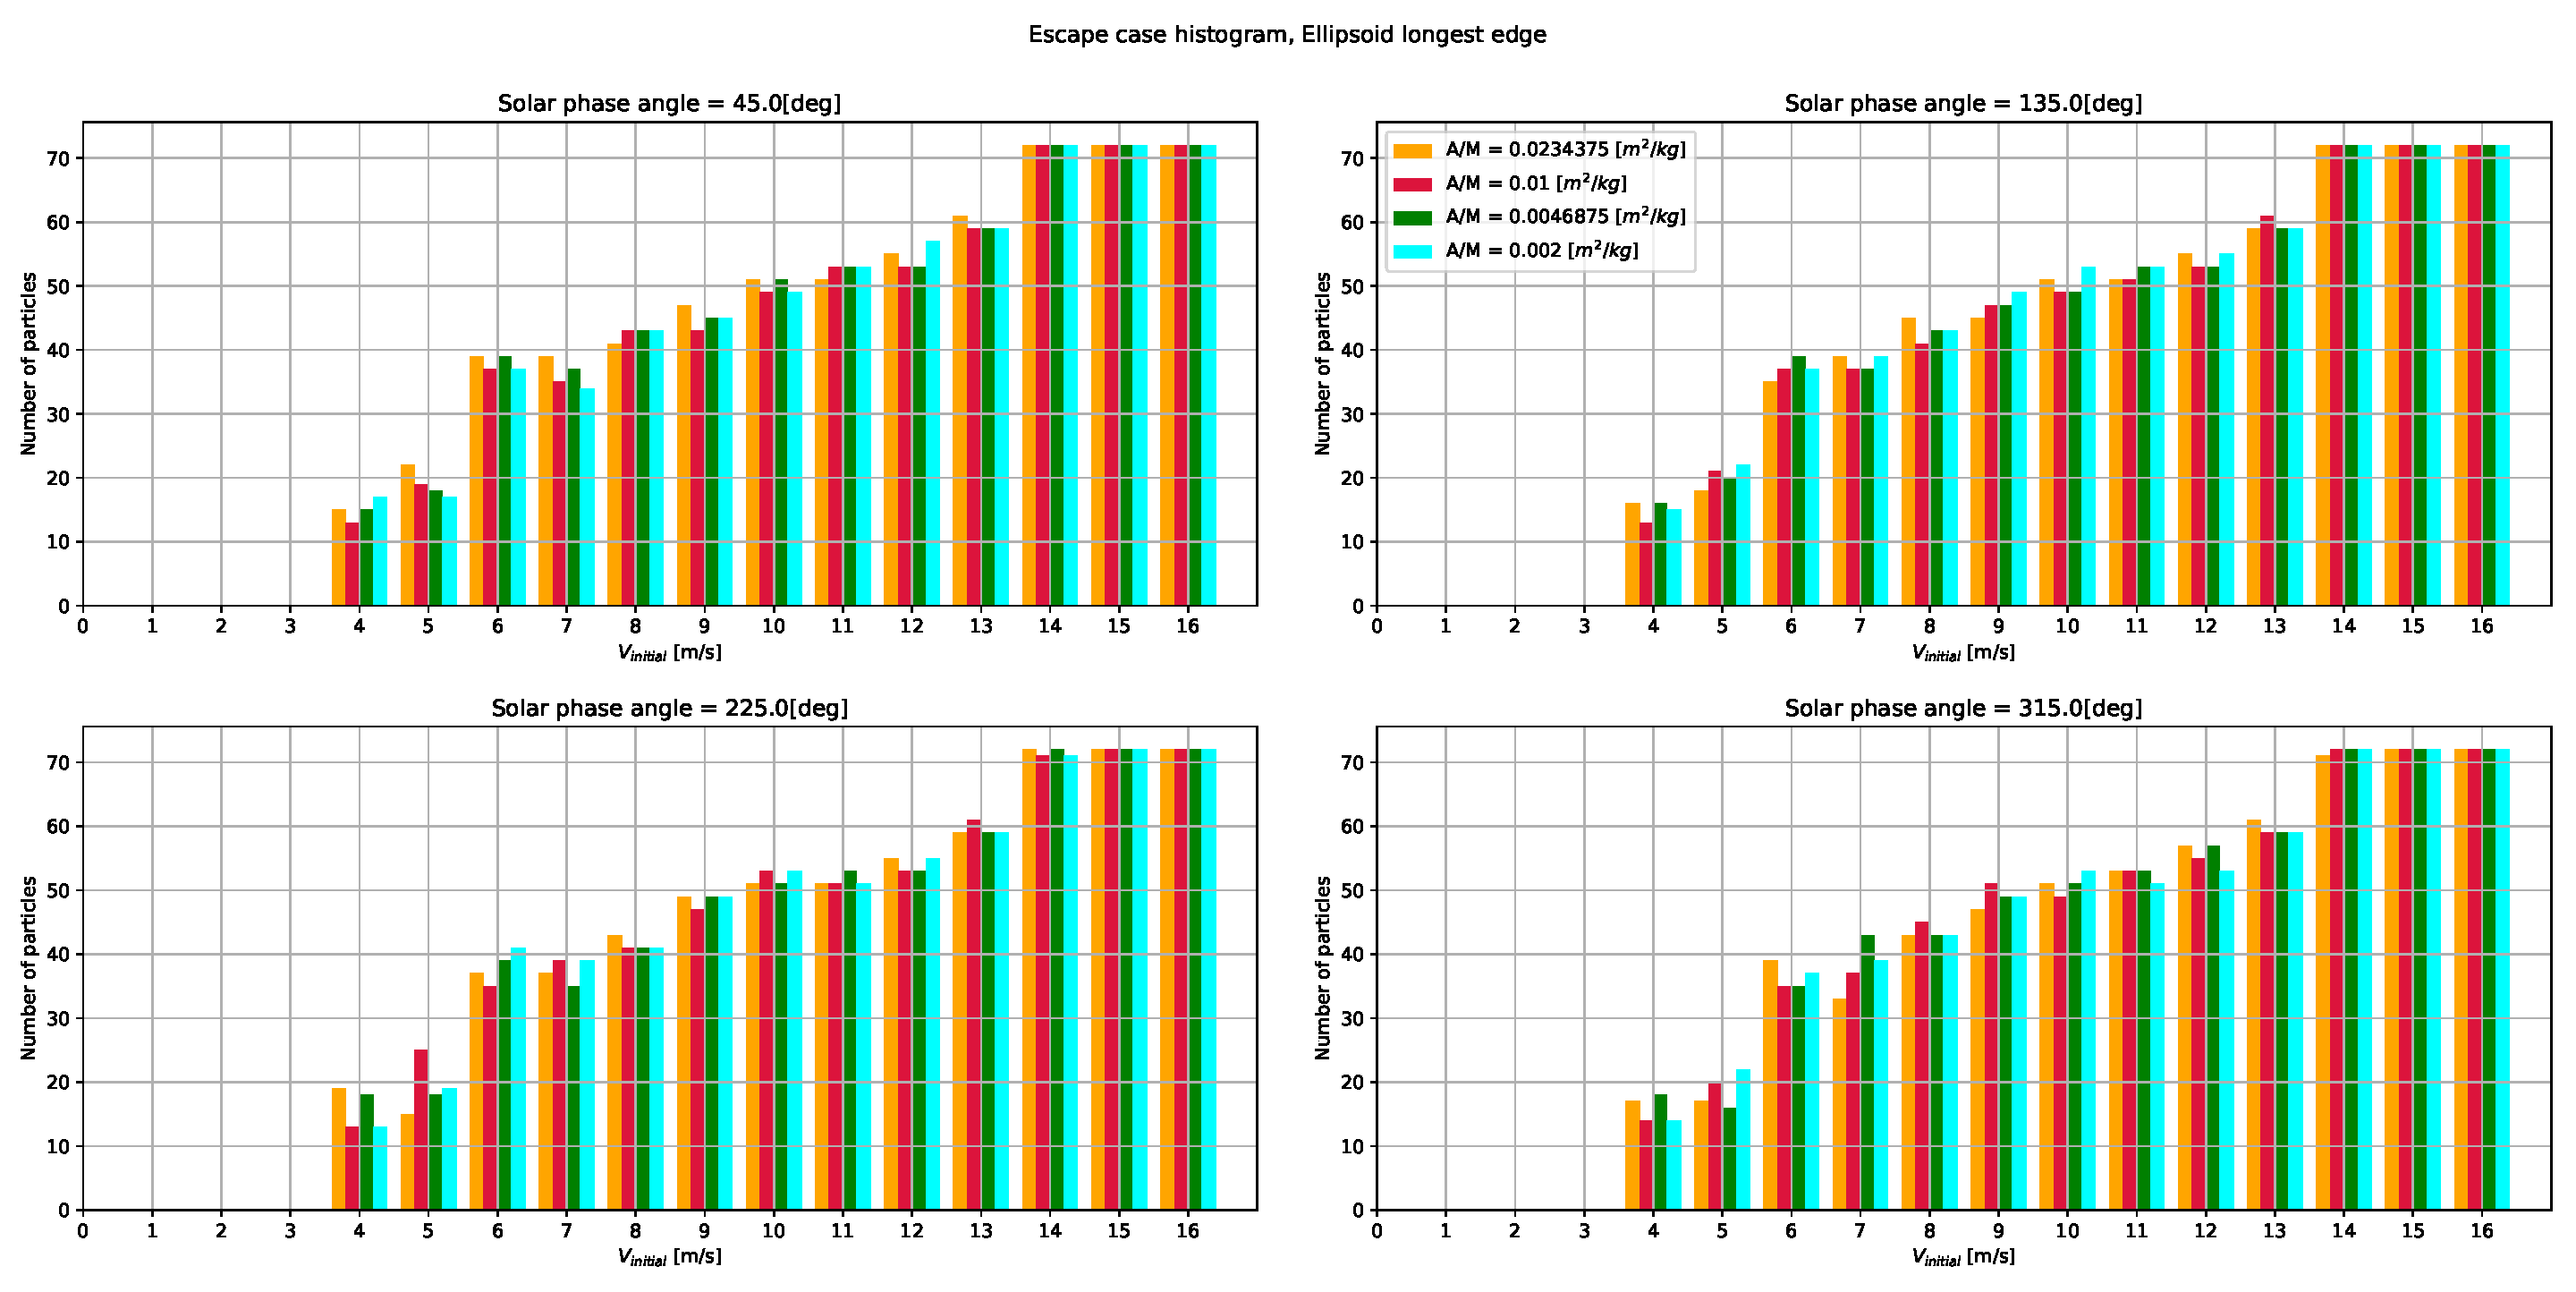
\includegraphics[angle=90, width=\textwidth, height=\textheight, keepaspectratio=true]{longest_edge_perturbations/multiple_regolith_types/allPhases_escapeCases.pdf}
\caption{Number of all escape cases for all regolith types launched from the longest edge of the asteroid. The densities and the particle size for the corresponding area-to-mass ratios can be found in \Cref{tab:area_to_mass_ratio}.}
\label{fig:longestEdge_allParticles_escape_hist}
\end{figure}
\FloatBarrier
%%%
%%%
\begin{figure}[htb]
\centering
\captionsetup{justification=centering}
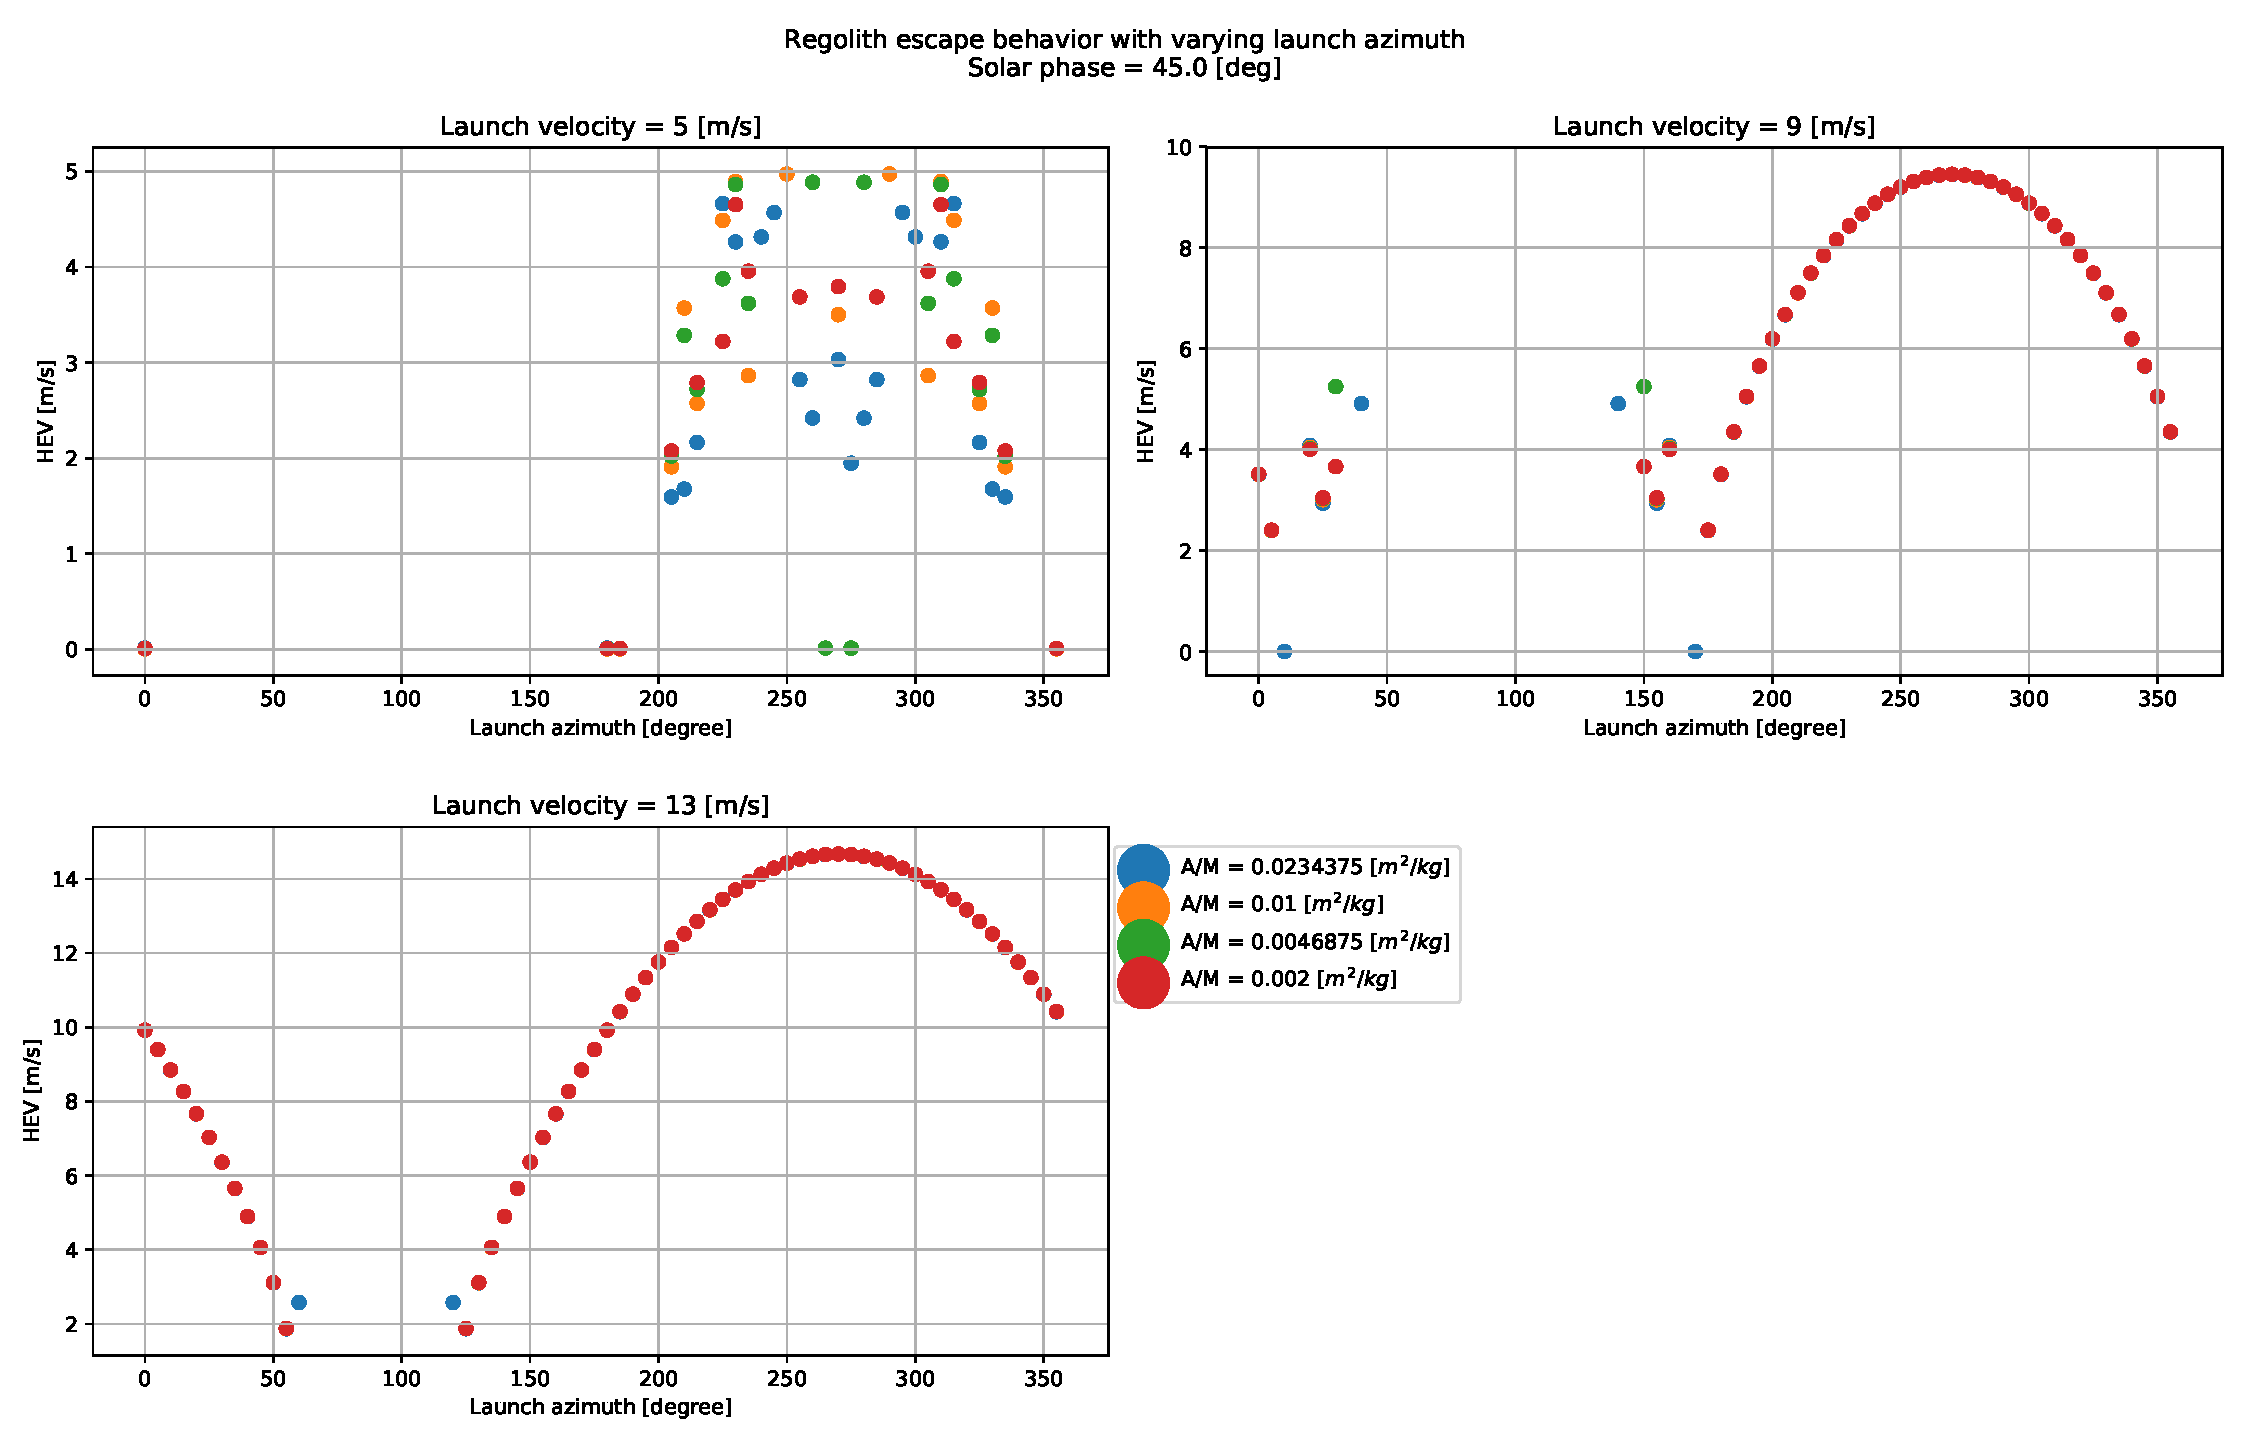
\includegraphics[width=\textwidth, height=0.5\textheight, keepaspectratio=true]{longest_edge_perturbations/multiple_regolith_types/phase45_escapeHEV.pdf}
\caption{\gls{HEV}, shown for all regolith types used in this thesis, but only for three specific launch velocities. The densities and the particle size for the corresponding area-to-mass ratios can be found in \Cref{tab:area_to_mass_ratio}.}
\label{fig:longestEdge_allParticles_escape_hev_solarPhase45}
\end{figure}
\FloatBarrier
%%%
%%%
\begin{figure}[!h]
\centering
\captionsetup{justification=centering}
\subfloat[]{
    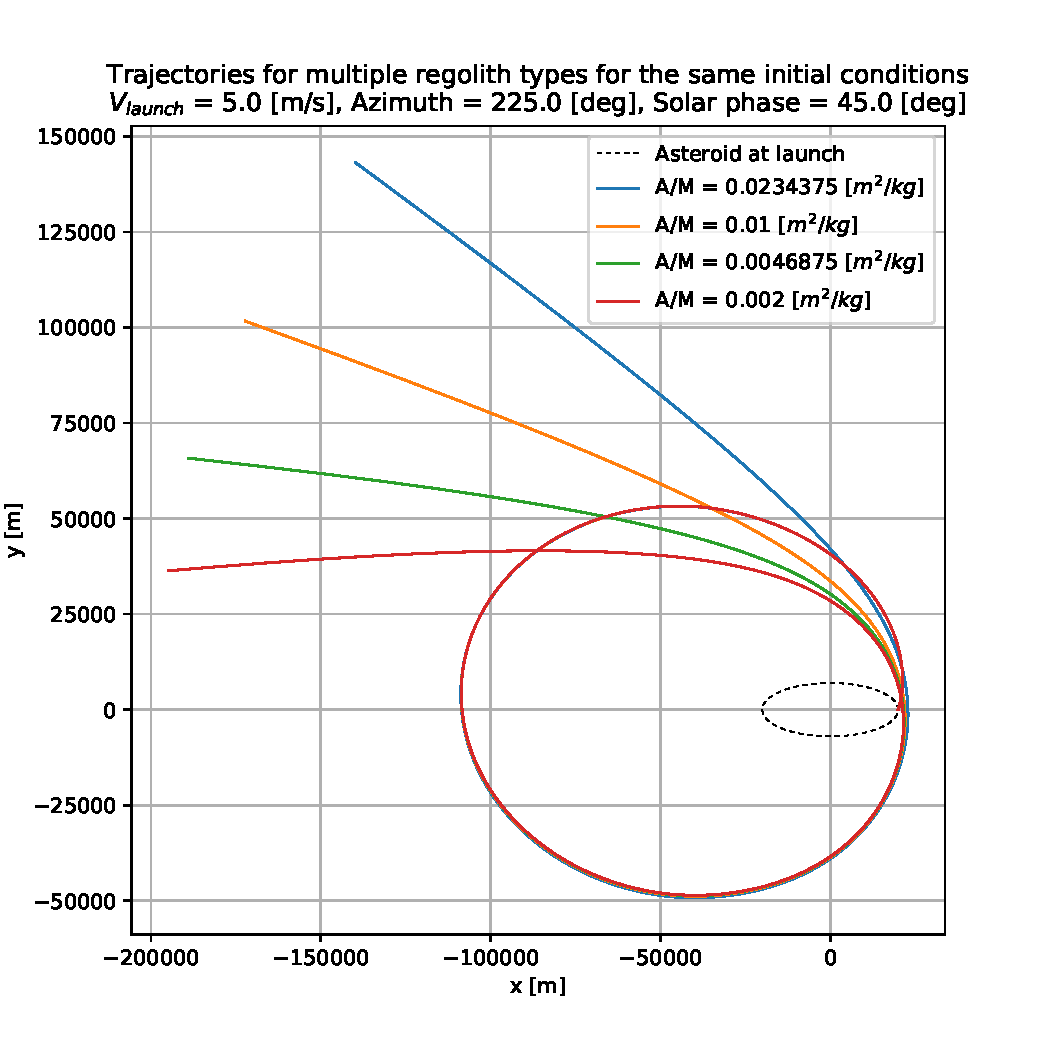
\includegraphics[width=0.5\textwidth, height=0.5\textheight, keepaspectratio=true]{longest_edge_perturbations/multiple_regolith_types/escape_traj_5ms_225Azim_45solarPhase.pdf}
    \label{fig:escape_traj_allParticles_5ms_225Azim_45solarPhase}
}
\subfloat[]{
    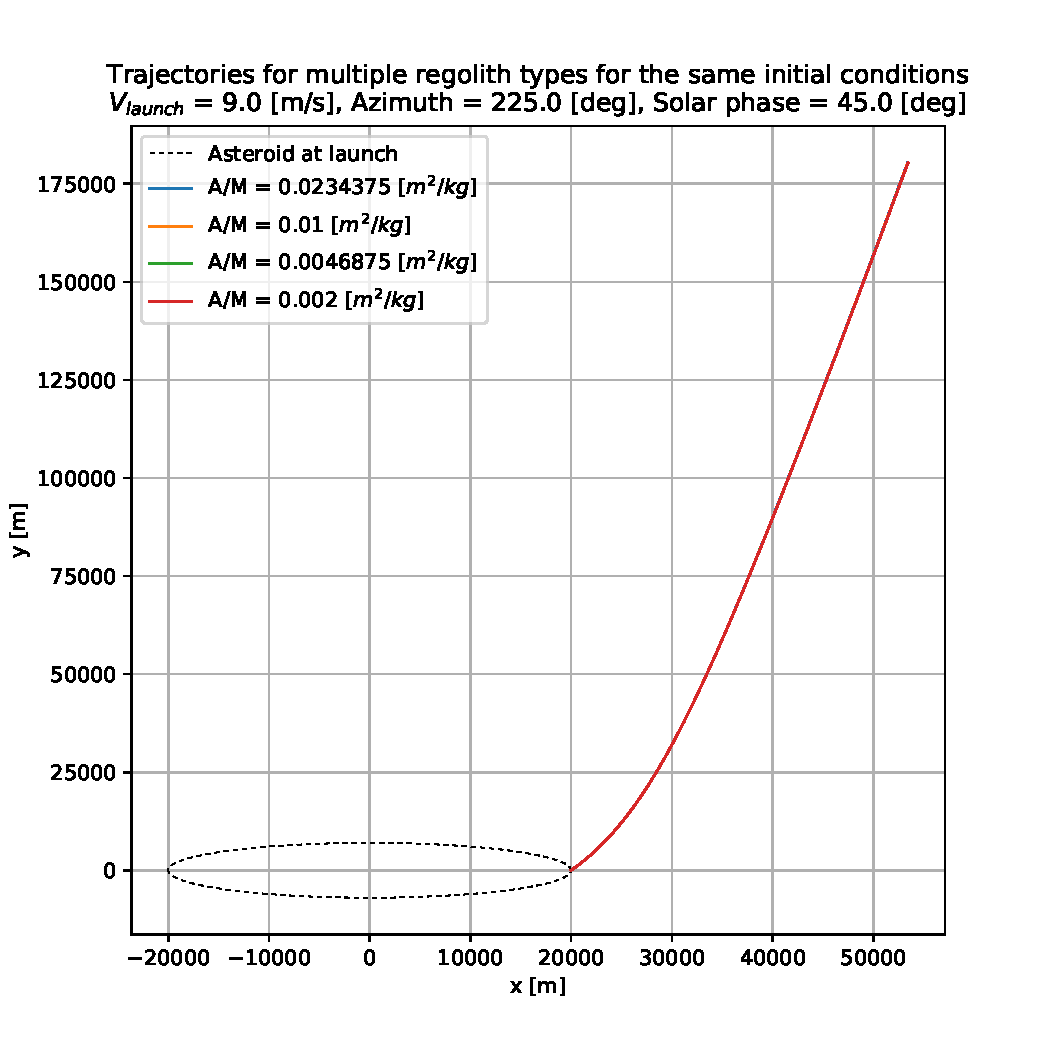
\includegraphics[width=0.5\textwidth, height=0.5\textheight, keepaspectratio=true]{longest_edge_perturbations/multiple_regolith_types/escape_traj_9ms_225Azim_45solarPhase.pdf}
    \label{fig:escape_traj_allParticles_9ms_225Azim_45solarPhase}
}
\caption{Escape trajectories for all regolith types, highlighting the diminishing effect of Solar perturbations as the launch velocity increases (keeping all other initial conditions same). The densities and the particle size for the corresponding area-to-mass ratios can be found in \Cref{tab:area_to_mass_ratio}.}
\label{fig:escape_traj_allParticles_5ms_9ms_225Azim_45solarPhase}
\end{figure}
\FloatBarrier
%%%
%%%
\begin{figure}[htb]
\centering
\captionsetup{justification=centering}
\includegraphics[width=\textwidth, height=0.5\textheight, keepaspectratio=true]{longest_edge_perturbations/multiple_regolith_types/allPhases_captureCases.pdf}
\caption{Number of all capture cases for all regolith types launched from the longest edge of the asteroid. The densities and the particle size for the corresponding area-to-mass ratios can be found in \Cref{tab:area_to_mass_ratio}.}
\label{fig:longestEdge_allParticles_capture_hist}
\end{figure}
\FloatBarrier
%%%
\subsection{Regolith Loft From Leading Edge Of Asteroid}
\label{sec:general_char_leadingEdge}
\Cref{fig:leadingEdge_allParticles_reimpact_hist} shows the total number of re-impact cases for all regolith types launched from a fixed location on the leading edge of the asteroid. The number of re-impact cases are far more than those observed for the longest edge scenario. Even for a relatively high velocity of \SI{11}{\metre\per\second}, all particles result in a re-impact. Their are two reasons for this behavior. The first is that the gravitational attraction for the current launch location is stronger than that on the longest edge of the asteroid. The latter has the weakest gravitational attraction on the entire ellipsoid shaped asteroid. The second is that the particles have a much lower inertial velocity at rest (due to the asteroid's rotation) at the current launch site as it is radially closer (from the centre of the asteroid) to the axis of rotation, compared to that for a launch site at the longest edge of the asteroid. Thus, we see an increase in the number of re-impact cases and especially for the higher velocities.
%
\newline\newline
%
The presence of Solar radiation pressure has no significant effect on the particle trajectories. Compared to the longest edge, there are fewer cases where different regolith types have distinct re-impact locations. We observe this in the re-impact maps shown in \Cref{fig:crashmap_3.2_7.5_density_1cmRadius_leadingEdge}, where regoliths have the same particle radii of \SI{1}{\centi\metre} and densities 3.2 and \SI{7.5}{\gram\per\centi\metre\cubed}; and \Cref{fig:crashmap_3.2_density_1cm_5cm_Radius_leadingEdge}, where regoliths have the same density of \SI{3.2}{\gram\per\centi\metre\cubed} and particle radii of 1 and \SI{5}{\centi\metre}. The number of distinct re-impact locations between different regolith types is certainly less than that for particles launched from the longest edge.
%%%
\begin{figure}[!h]
\centering
\captionsetup{justification=centering}
\includegraphics[width=\textwidth, height=\textheight, keepaspectratio=true]{longest_edge_perturbations/multiple_regolith_types/2d_traj_6ms_20Azim_45SolarPhase_individualTrajPlots.pdf}
\caption{Trajectories plotted for all regolith types, with launch conditions that lead to a capture case only for particle LoGSP-4. For particle LoGSP-1, the final fate is escape and for LoGSP-2 and LoGSP-3, the final fate is re-impact. The densities and the particle size for the corresponding area-to-mass ratios can be found in \Cref{tab:area_to_mass_ratio}.}
\label{fig:allRegolith_traj_6ms_20Azim_45solarPhase}
\end{figure}
\FloatBarrier
%%%
%%%
\begin{figure}[htb]
\centering
\captionsetup{justification=centering}
\includegraphics[angle=90, width=\textwidth, height=\textheight, keepaspectratio=true]{leading_edge_perturbations/allReimpactCases.pdf}
\caption{Number of all re-impact cases for all regolith types launched from the leading edge of the asteroid. The densities and the particle size for the corresponding area-to-mass ratios can be found in \Cref{tab:area_to_mass_ratio}.}
\label{fig:leadingEdge_allParticles_reimpact_hist}
\end{figure}
\FloatBarrier
%%%
%%%
\begin{figure}[htb]
\centering
\captionsetup{justification=centering}
\includegraphics[angle=90, width=\textwidth, height=\textheight, keepaspectratio=true]{leading_edge_perturbations/crashMap_3P2_7P5_density_1cm_radius.pdf}
\caption{Re-impact locations for regoliths of different density but same size (i.e 1 cm). The densities and the particle size for the corresponding area-to-mass ratios can be found in \Cref{tab:area_to_mass_ratio}.}
\label{fig:crashmap_3.2_7.5_density_1cmRadius_leadingEdge}
\end{figure}
\FloatBarrier
%%%
However, compared to the latter, the re-impact locations are more widespread. From the re-impact maps, we also observe that (apart from a very few individual cases) the re-impact locations remain the same for different initial Solar phase angles.
%
\newline\newline
%
\Cref{fig:crash_traj_11ms_355Azim_45solarPhase_leadingEdge} shows the re-impact trajectories for all four regolith types, launched at velocity \SI{11}{\metre\per\second}, azimuth \SI{355}{\degree} and initial Solar phase angle \SI{45}{\degree}. The trajectories for all particles is exactly the same which means that the perturbations have absolutely no effect on them at all.
%
\newline\newline
%
\Cref{fig:crash_traj_14ms_115Azim_45solarPhase_leadingEdge} shows another example of re-impact trajectories for all the regoliths, launched with the same initial conditions, i.e. a velocity of \SI{14}{\metre\per\second}, azimuth \SI{155}{\degree} and initial Solar phase angle \SI{45}{\degree}. In this particular case, we can see that the particle with the highest area-to-mass ratio is being affected the first, as well as the most, by the perturbations. But for the same launch velocity and launch azimuth, a re-impact scenario is not always obtained for all regolith types for different initial Solar phase angles. In the case of initial Solar phase angle \SI{135}{\degree}, the trajectory plot for which is shown in \Cref{fig:mixed_traj_14ms_115Azim_135solarPhase_leadingEdge}, particles LoGSP-1 and LoGSP-2 are the ones who have escape as their final fate while the remaining two have re-impact. For the remaining two Solar phase angles, all particle types re-impact and each have distinct trajectories. They can be found in \Cref{fig:crash_traj_14ms_115Azim_225solarPhase_leadingEdge,fig:crash_traj_14ms_115Azim_315solarPhase_leadingEdge}.
% The direction in which the particle trajectories start getting separated is also consistent with the initial apparent position of the Sun.
%%%
\begin{figure}[!h]
\centering
\captionsetup{justification=centering}
\includegraphics[width=\textwidth, height=0.5\textheight, keepaspectratio=true]{leading_edge_perturbations/reimpact_traj_11ms_355Azim_45solarPhase.pdf}
\caption{Re-impact trajectory for all regolith types used in this simulation, each launched with the same initial conditions. The densities and the particle size for the corresponding area-to-mass ratios can be found in \Cref{tab:area_to_mass_ratio}.}
\label{fig:crash_traj_11ms_355Azim_45solarPhase_leadingEdge}
\end{figure}
\FloatBarrier
%%%
%%%
\begin{figure}[!h]
\centering
\captionsetup{justification=centering}
\includegraphics[width=\textwidth, height=0.5\textheight, keepaspectratio=true]{leading_edge_perturbations/reimpact_traj_14ms_115Azim_45solarPhase.pdf}
\caption{Re-impact trajectory for all regolith types used in this simulation, each launched with the same initial conditions. In this case the particle trajectories are visibly separated from each other because of the Solar perturbations.}
\label{fig:crash_traj_14ms_115Azim_45solarPhase_leadingEdge}
\end{figure}
\FloatBarrier
%%%
%%%
\begin{figure}[!h]
\centering
\captionsetup{justification=centering}
\includegraphics[width=\textwidth, height=0.4\textheight, keepaspectratio=true]{leading_edge_perturbations/mixedFates_traj_14ms_115Azim_135solarPhase.pdf}
\caption{Both escape and re-impact behavior is observed in this simulation, although, each regolith type was launched with the same initial conditions. However, particle trajectories are still visibly separated from each other because of the Solar perturbations.}
\label{fig:mixed_traj_14ms_115Azim_135solarPhase_leadingEdge}
\end{figure}
\FloatBarrier
%%%
\Cref{fig:leadingEdge_allParticles_escape_hist} shows the number of escape cases which is extremely small relative to the case of particles launched from the longest edge. \Cref{fig:leadingEdge_allParticles_hev_225solarPhase} shows an example case of \gls{HEV} for all regolith types, but for only three distinct launch velocities and an initial Solar phase angle of \SI{225}{\degree}. The behavior was found to be similar for all other initial Solar phase angles as well and hence is not shown here for brevity. Just like for the case of longest edge, we test the relationship between the manner of distribution of data points and the escape behavior and whether it is found to be true here as well. We examine the eccentricity and energy plots and the trajectory plots for all regoliths of type LoGSP-4 that escaped and had an initial velocity of 12 m/s in \Cref{fig:leadingEdge_allParticles_hev_225solarPhase}. The results are unlike that in the case of the longest edge. The eccentricity and energy (shown in \Cref{fig:leadingEdge_logsp4_escape_energy_ecc_12ms_solar225}) both indicate that the particle are not on an escape trajectory immediately after launch despite the even and continuous distribution of \gls{HEV} data points. However, we do notice a pattern in the trajectory plots shown in \Cref{fig:leadingEdge_logsp4_escape_traj_12ms_solar225}. For the given even distribution of \gls{HEV} data points, the escape trajectories do not involve multiple revolutions around the asteroid as long as the \gls{HEV} is above \SI{0}{\metre\per\second}. This behavior of escape trajectory revolution and corresponding energy and eccentricity was also observed for particle LoGSP-1 and for the same launch velocity case. The plot for its trajectories is shown in \Cref{fig:leadingEdge_logsp1_escape_traj_12ms_solar225} and for the energy and eccentricity is shown in \Cref{fig:leadingEdge_logsp1_escape_energy_ecc_12ms_solar225}.
%%%
\begin{figure}[!h]
\centering
\captionsetup{justification=centering}
\includegraphics[width=\textwidth, height=0.5\textheight, keepaspectratio=true]{leading_edge_perturbations/hev_255solarPhase.pdf}
\caption{Plot depicting \gls{HEV} for three distinct launch velocities, and for all regolith types launched from the leading edge of the asteroid, for an initial Solar phase angle of \SI{225}{\degree}. The densities and the particle size for the corresponding area-to-mass ratios can be found in \Cref{tab:area_to_mass_ratio}.}
\label{fig:leadingEdge_allParticles_hev_225solarPhase}
\end{figure}
\FloatBarrier
%%%
Now let us consider the scenario again for particle LoGSP-1 for a launch velocity of 14 m/s and launch azimuths \SI{30}{\degree} - \SI{100}{\degree} in \Cref{fig:leadingEdge_allParticles_hev_225solarPhase}. The energy and eccentricity plots for these are given in \Cref{fig:leadingEdge_logsp1_escape_energy_ecc_14ms_solar225} and the trajectory plots are shown in \Cref{fig:leadingEdge_logsp1_escape_traj_14ms_solar225}. Again the behavior in these plots is the same as that explained earlier for the case of 12 m/s. But, for the same particle and launch velocity, if we now consider launch azimuths \SI{200}{\degree} to \SI{250}{\degree}, we notice that the particle trajectories are hyperbolic immediately after launch (see \Cref{fig:leadingEdge_logsp1_escape_traj_14ms_200_250_azim_solar225} for trajectories and \Cref{fig:leadingEdge_logsp1_escape_energy_ecc_14ms_200_250_azim_solar225} for energy and eccentricity evolution), which is unlike what we have seen so far for the leading edge. Thus the only thing we can perhaps generalize, for escape scenario, in the case of a launch site on the leading edge is as follows: for all \gls{HEV} data points above 0 m/s and which are evenly distributed, we see that the corresponding escape trajectories do not complete even a single orbital revolution around the asteroid.
% We see this in the trajectory plot in \Cref{fig:escape_traj_12ms_315Azim_225solarPhase} which is for the case of the launch velocity \SI{12}{\metre\per\second}, azimuth \SI{315}{\degree} and initial Solar phase angle of \SI{225}{\degree}. For its counterpart in \Cref{fig:escape_traj_14ms_315Azim_225solarPhase}, with all other initial conditions being the same except for the launch velocity of \SI{14}{\metre\per\second}, we see that all particles are on a direct escape route immediately after launch, which is what expected from the \gls{HEV} plot in \Cref{fig:leadingEdge_allParticles_hev_225solarPhase}.
%%%
\begin{figure}[htb]
\centering
\captionsetup{justification=centering}
\includegraphics[angle=90, width=\textwidth, height=\textheight, keepaspectratio=true]{leading_edge_perturbations/allEscapeCases.pdf}
\caption{Number of all escape cases for all regolith types launched from the leading edge of the asteroid. The densities and the particle size for the corresponding area-to-mass ratios can be found in \Cref{tab:area_to_mass_ratio}.}
\label{fig:leadingEdge_allParticles_escape_hist}
\end{figure}
\FloatBarrier
%%%
%%%
\begin{figure}[!h]
\centering
\captionsetup{justification=centering}
\includegraphics[width=\textwidth, height=0.5\textheight, keepaspectratio=true]{leading_edge_perturbations/logsp4_escape_energy_ecc_12ms_solarPhase225.pdf}
\caption{Plot depicting the variation in energy and eccentricity with time for all escape cases for particle LoGSP-4 launched with a velocity of 12 m/s from \protect\Cref{fig:leadingEdge_allParticles_hev_225solarPhase}.}
\label{fig:leadingEdge_logsp4_escape_energy_ecc_12ms_solar225}
\end{figure}
\FloatBarrier
%%%
%%%
\begin{figure}[!h]
\centering
\captionsetup{justification=centering}
\subfloat[]{
    \includegraphics[width=0.6\linewidth, height=\textheight, keepaspectratio=true]{leading_edge_perturbations/logsp4_escape_traj_12ms_solarPhase225_zoomedOut.pdf}
    \label{fig:leadingEdge_logsp4_escape_traj_12ms_solar225_zoomedOut}
}
\subfloat[]{
    \includegraphics[width=0.5\linewidth, height=\textheight, keepaspectratio=true]{leading_edge_perturbations/logsp4_escape_traj_12ms_solarPhase225_zoomedIn.pdf}
    \label{fig:leadingEdge_logsp4_escape_traj_12ms_solar225_zoomedIn}
}
\caption{Plot depicting the trajectory evolution for all escape cases for particle LoGSP-4 launched with a velocity of 12 m/s from \protect\Cref{fig:leadingEdge_allParticles_hev_225solarPhase}. \protect\subref{fig:leadingEdge_logsp4_escape_traj_12ms_solar225_zoomedIn} shows the zoomed-in version of the trajectories in \protect\subref{fig:leadingEdge_logsp4_escape_traj_12ms_solar225_zoomedOut}.}
\label{fig:leadingEdge_logsp4_escape_traj_12ms_solar225}
\end{figure}
\FloatBarrier
%%%
%%%
% \begin{figure}[htb]
% \centering
% \captionsetup{justification=centering}
% \includegraphics[width=\textwidth, height=0.4\textheight, keepaspectratio=true]{leading_edge_perturbations/allEscape_traj_12ms_315Azim_225solarPhase.pdf}
% \caption{Plot depicting the escape trajectories for all regolith types. All trajectories are distinct and involve multiple revolutions around the asteroid, which then eventually lead to escape when assisted by the asteroid's rapid rotation. The densities and the particle size for the corresponding area-to-mass ratios can be found in \Cref{tab:area_to_mass_ratio}.}
% \label{fig:escape_traj_12ms_315Azim_225solarPhase}
% \end{figure}
% \FloatBarrier
%%%
%%%
% \begin{figure}[htb]
% \centering
% \captionsetup{justification=centering}
% \includegraphics[width=\textwidth, height=0.4\textheight, keepaspectratio=true]{leading_edge_perturbations/allEscape_traj_14ms_315Azim_225solarPhase.pdf}
% \caption{Plot depicting the escape trajectories for all regolith types. The trajectories are not distinct here for different particles. The densities and the particle size for the corresponding area-to-mass ratios can be found in \Cref{tab:area_to_mass_ratio}.}
% \label{fig:escape_traj_14ms_315Azim_225solarPhase}
% \end{figure}
% \FloatBarrier
%%%
%%%
\begin{figure}[htb]
\centering
\captionsetup{justification=centering}
\includegraphics[width=\textwidth, height=0.5\textheight, keepaspectratio=true]{leading_edge_perturbations/allCaptureCases.pdf}
\caption{Number of all capture cases for all regolith types launched from the leading edge of the asteroid. The densities and the particle size for the corresponding area-to-mass ratios can be found in \Cref{tab:area_to_mass_ratio}.}
\label{fig:leadingEdge_allParticles_capture_hist}
\end{figure}
\FloatBarrier
%%%
Finally, we arrive at the capture cases for particles launched from the leading edge launch site. The number of cases are depicted in \Cref{fig:leadingEdge_allParticles_capture_hist}. The number of capture cases is fewer, relative to those obtained in the longest edge scenario, although, at least one capture case is obtained for each regolith type and a majority of them are obtained at the launch velocity of \SI{14}{\metre\per\second}. Looking at an example case, for initial Solar phase angle of \SI{225}{\degree}, for azimuth angle of \SI{70}{\degree}, capture orbits are obtained for particles LoGSP-1 and LoGSP-2. For the same initial conditions, particles LoGSP-3 and LoGSP-4 result in re-impact. The trajectory for all four particles, for the given initial conditions is shown in \Cref{fig:capture_reimpact_traj_14ms_70Azim_225solarPhase_leadingEdge}.
% The perturbations are not, however, as effective in drastically changing the particle trajectories for LoGSP-3 and LoGSP-4, which is clearly visible in the plot.
% Note that the box highlighting the trajectory separation for all four regolith types, and the subsequent motion of LoGSP-1 and LoGSP-2 is consistent with the direction of the Solar perturbations (given that the initial Solar phase is \SI{225}{\degree}).
%%%
\begin{figure}[htb]
\centering
\captionsetup{justification=centering}
\includegraphics[width=\textwidth, height=0.6\textheight, keepaspectratio=true]{leading_edge_perturbations/capture_reimpact_scenario_14ms_70Azim_225SolarPhase_individualTrajPlots.pdf}
\caption{For the given initial conditions, this plot shows capture trajectories for particles LoGSP-1 and LoGSP-2. For the remaining two particle types, we witness a re-impact scenario.. The densities and the particle size for the corresponding area-to-mass ratios can be found in \Cref{tab:area_to_mass_ratio}.}
\label{fig:capture_reimpact_traj_14ms_70Azim_225solarPhase_leadingEdge}
\end{figure}
\FloatBarrier
%%%

\subsection{Regolith Loft From Trailing Edge Of Asteroid}
\label{sec:general_char_trailingEdge}
\Cref{fig:trailingEdge_allParticles_reimpact_hist} shows the histogram plot for the re-impact scenario for particles launched from a fixed launch site on the trailing edge of the asteroid. For the trailing edge, we have even more re-impact cases than those for the leading edge scenario. A few re-impact cases are observed even for a high launch velocity of \SI{15}{\metre\per\second}. The reason for this is the location of the launch site. If we go back to \Cref{fig:conservative_escape_speed_leading_trailing_edges}, one would notice that the surface inertial velocity vector points into the surface of the asteroid, instead of going out like that for the leading edge. Thus for trailing edge launch sites, the particle net inertial velocity is much more reduced than that for the leading edge, which is why we see more re-impact cases for the former, and especially at higher launch velocities. Just like with the launch sites at the longest and the leading edges, the general re-impact behavior here remains the same across different initial Solar phase angles.
%%%
\begin{figure}[!h]
\centering
\captionsetup{justification=centering}
\includegraphics[angle=90, width=\textwidth, height=\textheight, keepaspectratio=true]{trailing_edge_perturbations/allReimpactCases.pdf}
\caption{Number of all re-impact cases for all regolith types launched from the trailing edge of the asteroid. The densities and the particle size for the corresponding area-to-mass ratios can be found in \Cref{tab:area_to_mass_ratio}.}
\label{fig:trailingEdge_allParticles_reimpact_hist}
\end{figure}
\FloatBarrier
%%%
A peculiar behavior is noticed for launch velocity 9 m/s where all particles do not have re-impact as their final fate, few of which have either escape or temporary capture as their final fate. We take a look at an example for particle LoGSP-1, where it is launched at an azimuth of \SI{270}{\degree}, initial Solar phase angle of \SI{45}{\degree} and launch velocities of 8, 9 and 10 m/s. The trajectory plot is given in \Cref{fig:trailingEdge_9ms_specialCase_escape_compared_logsp1}. For the same particle launched at 8 and 10 m/s, the final fate is re-impact (for the given azimuth and Solar phase angle). However, at 9 m/s we see that the particle escapes. From \Cref{fig:trailingEdge_9ms_specialCase_escape_allRegoliths}, which shows the trajectories for all regolith types launched with the same initial conditions as before but at 9 m/s, we know that Solar perturbations are not responsible for the aforementioned behavior because if they were then we would have seen noticeable differences between the trajectories for each regolith type. Thus, in \Cref{fig:trailingEdge_9ms_specialCase_escape_compared_logsp1}, at 9 m/s, the particle achieves a phase relative to the asteroid such that it acquires an assist from the asteroid's rotation and escapes, thereby avoiding a re-impact scenario.
% This type of behavior, however, would not in general be restricted only to one specific velocity even though that is what we witness here and the reason for that is the resolution of launch azimuth being varied coarsely at \SI{5}{\degree}. Its possible that for a finer resolution, a different trend be observed in the histogram plots.
%%%
\begin{figure}[!h]
\centering
\captionsetup{justification=centering}
\subfloat[]{
    \includegraphics[width=0.5\linewidth, height=0.5\textheight, keepaspectratio=true]{trailing_edge_perturbations/reimpact_escape_8ms_9ms_10ms_270Azim_45solarPhase_particle_logsp1.pdf}
    \label{fig:trailingEdge_9ms_specialCase_escape_compared_logsp1}
}
\subfloat[]{
    \includegraphics[width=0.5\linewidth, height=0.5\textheight, keepaspectratio=true]{trailing_edge_perturbations/escape_9ms_270Azim_45solarPhase.pdf}
    \label{fig:trailingEdge_9ms_specialCase_escape_allRegoliths}
}
\caption{\protect\subref{fig:trailingEdge_9ms_specialCase_escape_compared_logsp1} Trajectories for particle LoGSP-1 at three different velocities, but the same launch azimuth and initial Solar phase angle. \protect\subref{fig:trailingEdge_9ms_specialCase_escape_allRegoliths} Escape trajectories for all regolith types for the launch velocity of \SI{9}{\metre\per\second}.}
\label{fig:trailingEdge_reimpact_specailcase_traj}
\end{figure}
\FloatBarrier
%%%
\Cref{fig:trailingEdge_crashmap_3P2_7P5_density_1cm_radius} shows the re-impact locations, for regoliths with density 3.2 and \SI{7.5}{\gram\per\centi\metre\cubed} and particle radius of 1 cm, once lofted from the launch site at the trailing edge of the asteroid. Since the number of re-impact particles is higher than its leading edge counterpart, especially for the higher launch velocities, we see a slightly larger number of distinguishable particles based on their re-impact locations. Apart from a few isolated cases in the mid-range launch velocities, it was observed that only at higher launch velocities, when the particles are launched into time-consuming orbits, that the Solar perturbations become effective in separating the trajectories which ultimately led to the few distinguished re-impact locations that we observe in the map. Again, just like previous launch scenarios, we also observe that the re-impact maps in this case do not vary drastically with different initial Solar phase angles.
%%%
\begin{figure}[htb]
\centering
\captionsetup{justification=centering}
\includegraphics[angle=90, width=\textwidth, height=\textheight, keepaspectratio=true]{trailing_edge_perturbations/crashMap_3P2_7P5_density_1cm_radius.pdf}
\caption{Re-impact map for regoliths of density 3.2 and \SI{7.5}{\gram\per\centi\metre\cubed} but same particle radius of 1 cm. The densities and the particle size for the corresponding area-to-mass ratios can be found in \Cref{tab:area_to_mass_ratio}.}
\label{fig:trailingEdge_crashmap_3P2_7P5_density_1cm_radius}
\end{figure}
\FloatBarrier
%%%
%%%
\begin{figure}[htb]
\centering
\captionsetup{justification=centering}
\includegraphics[width=\textwidth, height=0.5\textheight, keepaspectratio=true]{trailing_edge_perturbations/reimpact_traj_12ms_270Azim_315solarPhase.pdf}
\caption{Re-impact trajectories shown for all regolith types, for launch velocity 12 m/s, azimuth \SI{270}{\degree} and initial Solar phase angle of \SI{315}{\degree}. The densities and the particle size for the corresponding area-to-mass ratios can be found in \Cref{tab:area_to_mass_ratio}.}
\label{fig:trailingEdge_reimpact_traj_12ms_270azim_315solar}
\end{figure}
\FloatBarrier
%%%
A similar situation is obtained for the case when the density for regoliths is kept the same at \SI{3.2}{\gram\per\centi\metre\cubed} and particle radii at 1 and \SI{5}{\centi\metre}. The re-impact map for this case is shown in \Cref{fig:trailingEdge_crashmap_3P2_density_1cm_5cm_radius}. \Cref{fig:trailingEdge_reimpact_traj_12ms_270azim_315solar} shows an example of re-impact trajectories for all regolith types for the same initial conditions. Note the separation of the trajectories. The particle with the highest area-to-mass ratio is again affected the most relative to others. All particles have overlapping trajectories soon after launch but eventually separate into four distinguishable trajectories that re-impact at wildly different locations. The direction of separation is also consistent with the initial Solar phase angle, where the particle with the highest area-to-mass ratio getting pushed outwards the most. A similar behavior was noted across other initial Solar phase angles as well, keeping all other initial conditions the same. The trajectory plots for them can be found in \Cref{fig:trailingEdge_reimpact_traj_12ms_270azim_45solar,fig:trailingEdge_reimpact_traj_12ms_270azim_135solar,fig:trailingEdge_reimpact_traj_12ms_270azim_225solar}.
% In general this behavior of re-impact trajectories for the trailing edge case was observed for other initial conditions as well, but only for the higher launch velocities.
%%%
\begin{figure}[htb]
\centering
\captionsetup{justification=centering}
\includegraphics[angle=90, width=\textwidth, height=\textheight, keepaspectratio=true]{trailing_edge_perturbations/allEscapeCases.pdf}
\caption{Number of all escape cases for all regolith types launched from the trailing edge of the asteroid. The densities and the particle size for the corresponding area-to-mass ratios can be found in \Cref{tab:area_to_mass_ratio}.}
\label{fig:trailingEdge_allParticles_escape_hist}
\end{figure}
\FloatBarrier
%%%
%%%
\begin{figure}[htb]
\centering
\captionsetup{justification=centering}
\includegraphics[width=\textwidth, height=0.7\textheight, keepaspectratio=true]{trailing_edge_perturbations/hev_solarPhase225.pdf}
\caption{Plot depicting the variation in \gls{HEV} with launch azimuth, for three distinct launch velocities and for all regolith types. The initial Solar phase angle is \SI{225}{\degree}. The densities and the particle size for the corresponding area-to-mass ratios can be found in \Cref{tab:area_to_mass_ratio}.}
\label{fig:trailingEdge_hev_solarPhase225}
\end{figure}
\FloatBarrier
%%%
\Cref{fig:trailingEdge_allParticles_escape_hist} shows the total number of escape cases. The numbers are fewer than those for the leading or the longest edge scenario since the bulk of the particles resorted to re-impact. Just like for the leading edge launch site, we will examine if the previously generalized relationship between the distribution of \gls{HEV} data points and the escape behavior, is valid for a launch site in the trailing edge as well. \Cref{fig:trailingEdge_hev_solarPhase225} shows the variation in \gls{HEV} with the launch azimuth for three distinct velocities and for an initial Solar phase angle of \SI{225}{\degree}. The escape behavior as depicted for 13 and \SI{15}{\metre\per\second} is similar to that of the case for leading edge (therein for launch velocities 12 and \SI{14}{\metre\per\second}). As an example for particle LoGSP-1, for launch velocity of \SI{13}{\metre\per\second} in \Cref{fig:trailingEdge_hev_solarPhase225}, all \gls{HEV} data points that do not correspond to a 0 \gls{HEV} value and are uniformly distributed were correlated to escaping from the asteroid without completing even a single orbital revolution. However, just like with the case of the leading edge, these trajectories do not correspond to being hyperbolic from the instance of launch. For this example, the energy and eccentricity plot is shown in \Cref{fig:trailingEdge_logsp1_escape_energy_ecc_13ms_solar225} and the corresponding trajectories are shown in \Cref{fig:trailingEdge_logsp1_escape_traj_13ms_solar225}. The specifics in these graphs are not important but one should look at the general trend for launch azimuths going from \SI{200}{\degree} to \SI{325}{\degree}. The explanation for the escape behavior at 15 m/s is the same as that covered for the leading edge case for 14 m/s and hence is not repeated here. For launch velocity \SI{9}{\metre\per\second} in \Cref{fig:trailingEdge_hev_solarPhase225}, the \gls{HEV} data points for particle LoGSP-1 are plotted from azimuth \SI{270}{\degree} to \SI{285}{\degree}. The energy and eccentricity plots for it is given in \Cref{fig:trailingEdge_logsp1_escape_energy_ecc_9ms_solar225} and the trajectory evolution plots are given in \Cref{fig:trailingEdge_logsp1_escape_traj_9ms_solar225}. Unlike all the discussion we have had so far on this topic, we notice here that despite the distribution of \gls{HEV} points, the particles take at least one revolution around the asteroid before escaping.
%%%
\begin{figure}[htb]
\centering
\captionsetup{justification=centering}
\includegraphics[width=\textwidth, height=0.4\textheight, keepaspectratio=true]{trailing_edge_perturbations/logsp1_escape_energy_ecc_13ms_solarPhase225.pdf}
\caption{Plot depicting the variation in energy and eccentricity with time for escape cases, for particle LoGSP-1 launched with a velocity of 13 m/s, from \protect\Cref{fig:trailingEdge_hev_solarPhase225}.}
\label{fig:trailingEdge_logsp1_escape_energy_ecc_13ms_solar225}
\end{figure}
\FloatBarrier
%%%
%%%
\begin{figure}[htb]
\centering
\captionsetup{justification=centering}
\includegraphics[width=\textwidth, height=0.4\textheight, keepaspectratio=true]{trailing_edge_perturbations/logsp1_escape_traj_13ms_solarPhase225.pdf}
\caption{Plot depicting the trajectory evolution for escape cases, for particle LoGSP-1 launched with a velocity of 13 m/s, from \protect\Cref{fig:trailingEdge_hev_solarPhase225}.}
\label{fig:trailingEdge_logsp1_escape_traj_13ms_solar225}
\end{figure}
\FloatBarrier
%%%
\Cref{fig:trailingEdge_allParticles_capture_hist} shows the total number of temporary capture cases for particles launched from the trailing edge of the asteroid. The numbers are far less than those for the leading and the longest edge launch cases. For the resolution of initial conditions employed in the simulation, at least one capture case is obtained for all regolith types. Compared to the total particles launched, these numbers are extremely small. We will look at an example of a capture trajectory for particle LoGSP-1 launched at 13 m/s and an initial Solar phase angle of \SI{45}{\degree}. The launch azimuth at which capture occurs is \SI{330}{\degree}. For the same initial conditions, we plot the trajectory for other regolith types as well for comparison. These are shown in \Cref{fig:trailing_edge_capture_example_logsp1}. While regolith LoGSP-2 re-impacts, the remaining two particles are in temporary capture.
% \Cref{fig:trailing_edge_capture_example_logsp1_compared} shows the comparison between all capture trajectories for the given initial conditions.
%%%
\begin{figure}[htb]
\centering
\captionsetup{justification=centering}
\includegraphics[width=\textwidth, height=0.6\textheight, keepaspectratio=true]{trailing_edge_perturbations/allCaptureCases.pdf}
\caption{Number of all capture cases for all regolith types launched from the trailing edge of the asteroid. The densities and the particle size for the corresponding area-to-mass ratios can be found in \Cref{tab:area_to_mass_ratio}.}
\label{fig:trailingEdge_allParticles_capture_hist}
\end{figure}
\FloatBarrier
%%%
%%%
\begin{figure}[htb]
\centering
\captionsetup{justification=centering}
\includegraphics[width=\textwidth, height=0.6\textheight, keepaspectratio=true]{trailing_edge_perturbations/capture_traj_logsp1_13ms_330azim_45solarPhase_individualTrajPlots.pdf}
\caption{Capture trajectory example for particle LoGSP-1 launched from the trailing edge of the asteroid with initial velocity \SI{13}{\metre\per\second}, azimuth \SI{330}{\degree} and initial Solar phase angle \SI{45}{\degree}. For the same initial conditions, the trajectories for other particles is plotted as well for comparison. The densities and the particle size for the corresponding area-to-mass ratios can be found in \Cref{tab:area_to_mass_ratio}.}
\label{fig:trailing_edge_capture_example_logsp1}
\end{figure}
\FloatBarrier
%%%
% %%%
% \begin{figure}[htb]
% \centering
% \captionsetup{justification=centering}
% \subfloat[]{
%     \includegraphics[width=\textwidth, height=0.4\textheight, keepaspectratio=true]{trailing_edge_perturbations/capture_traj_logsp1_logsp3_13ms_330azim_45solarPhase.pdf}
% }

% \subfloat[]{
%     \includegraphics[width=\textwidth, height=0.4\textheight, keepaspectratio=true]{trailing_edge_perturbations/capture_traj_logsp1_logsp4_13ms_330azim_45solarPhase.pdf}
%     \label{fig:trailing_edge_capture_example_logsp1_logsp2_compared}
% }
% \caption{Comparing capture trajectories, from \protect\Cref{fig:trailing_edge_capture_example_logsp1}, with each other for clarity. The densities and the particle size for the corresponding area-to-mass ratios can be found in \Cref{tab:area_to_mass_ratio}.}
% \label{fig:trailing_edge_capture_example_logsp1_compared}
% \end{figure}
% \FloatBarrier
% %%%

\subsection{Regolith Sorting: Application To Sample Sorting And Mining}
\label{sec:asteroid_mining}
In this section, we briefly discuss exploiting the motion of lofted regolith, under the presence of Solar perturbations, for the purposes of naturally sorting regoliths of different size and density. A natural sorting process like this is analogous to winnowing (removing grain from chaff by blowing air through the mixture), which is done to separate grain from dust and junk on agricultural fields. This has applications to sorting material for sample collection for space exploration activities, and most importantly, for asteroid mining. For example, in our case, we have considered two different types of material, the first being Olivine which is basically metal silicates and the second being Fe-Ni metal alloy. For an asteroid mining company, the latter is more valuable than the former material type. If by exploiting natural motion of different types of regolith, under the presence of Solar perturbations, we can sort the desirable material from the undesired passively, then we would not need extra equipment on a satellite or asteroid-rover to do the sorting actively.
%
\newline\newline
%
Thus, we look at whether we can sort two different types of materials (and not all four regolith types as discussed before). These are regoliths LoGSP-1, which is Olivine material of density \SI{3.2}{\gram\per\centi\metre\cubed} and grain radius 1 cm, and LoGSP-4, which is the Iron-Nickel alloy of density \SI{7.5}{\gram\per\centi\metre\cubed} and grain radius 5 cm. Thus, assuming that both regolith types are homogeneously mixed with each other on the surface of the asteroid, we wish to see if Solar perturbations can be exploited to separate the larger metal alloy particles from the smaller silicate regolith. There are two ways in which these materials could potentially be sorted, both of which include lofting the particles artificially from a given launch site on the asteroid. The first method is to look at the the re-impact locations for each particle type and to see if the majority of them have unique re-impact sites. In such a case, the desirable particles could be collected by pre-placement of storage capsules at those respective re-impact locations. The second method is in-orbit separation, wherein the particles eventually obtain different trajectories while in orbit and hence naturally separate themselves out. Placing a collection spacecraft in orbit at the right location can then collect the desired material in space.
%
\newline\newline
%
We begin by discussing the on-surface sorting method. Just like before, we look at re-impact maps for particles launched from the longest (\Cref{fig:longestEdge_crashmap_sorting}), leading (\Cref{fig:leadingEdge_crashmap_sorting}) and the trailing edges (\Cref{fig:trailingEdge_crashmap_sorting}). In each scenario, the majority of the particles do not have distinct re-impact locations and only a small fraction appears to be passively sorted out. If the idea is to collect sorted material on the surface then in this case the method seems to fail.
%%%
\begin{figure}[htb]
\centering
\captionsetup{justification=centering}
\includegraphics[angle=90, width=\textwidth, height=\textheight, keepaspectratio=true]{asteroid_mining/longestEdge_crashMap.pdf}
\caption{Re-impact map for regoliths LoGSP-1 and LoGSP-4. The densities and the particle size for the corresponding area-to-mass ratios can be found in \Cref{tab:area_to_mass_ratio}.}
\label{fig:longestEdge_crashmap_sorting}
\end{figure}
\FloatBarrier
%%%
%%%
\begin{figure}[htb]
\centering
\captionsetup{justification=centering}
\includegraphics[angle=90, width=\textwidth, height=\textheight, keepaspectratio=true]{asteroid_mining/leadingEdge_crashMap.pdf}
\caption{Re-impact map for regoliths LoGSP-1 and LoGSP-4. The densities and the particle size for the corresponding area-to-mass ratios can be found in \Cref{tab:area_to_mass_ratio}.}
\label{fig:leadingEdge_crashmap_sorting}
\end{figure}
\FloatBarrier
%%%
%%%
\begin{figure}[htb]
\centering
\captionsetup{justification=centering}
\includegraphics[angle=90, width=\textwidth, height=\textheight, keepaspectratio=true]{asteroid_mining/trailingEdge_crashMap.pdf}
\caption{Re-impact map for regoliths LoGSP-1 and LoGSP-4. The densities and the particle size for the corresponding area-to-mass ratios can be found in \Cref{tab:area_to_mass_ratio}.}
\label{fig:trailingEdge_crashmap_sorting}
\end{figure}
\FloatBarrier
%%%
We now look at the in-orbit passive separation or sorting of the particles. We considered only those cases where the regoliths would spend at least 24 hours in orbit post-launch. This assumption was made to account for time that may be required by a spacecraft to re-orient and position itself before it can collect the sorted material. \Cref{fig:longestEdge_IC_for_24h_orbits} shows the initial conditions for particles that result in more than 24 hours in orbit when launched from the longest edge. \Cref{fig:leadingEdge_IC_for_24h_orbits,fig:trailingEdge_IC_for_24h_orbits} show the same for leading and trailing edges respectively. We look at some example plots to see whether these separations are feasible enough in regards to material sorting or not. \Cref{fig:longestEdge_mining_traj} shows the scenario where both particles, launched from the longest edge, lead to an escape situation but obtain different trajectories before doing so. Similarly, \Cref{fig:leadingEdge_mining_traj} shows an example of in-orbit particle separation, launched from the leading edge, where both eventually re-impact the surface. And finally for the trailing edge, \Cref{fig:trailingEdge_mining_traj} shows the capture scenario for both the particles where the particles remain separated from each other till the end of simulation. All three of these examples dictate a much better possibility of separating the material in-orbit than on the surface through re-impact scenarios. However, the number of these cases where particles stay in orbit for a relatively longer time are much lesser than the total number of particles launched in the first place. Also once lofted, all particles would move forth in their respective trajectories simultaneously, and since the particles are going in all possible directions, it will be impractical for a spacecraft to be able to collect all the sorted material at once. Thus even the second method may not be suitable for in-orbit material collection unless an approach can be devised which keeps lofting the mixture of regolith in only a few particular directions.
%%%
\begin{figure}[htb]
\centering
\captionsetup{justification=centering}
\subfloat[]{
    \includegraphics[width=\textwidth, height=0.5\textheight, keepaspectratio=true]{asteroid_mining/longestEdge_2d_traj_6ms_200Azim_45solarPhase.pdf}
}

\subfloat[]{
    \includegraphics[width=\textwidth, height=0.5\textheight, keepaspectratio=true]{asteroid_mining/longestEdge_3d_traj_6ms_200Azim_45solarPhase.pdf}
}
\caption{Trajectory plots, both 2D and 3D, for particles LoGSP-1 and LoGSP-4 launched from the longest edge of the asteroid that eventually lead to particle separation in orbit.}
\label{fig:longestEdge_mining_traj}
\end{figure}
\FloatBarrier
%%%
%%%
\begin{figure}[htb]
\centering
\captionsetup{justification=centering}
\subfloat[]{
    \includegraphics[width=\textwidth, height=0.5\textheight, keepaspectratio=true]{asteroid_mining/leadingEdge_2d_traj_12ms_250Azim_135solarPhase.pdf}
}

\subfloat[]{
    \includegraphics[width=\textwidth, height=0.5\textheight, keepaspectratio=true]{asteroid_mining/leadingEdge_3d_traj_12ms_250Azim_135solarPhase.pdf}
}
\caption{Trajectory plots, both 2D and 3D, for particles LoGSP-1 and LoGSP-4 launched from the leading edge of the asteroid that eventually lead to particle separation in orbit.}
\label{fig:leadingEdge_mining_traj}
\end{figure}
\FloatBarrier
%%%
%%%
\begin{figure}[htb]
\centering
\captionsetup{justification=centering}
\subfloat[]{
    \includegraphics[width=\textwidth, height=0.5\textheight, keepaspectratio=true]{asteroid_mining/trailingEdge_2d_traj_13ms_330Azim_45solarPhase.pdf}
}

\subfloat[]{
    \includegraphics[width=\textwidth, height=0.5\textheight, keepaspectratio=true]{asteroid_mining/trailingEdge_3d_traj_13ms_330Azim_45solarPhase.pdf}
}
\caption{Trajectory plots, both 2D and 3D, for particles LoGSP-1 and LoGSP-4 launched from the trailing edge of the asteroid that eventually lead to particle separation in orbit.}
\label{fig:trailingEdge_mining_traj}
\end{figure}
\FloatBarrier
%%%
